\documentclass[UTF8]{ctexart}
\usepackage{color} 
\usepackage{bm}
\usepackage{algorithm}
\usepackage{algpseudocode}
\usepackage{multirow}
\usepackage{indentfirst}
\usepackage{subfigure}
\usepackage{epsfig}
\usepackage{epstopdf}
\usepackage{xspace}
\usepackage{amsmath,amssymb}
\usepackage{booktabs}
\usepackage{multirow}
\usepackage{makecell}
\usepackage[section]{placeins}
\DeclareMathOperator*{\argmax}{arg\,max}
\DeclareMathOperator*{\argmin}{arg\,min}
\hyphenpenalty = 5000
\tolerance = 5000

\floatname{algorithm}{算法}
\renewcommand{\algorithmicrequire}{\textbf{输入:}}
\renewcommand{\algorithmicensure}{\textbf{输出:}}
\usepackage{geometry}

\geometry{a4paper,scale=0.8}

\usepackage{subeqnarray}
\begin{document}

\title{基于期望最大化EM算法估计混合高斯模型GMM参数}
\author{SY1906206 王阁元,SY1906407 罗薇,SY1906202 寄家豪}
%\date{January 25, 205}
\maketitle

\section{理论基础}

EM算法也称作期望最大化(Expectation-Maximization,简称EM)算法,它是一种迭代算法,
用于含有隐变量的概率模型\textbf{参数}的极大似然估计或极大后验概率估计。

\subsection{极大似然估计}
\label{subsection-1}

极大似然估计(Maximum likelihood estimation,简称MLE)就是利用已知的样本结果(数据)信息,
反推最\textbf{具有可能(最大概率)}导致这些样本结果(数据)出现的模型参数值。

考虑图\ref{MLE},红色叉号表示数据点,这组数据上方有三个高斯分布。
现在假设这组数据全部来自于同一个分布,那最有可能是哪一个分布呢?
我们都知道,高斯分布的参数为$\theta=\{\mu, \sigma\}$,那么问题其实可以表述为:图\ref{MLE} 中三个分布
对应的三组参数里,哪组参数能够更好的解释数据?即哪组参数让这些数据样本出现的可能性最大?

\begin{figure}[!h]
  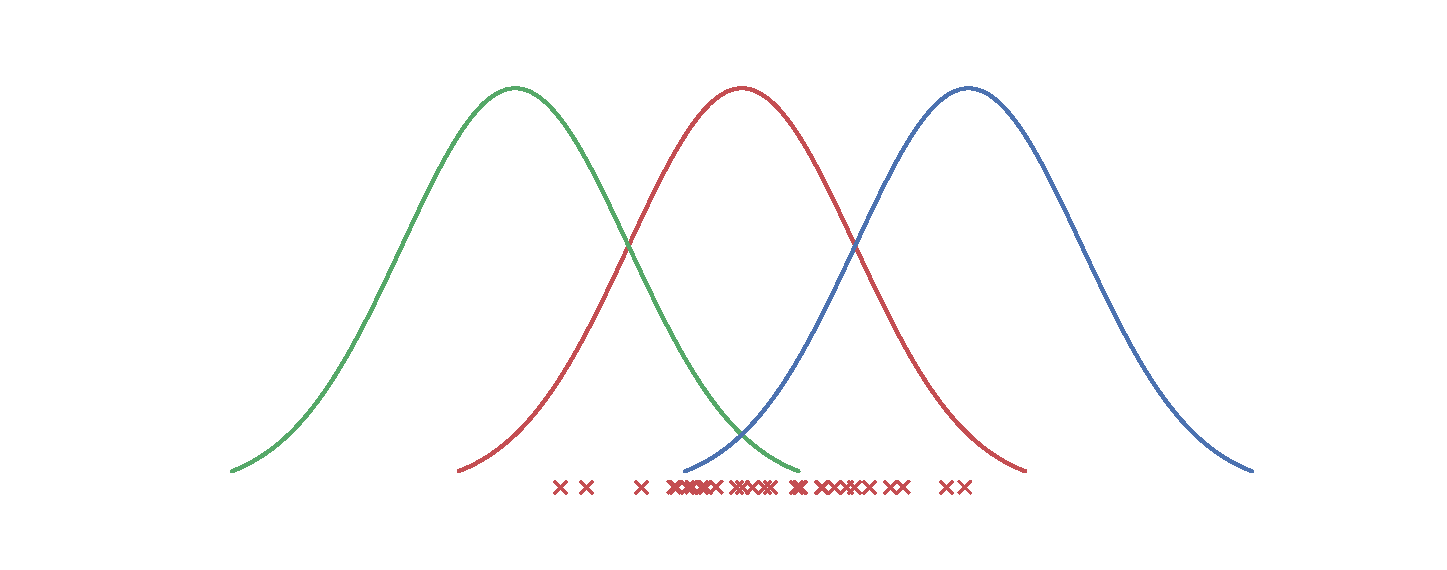
\includegraphics[width=0.5\textwidth]{./figures/MLE.pdf}
  \centering
  \caption{MLE估计高斯分布参数}
  \label{MLE}
\end{figure}

假设数据点表述为$\mathcal{X}=\{x_1, x_2, \cdots, x_n\}$,且每个数据点之间都满足独立同分布条件,
其概率密度函数为$P(X=x|\theta)$,那么所有数据出现的概率就是
\begin{equation}\label{Likelihood}
  \begin{split}
    P(\mathcal{X}|\theta) = \prod_{i=1}^{n}P(x_i|\theta).
  \end{split}
\end{equation}
可以看到公式中数据$\mathcal{X}$是已知的,所以$P(\mathcal{X}|\theta)$是一个关于$\theta$的函数,通常被称作\textbf{似然函数}。

接下来就要寻找能够更好地解释这组数据的参数$\theta$,即使得函数$P(\mathcal{X}|\theta)$的值最大的$\theta$,
写作
\begin{equation}\label{}
  \hat\theta = \argmax_{\theta} \prod_{i=1}^{n}P(x_i|\theta).
\end{equation}
要最大化一个函数的值,我们首先想到的一定是一阶导数为零。但是观察公式 (\ref{Likelihood}),
对于连乘的函数求导并不是一件容易的事情,于是考虑取对数简化运算。

这里有两点考虑:一方面,对数函数能够保持原函数的增减性,所以取对数前后函数的极值点保持一致;
另一方面,对数函数能够变乘法为加法,大大降低了运算难度,也提高了数值的可识别性,
比如概率累乘会出现数值非常小的情况(像1e-30这样的数值),很容易超出计算机的精度产生溢出错误,
而取对数之后,计算机就很容易识别了(对1e-30取以10为底的对数得到-30)。
于是\textbf{对数似然函数}便产生了,如公式 (\ref{LogLikelihood}),
\begin{equation}\label{LogLikelihood}
  \begin{split}
    \mathcal{L}(\theta|\mathcal{X}) &= \mathrm{log}P(\mathcal{X}|\theta)\\
    &= \mathrm{log}\prod_{i=1}^{n}P(x_i|\theta)\\
    &= \sum_{i=1}^{n}\mathrm{log}P(x_i|\theta).
  \end{split}
\end{equation}
注意这里的对数似然函数写成$\mathcal{L}(\theta|\mathcal{X})$而不是$\mathcal{L}(\theta)$,
是因为待估计量(参数)$\theta$是随着观测数据$\mathcal{X}$的变化而变化的。因此优化目标变为:
\begin{equation}\label{}
  \hat\theta = \argmax_{\theta} \sum_{i=1}^{n}\mathrm{log}P(x_i|\theta).
\end{equation}
接下来便是对多维参数求偏导(若是一维参数则直接求导),然后令一阶导数为零,最后一一解出参数的估计值即可。

这里我们以高斯分布为例,进行参数的极大似然估计。

首先高斯分布的概率密度函数为
\begin{equation}
  p(x)= \frac{1}{\sqrt{2 \pi} \sigma}\mathrm{exp}\left(-\frac{(x-\mu)^2}{2\sigma^2}\right),
\end{equation}
假设数据为$X = (x_1,x_2, \cdots,x_n)^T, \quad x_i  \overset{\text{iid}}{\sim} \mathcal{N}(\mu,\sigma^2)$,
可以得到对数似然函数
\begin{equation}
  \begin{split}
    \mathcal{L}(\mu,\sigma|X) &= \sum_{i=1}^{n}\mathrm{log}P(x_i|\mu, \sigma)\\
    &= \sum_{i=1}^{n}{\mathrm{log}\frac{1}{\sqrt{2 \pi} \sigma}\mathrm{exp}\left(-\frac{(x-\mu)^2}{2\sigma^2}\right)}\\
    &= \sum_{i=1}^{n}{\mathrm{log}\frac{1}{\sqrt{2\pi}}+\mathrm{log}\frac{1}{\sigma}-\frac{(x_i-\mu)^2}{2\sigma^2}}.
  \end{split}
\end{equation}
然后用$\mathcal{L}(\mu,\sigma|X)$分别对参数$\mu$和$\sigma$求偏导并令其为零,因为比较容易,
所以这里省略化简过程,最后可以得到参数的估计值:
\begin{equation}
  \begin{split}
    &\hat\mu_{MLE} = \frac{1}{n}\sum_{i=1}^{n}x_i\\
    &\hat\sigma_{MLE}^2= \frac{1}{n}\sum_{i=1}^{n}(x_i-\mu_{MLE})^2.
  \end{split}
\end{equation}
不难发现,用极大似然估计的高斯分布$\hat\mu$为所有样本数据点的均值,$\hat\sigma^2$为所有样本数据点方差。

最后,简单总结一下极大似然估计参数的过程:
\begin{itemize}
  \item[i.] 根据概率密度函数写出似然函数
  \item[ii.] 对似然函数取对数,整理表达式
  \item[iii.] 对表达式求一阶导,令导数为零,得到似然方程
  \item[iv.] 解似然方程,得到参数的估计值
\end{itemize}

\subsection{隐变量}
\label{subsection-2}

在EM算法的学习过程中,经常会看到一个词:\textbf{隐变量}(latent variable),
它是相对于\textbf{观测变量}(obeservable variable)而言的,观测变量一般就指的是数据本身,
那么隐变量到底是什么呢?其实就是未观测到的但是影响观测数据的变量。

下面我们举例进行解释。刚刚在极大似然估计的过程中存在一个假设:所有的数据点来自于同一个分布。
当然这个假设在直观上也是符合认知的,因为图\ref{MLE} 中的那组数据看起来确实像是从同一个高斯分布中抽取出来的。

但是并不是所有问题都符合这种假设,更多的是图\ref{latent variable-1} 中的数据分布,如果我们依旧用单个高斯分布去拟合,
根据章节\ref{subsection-1} 中讨论过的极大似然估计的结果,$\hat\mu$($\mu$的估计值)为样本均值,
$\hat\sigma^2$($\sigma^2$的估计值)为样本方差,因此就会出现图\ref{latent variable-1} 中的情况。
显然,这不是我们想要的。

\begin{figure}[!h]
  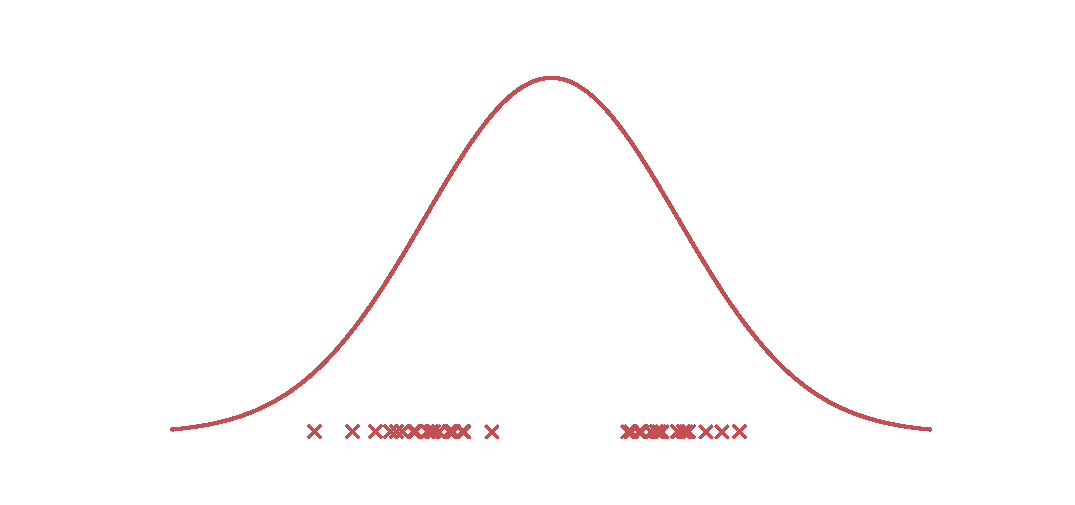
\includegraphics[width=0.5\textwidth]{./figures/LV-1.pdf}
  \centering
  \caption{单高斯拟合含有隐变量的数据}
  \label{latent variable-1}
\end{figure}

很容易想到:我们可以用两个高斯去拟合。这其实就是混合高斯模型的雏形,
其模型思想很简单,如图\ref{latent variable-2} 所示,
当给出的样本是绿色的点时,就用绿色的高斯分布去拟合,
当给出的样本是红色的点时,就用红色的高斯分布去拟合。

\begin{figure}[!h]
  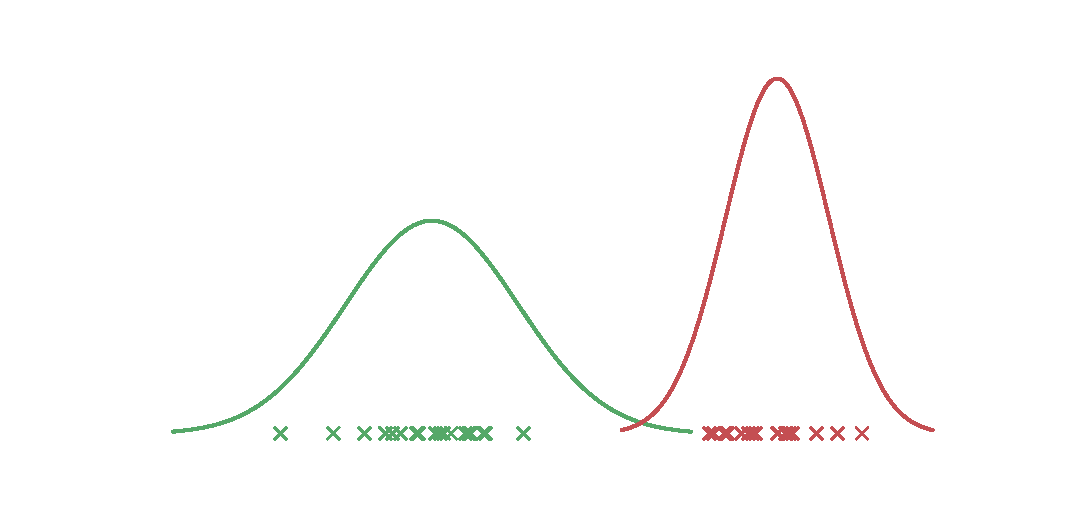
\includegraphics[width=0.5\textwidth]{./figures/LV-2.pdf}
  \centering
  \caption{混合高斯拟合含有隐变量的数据}
  \label{latent variable-2}
\end{figure}

于是,在这个模型中,每一个样本点的解释就分为两步:
第一,这个样本来自于哪个高斯分布,第二,这个高斯分布的参数是什么。
此时\textbf{隐变量}就出现了,它存在于第一步中,用于决定样本来自于哪个高斯分布。
为了让模型更具一般性,假设有$K$个高斯分布,用$z_k={1, 2, \cdots, K}$来表示样本来自于哪个高斯分布,
参数$\theta=\{\mu_1, \cdots, \mu_K; \sigma_1, \cdots, \sigma_K\}$表示每个高斯分布的参数,
那么模型就可以写作:
\begin{equation}
  \begin{split}
    p(x|\theta) &= \sum_{i=1}^{K}p(z_k) \mathcal{N}(\mu_k, \sigma_k)\\
    & \quad\quad \mathrm{s.t.} \quad \sum_{i=1}^{K}p(z_k) = 1,
  \end{split}
\end{equation}
即任意一个样本产生的概率既与决定该样本属于哪个分布的隐变量(此处为$z_k$)有关,
也与产生该样本的分布(此处$\mathcal{N}(\mu_k, \sigma_k)$)有关。

如果将观测数据表示为$X=(x_1, x_2, \cdots, x_n)$,则观测数据的对数似然函数为:
\begin{equation}\label{LogSum}
  \begin{split}
    \mathcal{L}(\theta|X) &= \sum_{i=1}^{n}\mathrm{log}p(x|\theta)\\
    &= \sum_{i=1}^{n}\mathrm{log}\sum_{k=1}^{K}p(z_k) \mathcal{N}(\mu_k, \sigma_k).
  \end{split}
\end{equation}
考虑求模型参数$\theta$的极大似然估计,即
\begin{equation}\label{MaxLLH}
  \hat\theta = \argmax_{\theta}\mathcal{L}(\theta|X).
\end{equation}
按照极大似然估计的步骤,我们应该给$\mathcal{L}(\theta|X)$求偏导并令其为零,然后求解方程得到参数的估计值。

但是从公式(\ref{LogSum}) 可以看到,由于\textbf{隐变量}的引入,
$\mathcal{L}(\theta|X)$的表达实里存在求和之后取对数的情况,
这时想要求导并得到解析解几乎不可能,因此只有通过迭代的方法求解,
而EM算法就是可以用于求解这个问题的一种迭代算法。

\subsection{EM算法}

对于一个迭代算法而言,必须有一个迭代变量,同时也要建立起一个迭代关系,如公式(\ref{IterativeFunction}),
从而让计算机发挥运算速度快、适合做重复运算的优势来进行求解。
\begin{equation}\label{IterativeFunction}
  \theta^{(g+1)} = f \left (\theta^{(g)} \right).
\end{equation}

既然EM算法是一种迭代算法,那么它的迭代变量和迭代关系分别是什么呢?
通常会看到教科书或者网课上给出如公式(\ref{IF4EM}) 所示的迭代关系,
其中,$X$代表所有数据样本,$Z$ 代表隐变量,$\theta$是模型参数,其右上角的角标代表迭代轮数。
\begin{equation}\label{IF4EM}
  \textcolor[rgb]{0.0,0.0,0.8}{\theta^{(g+1)} = \argmax_{\theta} \int_{Z}\mathrm{log}P (X, Z | \theta) P \left(Z|X, \theta^{(g)} \right)dZ}.
\end{equation}
但是为什么是这样的迭代关系呢?我们一步步来分析。

首先,假设迭代关系是对数似然函数,既然我们想要最大化它的值,那么就需要保证每一步迭代的结果都比上一次更好,
即证明
\begin{equation}
  \mathcal{L} \left(\theta^{(g+1)}|X \right) \ge \mathcal{L} \left(\theta^{(g)}|X \right),
\end{equation}
也可以将其展开,
\begin{equation}\label{EMCondition}
  \textcolor[rgb]{0.0,0.0,0.8}{\mathrm{log}P \left(X|\theta^{(g+1)} \right) \ge \mathrm{log} P \left(X|\theta^{(g)}\right)}.
\end{equation}

可以看到,目前为止隐变量还没有出现,下面来看对数似然函数本身,我们结合贝叶斯公式引入隐变量$Z$,
试图简化计算,
\begin{equation}\label{BeforeE}
  \begin{split}
    \mathrm{log}P(X|\theta) &= \mathrm{log} \left\{ \frac{P(X,Z|\theta)}{P(Z|X, \theta)}\right\}\\
    &= \mathrm{log}P(X,Z|\theta) - \mathrm{log}P(Z|X,\theta),
  \end{split}
\end{equation}
然后对其两边依照概率$P(Z|X,\theta^{(g)})$求期望,
\begin{equation}
  \mathbb{E}_{P(Z|X,\theta^{(g)})}\left[\mathrm{log}P(X|\theta)\right] = \mathbb{E}_{P(Z|X,\theta^{(g)})}\left[\mathrm{log}P(X,Z|\theta)\right] - \mathbb{E}_{P(Z|X,\theta^{(g)})}\left[\mathrm{log}P(Z|X,\theta)\right],
\end{equation}
将其写为积分的形式,由于$\mathrm{log}P(X|\theta)$中不含积分变量$Z$,所以先将其提到积分运算之外,
\begin{equation}\label{IntegerSimplify}
  \begin{split}
    \int_{Z}\mathrm{log}P(X|\theta)P\left(Z|X,\theta^{(g)}\right)dZ &= \int_{Z}\mathrm{log}P(X,Z|\theta)P\left(Z|X,\theta^{(g)}\right)dZ - \int_{Z}\mathrm{log}P(Z|X,\theta)P\left(Z|X,\theta^{(g)}\right)dZ\\
    \mathrm{log}P(X|\theta)\int_{Z}P\left(Z|X,\theta^{(g)}\right)dZ &= \int_{Z}\mathrm{log}P(X,Z|\theta)P\left(Z|X,\theta^{(g)}\right)dZ - \int_{Z}\mathrm{log}P(Z|X,\theta)P\left(Z|X,\theta^{(g)}\right)dZ,
  \end{split}
\end{equation}
因为变量空间中所有事件的概率和为1,即$\int_{Z}P(Z|X,\theta^{(g)})dZ = 1$,因此可以将上式化简为
\begin{equation}\label{QH}
  \textcolor[rgb]{0.0,0.0,0.8}{\mathrm{log}P(X|\theta) = \underbrace{\int_{Z}\mathrm{log}P(X,Z|\theta)P\left(Z|X,\theta^{(g)}\right)dZ}_{Q\left(\theta,\theta^{(g)}\right)} - \underbrace{\int_{Z}\mathrm{log}P(Z|X,\theta)P\left(Z|X,\theta^{(g)}\right)dZ}_{H\left(\theta, \theta^{(g)}\right)}}.
\end{equation}

至此,我们有一个问题还没有考虑:为什么要依照概率$P(Z|X,\theta^{(g)})$求期望呢?
$P(Z|X,\theta^{(g)})$代表了给定观测数据$X$和第$g$轮参数估计$\theta^{(g)}$下隐变量数据$Z$的
条件概率分布,由于$Z$是未观测数据,是用于简化计算的辅助变量,所以必须保证它不能影响结果,
也就是说在求第$g+1$轮的参数估计$\theta^{(g+1)}$时,必须保证在给定数据$X$的情况下,
$\theta$是唯一影响对数似然函数取值的因素,这就要求剔除$Z$的影响,
因而对公式(\ref{BeforeE}) 依照概率$P(Z|X,\theta^{(g)})$求期望从而将$Z$消掉。

回到证明EM算法的收敛性上来,即证明公式(\ref{EMCondition}) 成立,结合公式(\ref{QH}) 可将问题转化为
证明下式成立:
\begin{equation}\label{EMFinalCondtion}
  Q \left(\theta^{(g+1)},\theta^{(g)}\right) - H\left(\theta^{(g+1)}, \theta^{(g)}\right) \ge Q\left(\theta^{(g)},\theta^{(g)}\right) - H\left(\theta^{(g)},\theta^{(g)}\right).
\end{equation}

不难发现,公式(\ref{QH}) 中的$Q\left(\theta,\theta^{(g)}\right)$其实就是EM算法迭代函数中最大化的对象,
结合它将公式(\ref{IF4EM}) 改写一下可以得到:
\begin{equation}\label{QFunction}
  \forall \theta, Q \left(\theta^{(g+1)},\theta^{(g)}\right) \ge Q\left(\theta,\theta^{(g)}\right).
\end{equation}
也就是说,左边式子是个值,右边式子是个函数,而且不论右边式子中的变量$\theta$取任何值,都不会大于左边式子的值,
因而左边式子的值是右边函数的最大值,所以当$\theta = \theta^{(g)}$时,上式依然成立,即
\begin{equation}\label{Qresult}
  Q \left(\theta^{(g+1)},\theta^{(g)}\right) \ge Q\left(\theta^{(g)},\theta^{(g)}\right).
\end{equation}

接下来证明$H$项,既然$Q$项已经满足公式(\ref{Qresult}) 了,那么如果$H$项能满足
\begin{equation}\label{Hresult}
  H \left(\theta^{(g+1)},\theta^{(g)}\right) \le H\left(\theta^{(g)},\theta^{(g)}\right).
\end{equation}
我们就可以完成公式(\ref{EMFinalCondtion})证明了。
要证明上式成立,我们也可以构造类似公式(\ref{QFunction}) 的不等式,即
\begin{equation}\label{HFunction}
  \forall \theta, H\left(\theta,\theta^{(g)}\right) \le H \left(\theta^{(g)},\theta^{(g)}\right).
\end{equation}
如果这个式子成立,那么就可以同样的令$\theta = \theta^{(g+1)}$从而证明公式(\ref{Hresult}) 成立。
要证这个式子成立,需要参考公式(\ref{QH})和Jensen不等式,有
\begin{equation}\label{HProve}
  \begin{split}
    & H \left(\theta,\theta^{(g)}\right) - H \left(\theta^{(g)},\theta^{(g)}\right)\\
    =& \int_{Z}\mathrm{log}P(Z|X,\theta)P\left(Z|X,\theta^{(g)}\right)dZ - \int_{Z}\mathrm{log}P(Z|X,\theta^{(g)})P\left(Z|X,\theta^{(g)}\right)dZ\\
    =& \int_{Z}\mathrm{log}\frac{P(Z|X,\theta)}{P\left(Z|X,\theta^{(g)}\right)}P\left(Z|X,\theta^{(g)}\right)dZ\\
    \le& \mathrm{log}\int_{Z}\frac{P(Z|X,\theta)}{P\left(Z|X,\theta^{(g)}\right)}P\left(Z|X,\theta^{(g)}\right)dZ\\
    =& \mathrm{log}\int_{Z}P(Z|X,\theta)dZ\\
    =& \mathrm{log}1\\
    =& 0
  \end{split}
\end{equation}
因而公式(\ref{HFunction}) 是成立的,所以公式(\ref{EMFinalCondtion}) 得证。
综上所述,EM算法是会随着迭代的进行一步步收敛到极值的。

在公式(\ref{HProve}) 的证明中,出现不等式的那一步利用了所谓的Jensen不等式,
简单来讲,Jensen不等式描述了:在凸函数中(这里指下凸函数),
函数的期望不小于期望的函数,或者说
在凹函数中,函数的期望不大于期望的函数。

其实它很容易理解,如图\ref{FigJensen} 所示,
可以看到,对于点$x1$和$x2$,
函数的期望为$p1*f(x1)+p2*f(x2)$,期望的函数为$f(p1*x1+p2*x2)$,
显然,假设约束$p1+p2=1, p1>0, p2>0$一直满足,那么无论$p1$和$p2$如何变化,
$p1*f(x1)+p2*f(x2) \le f(p1*x1+p2*x2)$总是成立,即函数的期望总是不大于期望的函数。

\begin{figure}[!h]
  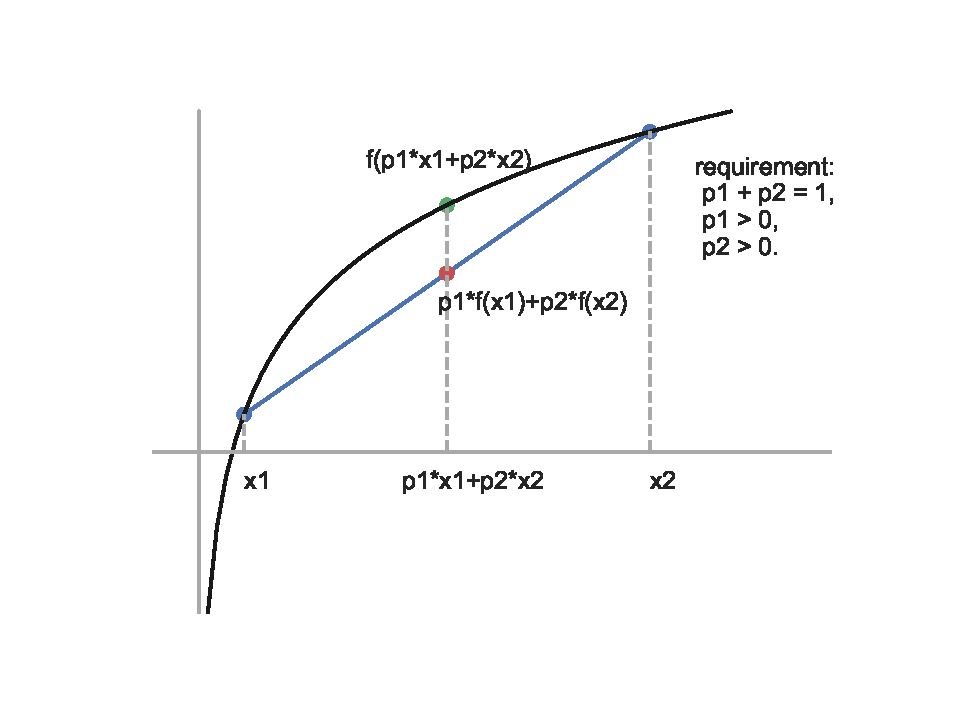
\includegraphics[width=0.5\textwidth]{./figures/Jensen.pdf}
  \centering
  \caption{Jensen不等式图示}
  \label{FigJensen}
\end{figure}

结合公式(\ref{HProve}) 来说,这里的函数指的是$\mathrm{log(x)}$,
而对于连续的变量通常使用积分来替代期望,所以下式很容易成立,
\begin{equation}\label{JensenInHP}
  \int_{Z}\mathrm{log}\frac{P(Z|X,\theta)}{P\left(Z|X,\theta^{(g)}\right)}P\left(Z|X,\theta^{(g)}\right)dZ
  \le \mathrm{log}\int_{Z}\frac{P(Z|X,\theta)}{P\left(Z|X,\theta^{(g)}\right)}P\left(Z|X,\theta^{(g)}\right)dZ.
\end{equation}
这样一来,公式(\ref{HProve}) 中后半部分的证明就顺利成章了。

其实,以上的推导也在一定程度上解答了另外一个问题:为什么不直接优化对数似然函数而是选择优化$Q$函数。因为在迭代时,要保证优化过程的收敛,就必须保证对数似然函数在逐步最大化,而对数似然函数由两部分组成,
\begin{equation}
  \mathcal{L}(\theta|X) = Q \left(\theta, \theta^{(g)} \right) - H \left(\theta, \theta^{(g)} \right),
\end{equation}
其中,可以证明$H$函数是逐步变小的,那么$-H$就是逐步变大的,所以要保证对数似然函数逐步变大,只要保证$Q$函数逐步变大即可,因此,既然可以通过优化形式相对简单的$Q$函数达到目的,那么就不必要在EM算法中优化整个对数似然函数了。

到这里,EM算法的推导与收敛证明就告一段落了,下面给出EM算法的一般流程。

\begin{algorithm}[htb]
  \caption{EM算法}
  \label{alg:em}
  \begin{algorithmic}[1]
    \Require
    观测变量数据$X$,隐变量数据$Z$,联合分布$P(X,Z|\theta)$,条件分布$P(Z|X,\theta)$;
    \Ensure
    模型参数$\theta$。
    \State 选择参数的初始值$\theta^{(0)}$,开始迭代;
    \label{code:em:init}
    \State $\mathrm{E}$步:记$\theta^{(g)}$为第$g$次迭代参数$\theta$的估计值,在第$g+1$次迭代的E步,计算
    \begin{equation}
      \begin{split}
        Q\left(\theta, \theta^{(g)}\right) &= \mathbb{E}_{P(Z|X,\theta^{(g)})}\left[\mathrm{log}P(X,Z|\theta)\right]\\
        &= \int_{Z}\mathrm{log}P (X, Z | \theta) P \left(Z|X, \theta^{(g)} \right)dZ.
      \end{split}
    \end{equation}
    这一步主要目的是计算$P(Z|X,\theta^{(g)})$,它代表了给定观测数据$X$和第$g$轮参数估计$\theta^{(g)}$下
    隐变量数据$Z$的条件概率分布;
    \label{code:em:e}
    \State $\mathrm{M}$步:求使$Q\left(\theta, \theta^{(g)}\right)$极大化的$\theta$,确定第$g+1$轮参数的估计值$\theta^{(g+1)}$
    \begin{equation}
      \theta^{(g+1)} = \argmax_{\theta}Q\left(\theta, \theta^{(g)}\right).
    \end{equation}
    \label{code:em:m}
    \State 重复第\ref{code:em:e} 步和第\ref{code:em:m} 步,直到收敛。
    \label{code:em:loop}
  \end{algorithmic}
\end{algorithm}

算法\ref{alg:em} 中提到了收敛,那么到底什么时候才算收敛呢?通常会这么做,对于较小的正数$\varepsilon_1, \varepsilon_2$,若满足
\begin{equation}
  \left\Vert \theta^{(g+1)}-\theta^{(g)} \right\Vert \le \varepsilon_1 \quad or \quad \left\Vert Q\left(\theta^{(g+1)}, \theta^{(g)}\right) - Q\left(\theta^{(g)}, \theta^{(g)}\right) \right\Vert \le \varepsilon_2,
\end{equation}
则迭代停止。

\subsection{高斯混合模型}

高斯混合模型(Guassian Mixture Model, 简称GMM),为单一高斯概率密度函数的延伸,用多个高斯概率密度函数(正态分布曲线)精确地量化变量分布,是将变量分布分解为若干基于高斯概率密度函数(正态分布曲线)分布的统计模型。

图\ref{SGM-model&GMM-model}分别用单高斯模型和混合高斯模型分析同一组样本点。图\ref{SGM-model} 使用单个二维高斯分布来描述数据,椭圆即为二倍标准差的正态分布椭圆。图\ref{GMM-model} 使用两个二维高斯分布来描述数据,分别记为$\mathcal N({\mu}_1,{\Sigma}_1)$和$\mathcal N({\mu}_2,{\Sigma}_2)$,两个椭圆分别是这两个高斯分布的二倍标准差椭圆。

\begin{figure}[!h]
	\centering
	\subfigure[]{
		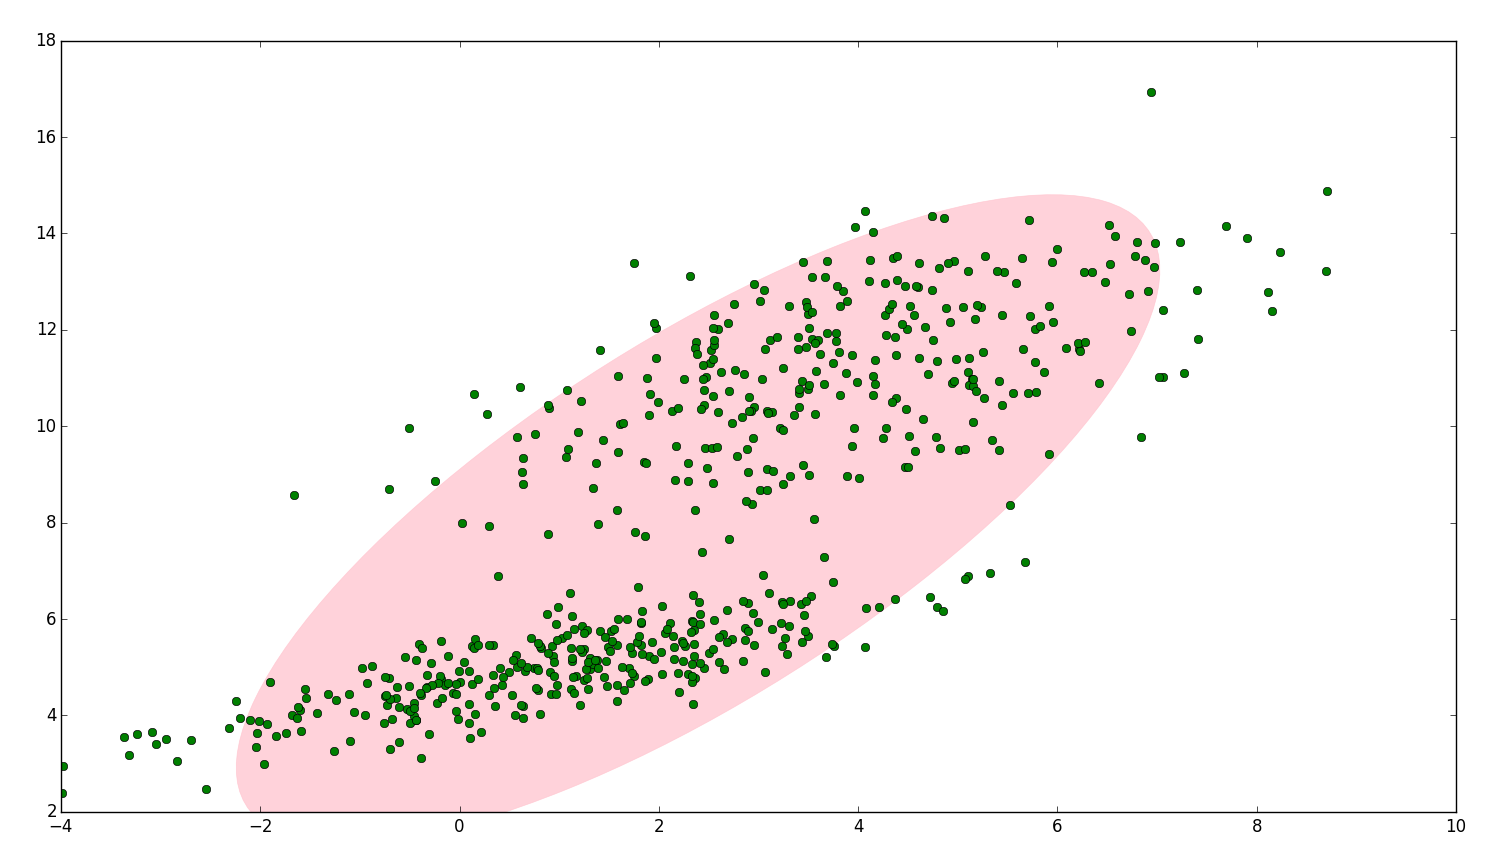
\includegraphics[width=0.45\textwidth]{figures/SGM.jpg}
		\label{SGM-model}
	}\quad  
	\subfigure[]{
		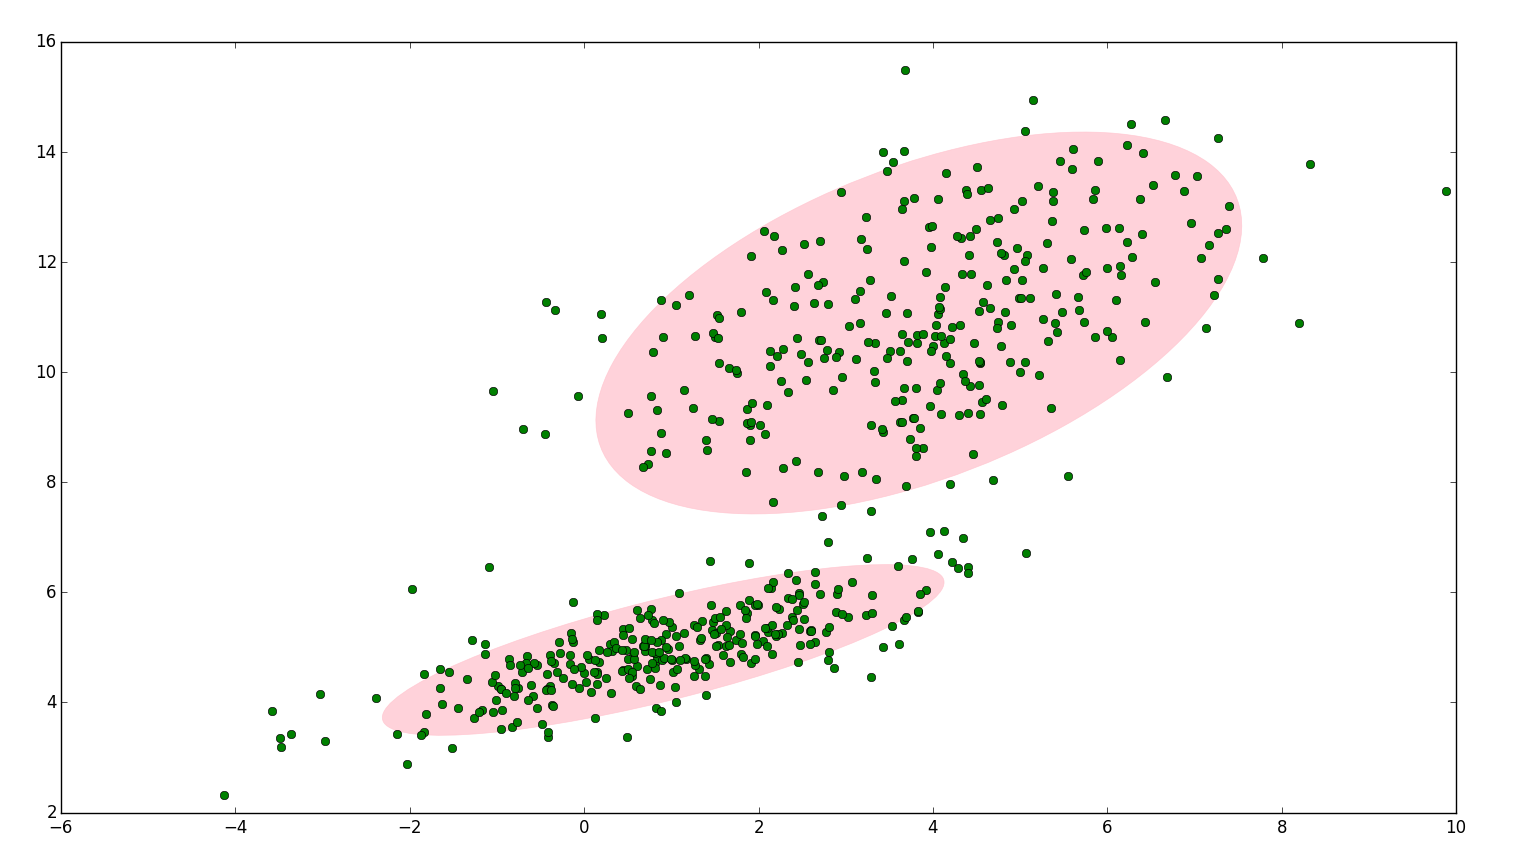
\includegraphics[width=0.45\textwidth]{figures/GMM.jpg}
		\label{GMM-model}
	}
	\caption{单个二维高斯分布拟合数据 \& 两个二维高斯分布拟合数据}
	\label{SGM-model&GMM-model}
\end{figure}

可以看到使用两个二维高斯分布来描述图中的数据显然更合理。实际上图中的两个聚类的中的点是通过两个不同的正态分布随机生成而来。如果将两个二维高斯分布为$\mathcal N({\mu}_1,{\Sigma}_1)$和$\mathcal N({\mu}_2,{\Sigma}_2)$合成一个二维的分布,那么就可以用合成后的分布来描述图\ref{GMM-model}中的所有点。最直观的方法就是对这两个二维高斯分布做线性组合,用线性组合后的分布来描述整个集合中的数据。

提出混合模型主要是为了能更好地近似一些较复杂的样本分布,通过不断增加单个分布的个数,可以任意地逼近任何连续的概率分布,所以我们认为任何样本分布都可以用混合模型来建模。为什么我们要假设数据是由若干个高斯分布组合而成的,而不假设是其他分布呢?实际上不管是什么分布,只要数量取得足够大,这个混合模型就会变得足够复杂,就可以用来逼近任意连续的概率密度分布。只是因为高斯函数具有良好的计算性能,所以GMM被广泛地应用。

GMM与Kmeans类似,也是常见的聚类算法。不同的是,Kmeans把每个样本点分配到其中某一个cluster,而GMM是学习出一些概率密度函数,给出这些样本点分配到每个cluster的概率,每个单分布就是一个聚类中心,也称为软聚类。所以GMM不仅仅可以用于聚类,还可以用于概率密度的估计。

设有随机变量$X$,则GMM的概率密度函数可以用式(\ref{GMM})表示:
\begin{equation}\label{GMM}
  \begin{split}
    p(x) &= \sum_{k=1}^{K}p(k)p(x|k)\\
    &= \sum_{k=1}^{K}\pi_k\mathcal{N}\left(x\big|\mu_k, \Sigma_k\right).
  \end{split}
\end{equation}

其中$\mathcal{N}(x|\mu_k, \Sigma_k)$称为混合模型中的第$k$个组件(component)。$\pi_k$是混合系数(mixture coefficient),且满足$\sum_{k=1}^K\pi_k = 1(0\le\pi_k\le1)$。实际上,可以认为$\pi_k$就是每个分量$\mathcal{N}(x|\mu_k, \Sigma_k)$的权重。

根据式(\ref{GMM}) ,如果我们要从GMM分布中随机地取一个点,需要两步:第一,随机地在这$K$个组件之中选一个,每个组件被选中的概率实际上就是它的系数$\pi_k$;第二,选中了组件之后,再单独地考虑从这个组件的分布中选取一个点。

对一个样本集建立高斯混合模型的过程,就是根据已知样本集X反推高斯混合模型的参数$(\mu,\sigma,\pi)$,这是一个参数估计问题。首先想到用最大似然的方法求解,也就是,要确定参数$\mu,\sigma,\pi$使得它所确定的概率分布生成这些样本点的概率最大,这个概率也就是似然函数,如下:
\begin{equation}
  p(x) = \prod_{i=1}^{N}x_k.
\end{equation}
而一般对于单个样本点其概率较小,多个相乘后更小,容易造成浮点数下溢,所以一般是对似然函数求对数,变成加和形式:$\sum_{i=1}^{N}\ln p(x_i)$。这个叫做log似然函数,目标是要最大化它。用log似然函数对参数分别求偏导,令偏导等于0,可求解得参数。然而,GMM的log似然函数是如下形式:
\begin{equation}
  \ln L(\mu,\sigma,\pi) = \sum_{i=1}^{N}\ln\sum_{k=1}^{K}\pi_k\mathcal{N}\left(y_n\big|\mu_k,\sigma_k\right).
\end{equation}

可以看到对数中有求和,直接求导求解将导致一系列复杂的运算,无法求出这个对数似然函数的最大值,故考虑使用EM算法。

那么极大似然估计与EM算法分别适用于什么问题呢?如果我们已经清楚某个变量服从高斯分布,而且通过采样得到了这个变量的样本数据,想要求高斯分布的参数,这时候极大似然估计可以胜任这个任务;而如果我们要求解的是一个混合模型,只知道混合模型中各个类的分布模型(譬如都是高斯分布)和对应的采样数据,而不知道这些采样数据分别来源于哪一类(隐变量),那这时候就可以借鉴EM算法。EM算法可以用于解决数据缺失的参数估计问题(隐变量的存在实际上就是数据缺失问题,缺失了各个样本来源于哪一类的记录)。

EM算法分两步,第一步先求出要估计参数的粗略值,第二步使用第一步的值最大化似然函数。因此要先求出GMM的似然函数。

考虑GMM生成一个样本点的过程,这里对每个$\mathbf x_i$引入隐变量$\mathbf z$,$\mathbf z$是一个$K$维向量,如果生成$\mathbf x_i$时选择了第$k$个component,则$\mathbf z_k=1$,其他元素都为0,$\sum_{k=1}^{K}z_k=1$.

假设$\mathbf z$是已知的,则样本集变成了${X,Z}$,要求解的似然函数变成了:
\begin{equation}
  p\left(X,Z\big|\mu,\sum,\pi\right) = \prod_{n=1}^N\prod_{k=1}^K\pi_k^{z_{nk}}\mathcal N\left(\mathbf x_n\big|\mu_k,\sum_k\right)^{z_{nk}}.
\end{equation}
log似然函数为:
\begin{equation}\label{loglikelihood}
  \ln p\left(X,Z\big|\mu,\sum,\pi\right) = \sum_{n=1}^N\sum_{k=1}^K\mathbf z_{nk}\left[\ln\pi_k + \ln\mathcal N\left(\mathbf x_n\big|\mu_k,\sum_k\right)\right].
\end{equation}

可以看到,这次 ln 直接对Gaussian作用,求和在 ln 外面,所以可以直接求最大似然解了。

\textbf{EM算法估计GMM参数的过程如下:}

\textbf{1. 初始化一组参数$\mu ^0,\Sigma ^0,\pi ^0$}

\textbf{2. E-step}

然而,事实上$\mathbf z$是不知道的,我们只是假设$\mathbf z$已知。而$\mathbf z$的值是通过后验概率观测,所以这里考虑用$\mathbf z$值的期望在上述似然函数中代替$\mathbf z$。

对于一个样本点$\mathbf x$:
\begin{equation}
  p(\mathbf z) = \prod_{k=1}^K\pi_k^{z_k}.
\end{equation}
\begin{equation}
  p(\mathbf x|\mathbf z_k=1) = \mathcal N\left(\mathbf x\big|\mu_k,\sum_k\right).
\end{equation}
\begin{equation}
  p(\mathbf x|\mathbf z) = \prod_{k=1}^K\mathcal N\left(\mathbf x\big|\mu_k,\sum_k\right)^{z_k}.
\end{equation}
\begin{equation}
  \begin{split}
    p(\mathbf x) &= \sum_zp(\mathbf z)p(\mathbf x|\mathbf z)\\
    &= \sum_{k=1}^K\pi_k\mathcal N\left(\mathbf x\big|\mu_k,\sum_k\right).
  \end{split}
\end{equation}

后验概率(固定$\mu,\sum,\pi$):
\begin{equation}
  p\left(\mathbf z\big|\mathbf x,\mu,\sum,\pi\right) = \frac{p(\mathbf x|\mathbf z)p(\mathbf z)}{p(\mathbf x)} \propto \prod_{n=1}^N\prod_{k=1}^K\left[{\pi_k\mathcal N\left(x_n\big|\mu_k,\sum_k\right)}\right]^{z_{nk}}.
\end{equation}

因为${\mathbf z_n}$之间是相互独立的。

计算$\mathbf z$期望$\gamma(\mathbf z_{nk})$(z向量只有一个值取1,其余为0):
\begin{equation}
  \begin{split}
    \gamma(\mathbf z_{nk}) &= E[\mathbf z_{nk}]\\
    &= 0*p(\mathbf z_{nk}=0|\mathbf x_n)+1*p(\mathbf z_{nk}=1|\mathbf x_n)\\
    &=p(\mathbf z_{nk}=1|\mathbf x_n)\\
    &=\frac{p(\mathbf z_{nk}=1)p(\mathbf x_n|\mathbf z_{nk}=1)}{p(\mathbf x_n)}\\
    &=\frac{\pi_k\mathcal N\left(\mathbf x\big|\mu_k,\sum_k\right)}{\sum_{j=1}^K\pi_j\mathcal N\left(\mathbf x\big|\mu_j,\sum_j\right)}.
  \end{split}
\end{equation}

将$\mathbf z$值用期望代替,则待求解的log似然函数(\ref{loglikelihood})式变为:
\begin{equation}
  E_z\left[\ln p\left(X,Z\big|\mu,\sum,\pi\right)\right] = \sum_{n=1}^N\sum_{k=1}^K\gamma (\mathbf z_{nk})\left[\ln\pi_k + \ln\mathcal N\left(\mathbf x_n\big|\mu_k,\sum_k\right)\right].
\end{equation}

\textbf{3. M-step}

现在可以最大化似然函数求解参数了,首先对$\mu$求偏导,令偏导等于0,可得:
\begin{equation}
  \sum_{n=1}^N\sum_{k=1}^K\gamma (\mathbf z_{nk})\sum_k(\mathbf x_n-\mu_k) = 0.
\end{equation}
\begin{equation}
  \mu_k = \frac{1}{N_k}\sum_{n=1}^N\gamma (\mathbf z_{nk}){\mathbf x_n},\text{其中}N_k = \sum_{n=1}^N\gamma (\mathbf z_{nk}).
\end{equation}

再对$\sum_k$求偏导,令偏导等于0,可得:
\begin{equation}
  \sum_k = \frac{1}{N_k}\sum_{n=1}^N\gamma (\mathbf z_{nk})(\mathbf x_n-\mu_k)(\mathbf x_n-\mu_k)^T.
\end{equation}

接下来还需求解$\pi$,注意到$\pi$需满足$\sum_{k=1}^K\pi_k=1$,所以这是一个带等式约束的最大值问题,使用拉格朗日乘数法。

构造拉格朗日函数:
\begin{equation}
  L=\ln p\left(X\big|\pi,\mu,\sum\right)+\lambda\left(\sum_{k=1}^K\pi_k-1\right).
\end{equation}

对$\pi$求导,令导数为0:
\begin{equation}
  \sum_{n=1}^N\frac{\mathcal N\left(\mathbf x\big|\mu_k,\sum_k\right)}{\sum_{j=1}^K\pi_j\mathcal N\left(\mathbf x\big|\mu_j,\sum_j\right)}+\lambda=0.
\end{equation}

两边同乘$\pi_k$得:
\begin{equation}
  \sum_{n=1}^N\gamma (\mathbf z_{nk}) + \lambda\pi_k=0.
\end{equation}
\begin{equation}
  N_k+\lambda\pi_k=0.
\end{equation}

两边对k求和:
\begin{equation}
  \sum_{k=1}^KN_k+\sum_{k=1}^K\lambda\pi_k=0.
\end{equation}
\begin{equation}
  N+\lambda=0.
\end{equation}

可得:$\lambda=-N$

代入可得:$\pi_k=\frac{N_k}{N}.$

\textbf{4. 检查是否收敛}

重复E-step和M-step两步,直到收敛,即可求得一个局部最优解。


\section{应用问题描述}

本次我们采用GMM模型解决两大问题,图像聚类和图像生成,具体任务我们采用MNIST数据集进行验证。对于图像聚类问题,我们采用整体聚类和单类别标签建模的方法分别进行标签预测,而图像生成我们则是先用自编码器进行降维,然后用GMM模型进行数据拟合和新样本生成。


\section{实验}

\subsection{数据集与评价指标}

\subsubsection{数据集}
本实验采用的MNIST数据库是由Yann LeCun教授提供的手写数字数据库文件,该数据集包含了60000张训练图像和10000张测试图像。这些数字已经过尺寸标准化并位于图像中心,且图像是$28 \times 28$大小的灰度图像,每个像素是一个八位字节。数据集共包括四个文件,一个训练图片集train-images-idx3-ubyte.gz,一个训练标签集train-labels-idx1-ubyte.gz,一个测试图片集t10k-images-idx3-ubyte.gz,一个测试标签集t10k-labels-idx1-ubyte.gz。上述四个文件直接解压就可以使用了。

\subsubsection{评价指标}

在本实验中,手写数字识别的评价指标采用了调整兰德系数(Adjusted rand index),正确率(accuracy),查准率(precision),查全率(recall),F1分数(F1-Score)。

兰德系数(Rand index)需要给定实际类别信息 $C$,假设$K$是聚类结果,$a$表示在$C$与$K$中都是同类别的元素对数,$b$表示在$C$与$K$中都是不同类别的元素对数,则兰德系数为:
\begin{equation}
\mathrm{RI}=\frac{a+b}{C_{2}^{n_{samples}}}.
\end{equation}

其中$C_{2}^{n_{samples}}$为数据集中可以组成的总元素对数,RI取值范围为$[0,1]$,值越大意味着聚类结果与真实情况越吻合。调整兰德系数(Adjusted rand index)具有更高的区分度:
\begin{equation}
\mathrm{ARI}=\frac{\mathrm{RI}-E[\mathrm{RI}]}{\max (\mathrm{RI})-E[\mathrm{RI}]}.
\end{equation}

ARI取值范围为$[-1,1]$,值越大意味着聚类结果与真实情况越吻合。从广义的角度来讲,ARI衡量的是两个数据分布的吻合程度。

对于二分类问题,可将样例根据其真实类别和分类器预测类别划分为:
\begin{itemize}
	\item TP:真实类别为正例,预测类别为正例。
	\item FP:真实类别为负例,预测类别为正例。
	\item FN:真实类别为正例,预测类别为负例。
	\item TN:真实类别为负例,预测类别为负例。
\end{itemize}

正确率是我们最常见的评价指标,表示被分对的样本数在所有的样本数中所占比例,即:
\begin{equation}
accuracy = \frac{TP+TF}{TP+FP+FN+TN}.
\end{equation}
通常来说,正确率越高,分类器越好。

查准率是精确性的度量,表示被分为正例的示例中实际为正例的比例,即:
\begin{equation}
	precision = \frac{TP}{TP+FP}.
\end{equation}

查全率也叫做敏感度,表示正例被分类器正确探测出的比率,即:
\begin{equation}
	recall = \frac{TP}{TP+FN}.
\end{equation}

F1分数是统计学中用来衡量二分类模型精确度的一种指标,它同时兼顾了分类模型的查准率和查全率。F1分数可以看作是模型查准率和查全率的一种加权平均,它的最大值是1,最小值是0。数学定义如下:
\begin{equation}
	F1 = \frac{2\times{precision}\times{recall}}{precision+recall}.
\end{equation}

对于多分类问题,我们可以看作是n个二分类问题。正确率的计算方式显然与二分类相同,对于其他的评价指标,分为宏平均(Macro-averaging)和微平均(Micro-averaging)两种情况来进行综合考察。

宏平均先分别计算各类的precision和recall,得到各类的F1,然后再计算F1的平均值。由此可以得到宏查准率(macro-P)、宏查全率(macro-R)、宏F1(macro-F1):
\begin{equation}
	marcoP=\frac{1}{n}\sum_1^nP_i.
\end{equation}
\begin{equation}
	marcoR=\frac{1}{n}\sum_1^nR_i.
\end{equation}
\begin{equation}
	marcoF1=\frac{1}{n}\sum_1^nF1_i.
\end{equation}

微平均将n个二分类评价的TP、FP、FN对应相加,计算出所有类别总的Precision和Recall,再计算得到F1。经过推导可知,此时满足:
\begin{equation}
	microP=microR=microF1=accuracy
\end{equation}

\subsection{实验设置}

本次实验主要分为三部分,第一部分为采取GMM模型对MNIST数据集进行聚类,然后通过$Adjusted~rand~index$,$accuracy$,$precision$,$recall$,$F1$这些评价标准对聚类的结果进行一个评判;第二部分则是包含采用GMM模型直接对MNIST数据集中的每一类样本进行单独建模,最后采用最大似然的方法对新来的测试样本进行预测,从而解决了MNIST数据集上的分类任务;最后一部分则是在MNIST数据集上实现新的样本生成。

\subsubsection{整体聚类}

聚类任务主要分为三个步骤,数据预处理,模型学习,性能评估。

(1)\textbf{数据预处理}

MNIST数据集原始是6万张训练样本,1万张测试样本。由于本部分主要是用于检验聚类任务,因此训练集和测试集的划分的必要性不是很大,因此,我们将训练集和测试集融合,形成了7万张样本以及包含其对应标签,我们的目标是为了将这7万张样本通过无监督的聚类方法将其聚成若干类,然后检验聚类结果。

由于每个样本图片可以视为一个$28 \times 28$的矩阵,我们先采用归一化的方法将矩阵的像素值调整在[0,1]之间,然后采用flatten技术将这个$28 \times 28$的矩阵拍平为长度为784维的向量。那么问题来了,对于784维的特征,显然过于冗长,因此需要考虑将其进行压缩,在此我们选取课程学习的经典降维方法主成分分析(Principal Component Analysis,PCA),对这784维长度的向量进行降维,而降维后的维度$d$我们将其视为一个超参数,通过调整不同的$d$得到不同的评测结果,最终可以选取最优评测结果对应的参数$d$作为最终最优的超参数值。PCA降维的原理图如下所示:

\begin{figure}[!h]
  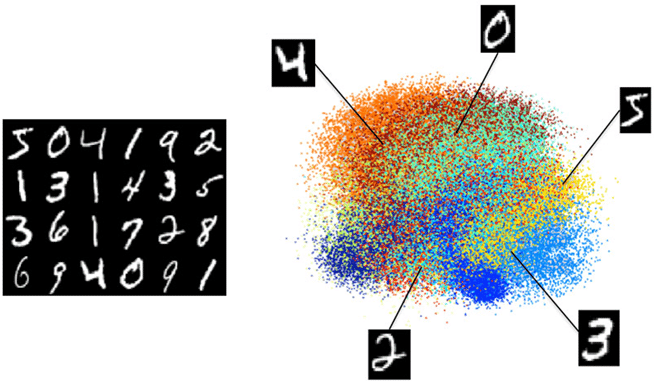
\includegraphics[width=0.5\textwidth]{./figures/PCA_mnist.png}
  \centering
  \caption{PCA原理图}
  \label{PCA-model}
\end{figure}


(2)\textbf{模型学习}

实际上,由于MNIST数据集我们是已知先验知识为10个类别,因此我们选取含有10个高斯分布的GMM模型对这7万张图片进行聚类。同时在聚类结束后给出这7万张图片预测的标签。

(3)\textbf{性能评估}

关于性能评估,首先是对于聚类结果的一个直观上的评估,即判断聚类的每一类是否与真实的类分布吻合,因此很自然我们采用$Adjusted~rand~index$这个评价标准来评判聚类的效果。调整兰德指数通过考虑所有样本并计算在预测的聚类和真实的聚类中分配在相同或不同聚类中的对来计算两个聚类之间的相似性度量。

此外除了衡量聚类的结果,我们进一步想通过聚类的结果对样本的标签进行预测。因此我们提出了一种新的与标签相关的评测方法:具体来说,对于已经无监督聚类得到这10个未知的类之后,我们对每一类的真实标签进行计数统计,选取票数最高的真实标签作为预测的标签,并作为整个聚类簇的标签,最后我们将这所有样本预测的标签与真实的标签进行对比,便可计算出$accuracy$,$precision$,$recall$,$F1$这些常见的分类评价指标。

\subsubsection{单独聚类}

(1)\textbf{数据预处理}

这里我们采用原始 MNIST 数据集的训练集测试集划分,原始的手写数字维度为$28 \times 28$,我们在聚类中弱化其空间结构,将其展开为784维的向量。众所周知,手写数字中存在很多空白的像素,而他们对于我们的聚类任务来说是不太重要的,因此考虑在聚类前使用PCA进行降维,保留更为重要的维度进行聚类,同时数据维度的降低也可以提升模型学习的速度和精度,使得模型取得更好的表现。

(2)\textbf{模型学习}

由于每一个数字的手写方法可能不唯一,而直接聚类可能存在重复类别的问题,直观的讲,假如数字4有5种不同的写法,如果用直接聚类去做的话,我们很难保证最后的聚类结果中不会出现两个表征数字4的类,这样就有可能会挤掉其他的类,如此一来,就会使得聚类结果不太理想。于是考虑分类别聚类,顾名思义,就是对于每一个类别,选取相对应的子数据集,然后训练一个高斯混合模型来表征这个类别,这样就可以捕获同一数字不同的写法,达到更好的识别效果。

(3)\textbf{性能评估}

模型学习结束后,我们会得到10个GMM模型,每个模型对应于一个数字的分布,该分布一般具有多峰性,其不同的峰代表该数字不同的写法。当我们拿到一个新数据时,模型会分别计算其在每一个数字类上的似然,然后选取似然最大的数字类作为最后的预测结果,从而评估模型的性能。因为整个模型看起来类似于多分类任务,所以选择$accuracy$,$precision$,$recall$,$F1$作为衡量指标。

\subsubsection{生成手写数字}

(1)\textbf{数据预处理}

原始数据集包含60000张训练图像和10000张测试图像,我们也按照这种方式进行划分。其中,每张图像的大小为$28 \times 28$。GMM可能难以在如此高维空间中收敛,为了便于之后进行GMM无监督学习,降维方法是必要的。这里我们采用自动编码器,并选取SELU为激活函数。由于SELU具有自归一化的特性,压缩空间将收敛为定义明确的均值和方差。代表压缩空间的某些分布可能是高斯分布的,这样就可以通过高斯混合模型很好地捕获。另外,我们将L2正则化用于编码层以约束其权重空间。

(2)\textbf{手写数字生成}

在MNIST数据集从784维($28 \times 28$)的图像压缩到6维空间之后,我们将高斯混合模型拟合到压缩空间,然后就可以在压缩空间中从高斯混合模型采样新图像。接下来对采样的压缩空间用之前训练的SELU解码器及进行解码,就能得到新的手写数字。这样,我们就以GMM作为生成模型得生成了新的手写数字。

\subsection{实验环境}

我们的实验运行在一个单机Linux服务器上,机器内存64G,2颗Intel Xeon E5-2680 v2的CPU以及4颗GeForce GTX 1080 Ti的GPU(未用到),具体硬件配置如~\ref{tab:hard} 所示。

\begin{table}[!h]
  \centering
  \caption{实验环境硬件配置}\label{tab:hard}
  \begin{tabular}{cc}
    \toprule
    项目 & 配置 \\
    \midrule
    CPU & Intel(R) Xeon(R) CPU E5-2650 v2, 2.60GHz\\
    GPU & GeForce GTX 1080 Ti, PCIe, 11G,3584 CUDA cores, Pascal Architecture\\
    Memory & 16G, DDR4, 2133Mhz\\
    \bottomrule
  \end{tabular}
\end{table}
\begin{table}[!h]
  \centering
  \caption{实验环境软件配置}\label{tab:soft}
  \begin{tabular}{ccc}
    \toprule
    类型 & 名称 & 版本 \\
    \midrule
    系统 & Ubuntu Linux & 16.04.4\\
    编译器 & GCC & 5.4.0\\
    集成管理平台 & Anaconda & 4.3.30\\
    编程语言 & Python & 3.6.5\\
    机器学习库 & Scikit-learn & 0.19.1\\
    图像绘制库 & Scikit-image & 0.13.1\\
    图像绘制库 & Matplotlib & 2.2.2\\
    图像绘制库 & Pillow & 5.1.0\\
    \bottomrule
  \end{tabular}
\end{table}

就软件环境而言,如表~\ref{tab:soft} 所示,其余基础的Python库如 Numpy,Pandas 等在此处省略。

\subsection{实验结果与讨论}

\subsubsection{整体聚类}

\begin{figure}[!h]
  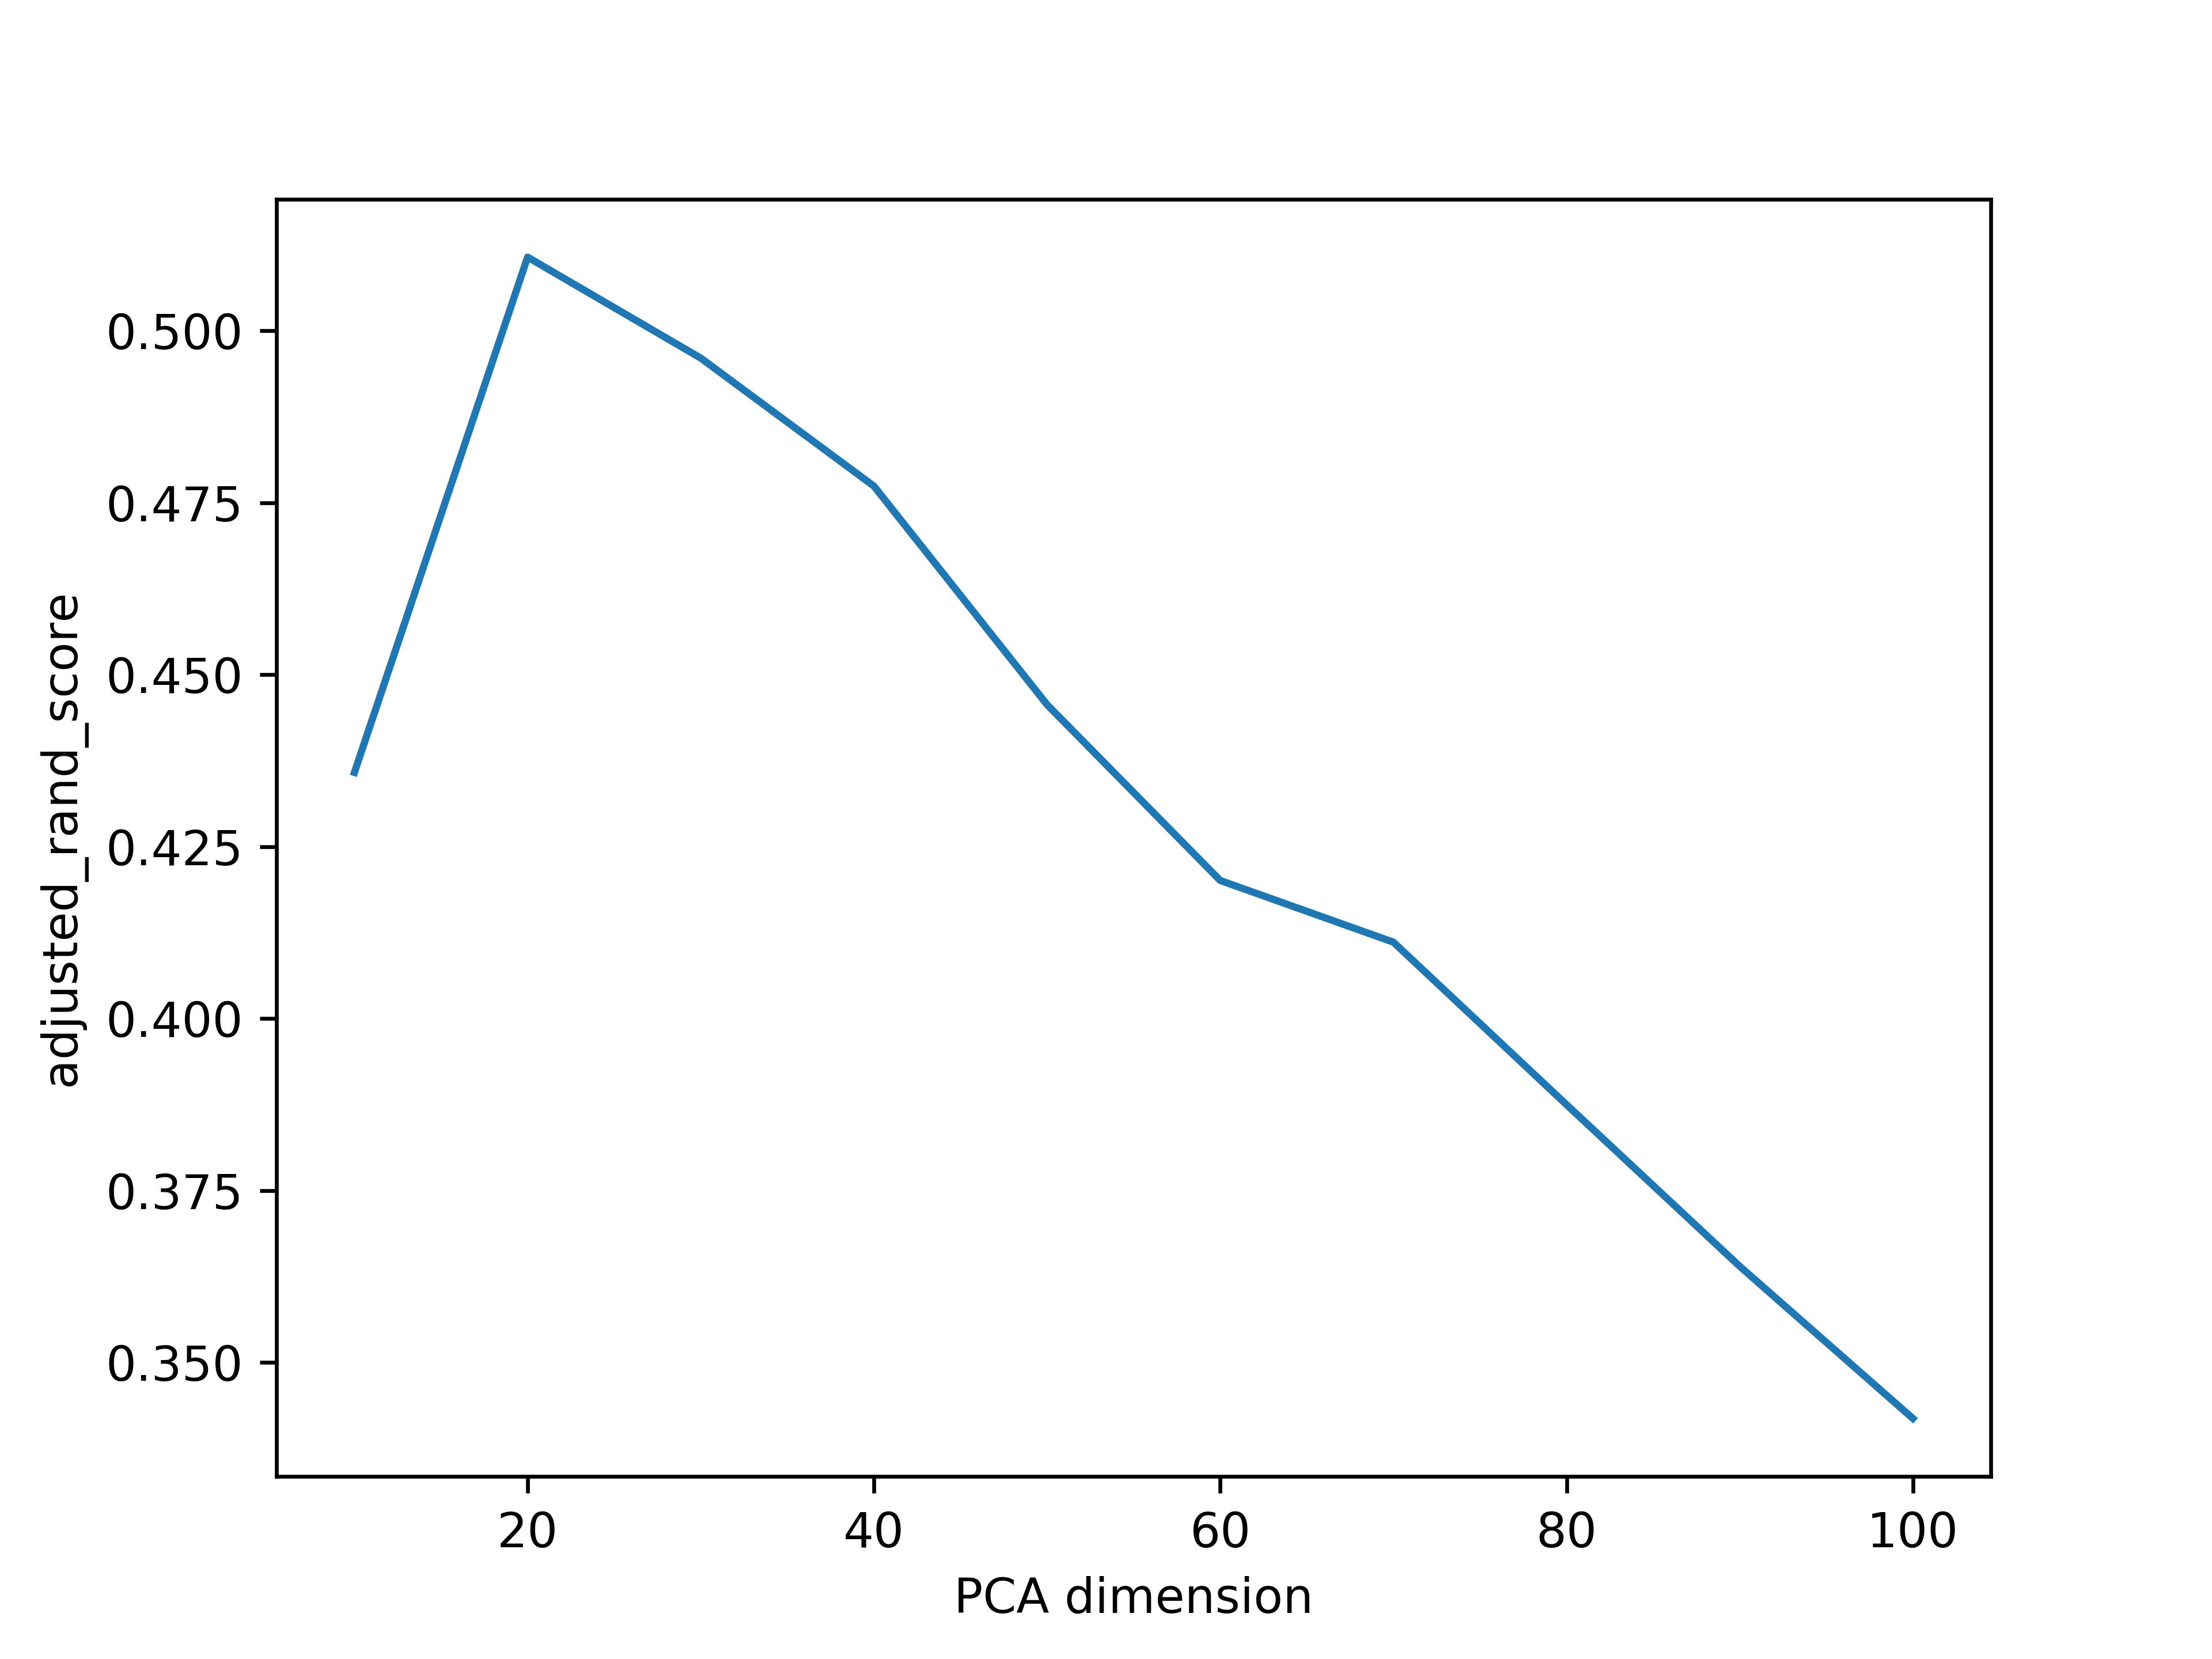
\includegraphics[width=0.5\textwidth]{./figures/cluster_adjusted_rand_score.png}
  \centering
  \caption{$Adjusted~rand~index$随d的变化图}
  \label{cluster_adjusted_rand_score}
\end{figure}

\begin{figure}[!h]
  \centering
   \subfigure[]{
     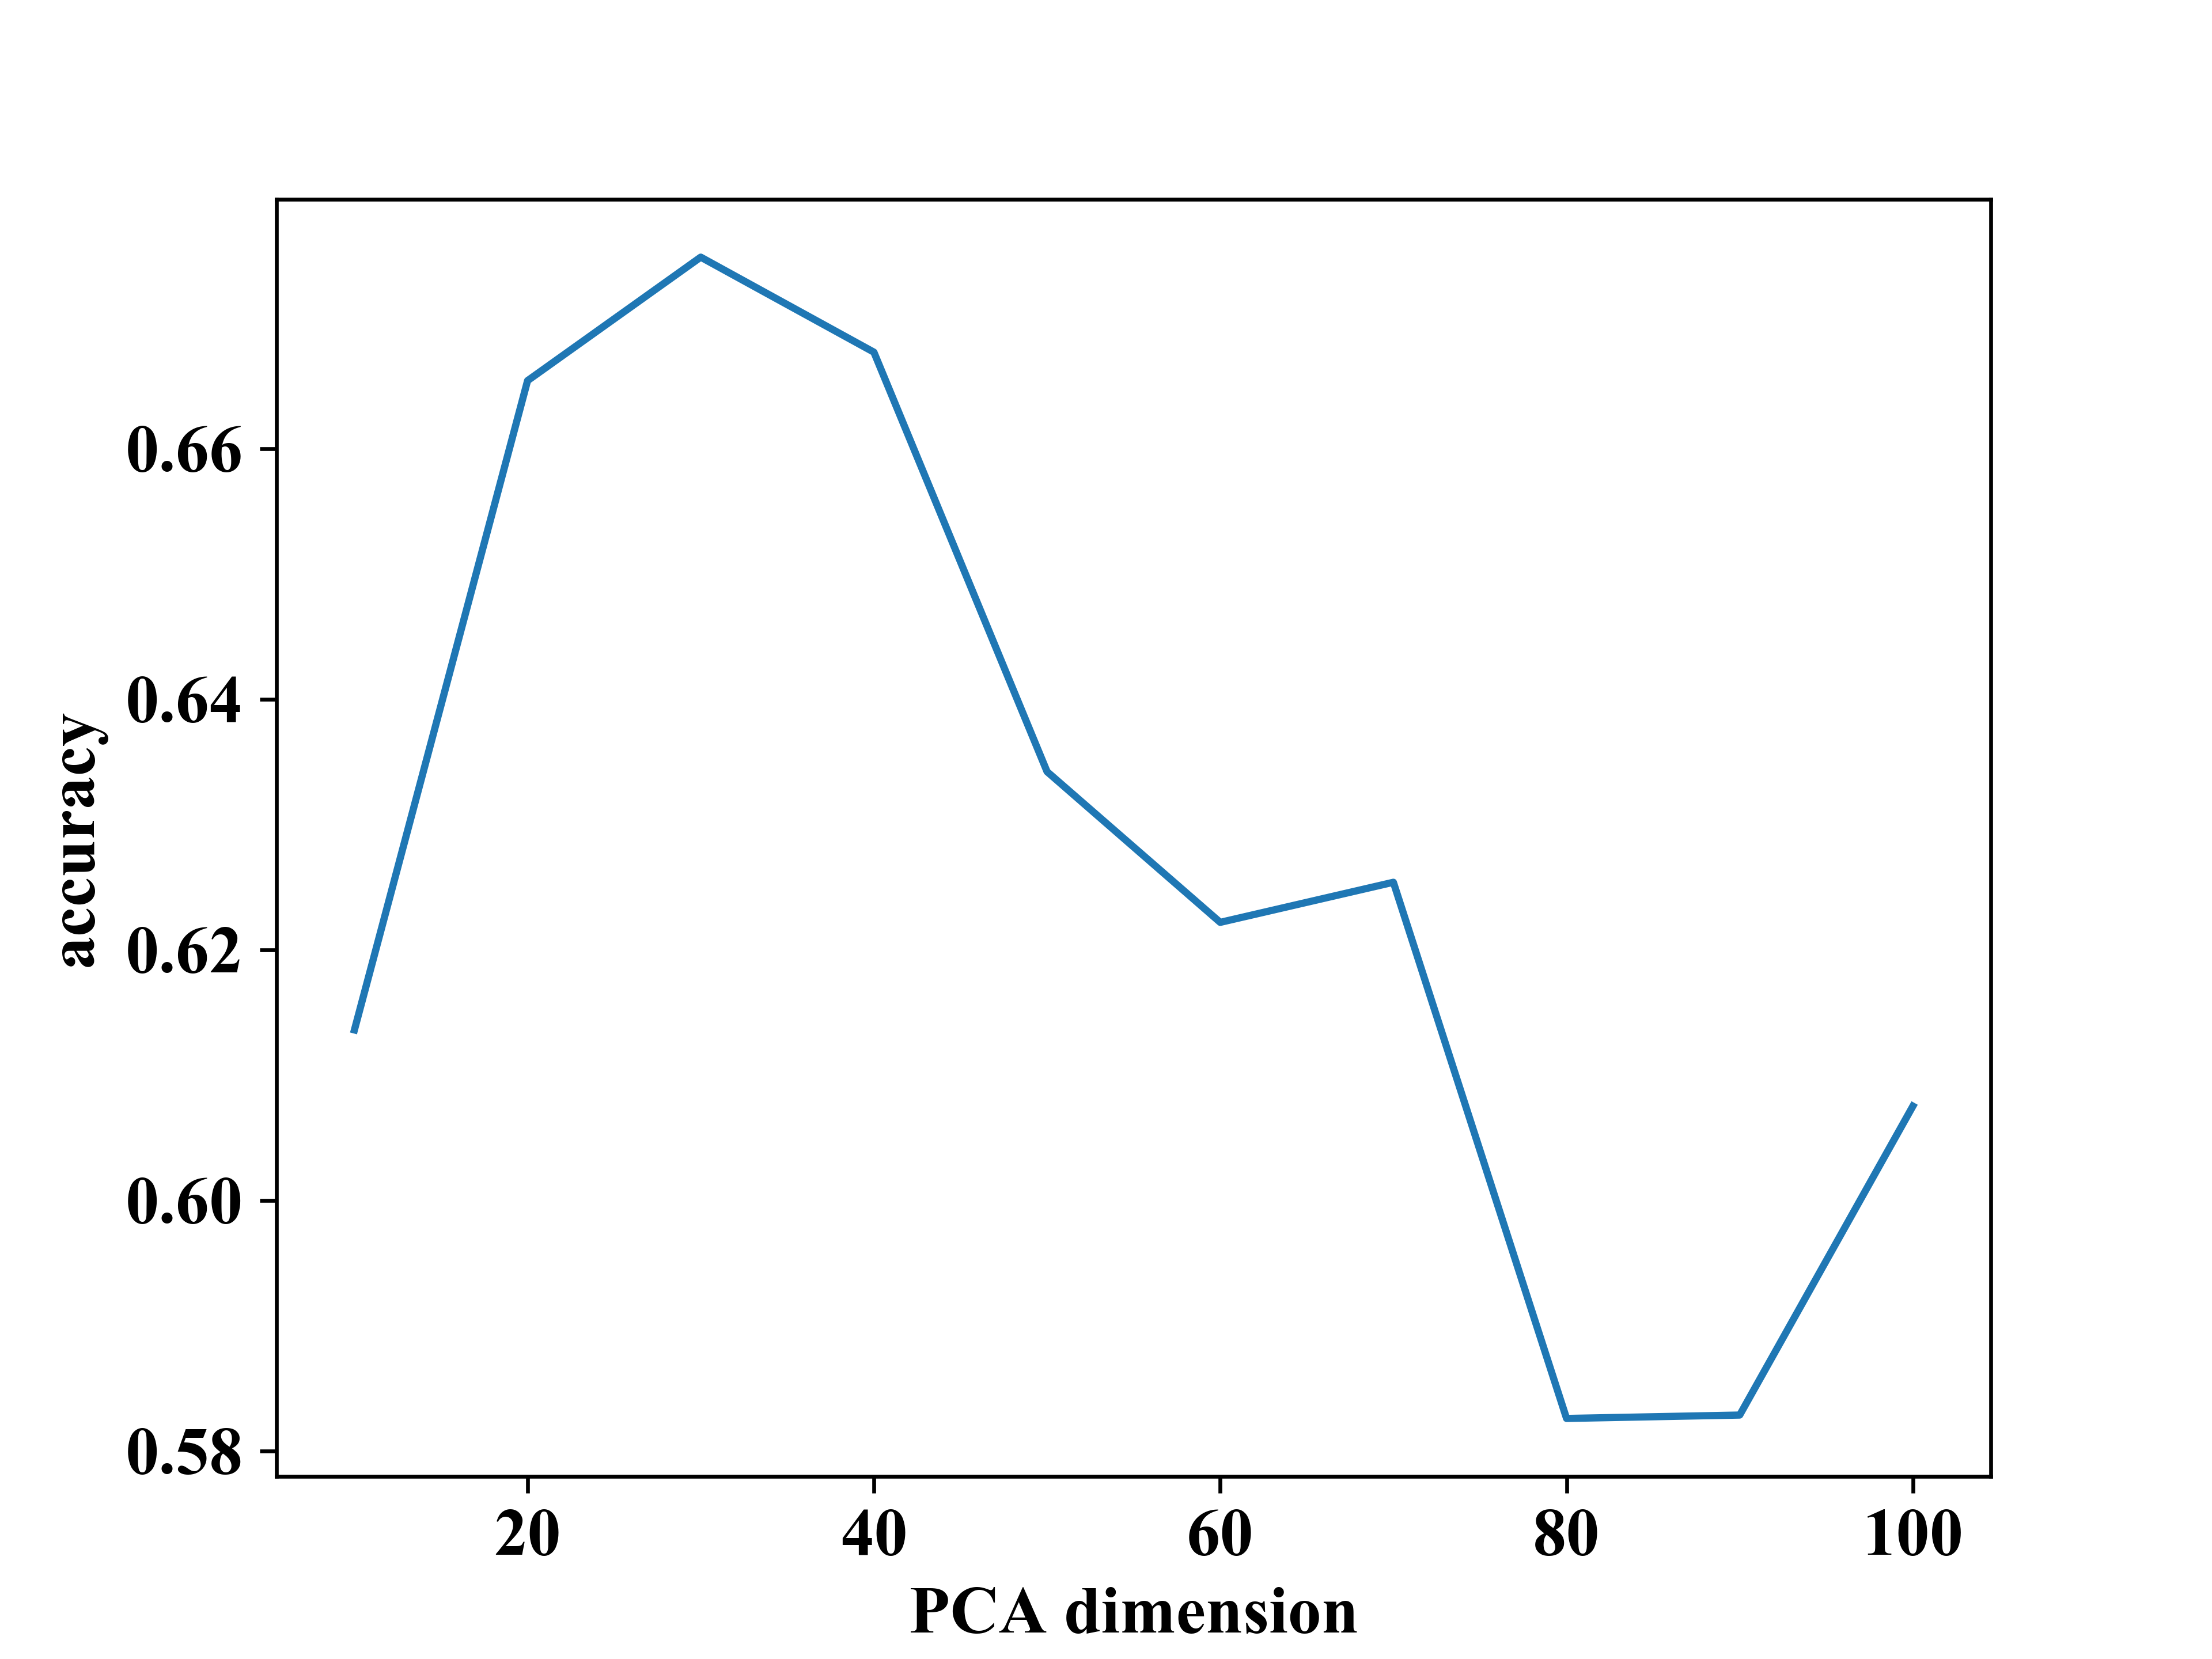
\includegraphics[width=0.45\textwidth]{figures/cluster_acc.png}\label{fig:cluster_acc}
   }\quad
   \subfigure[]{
     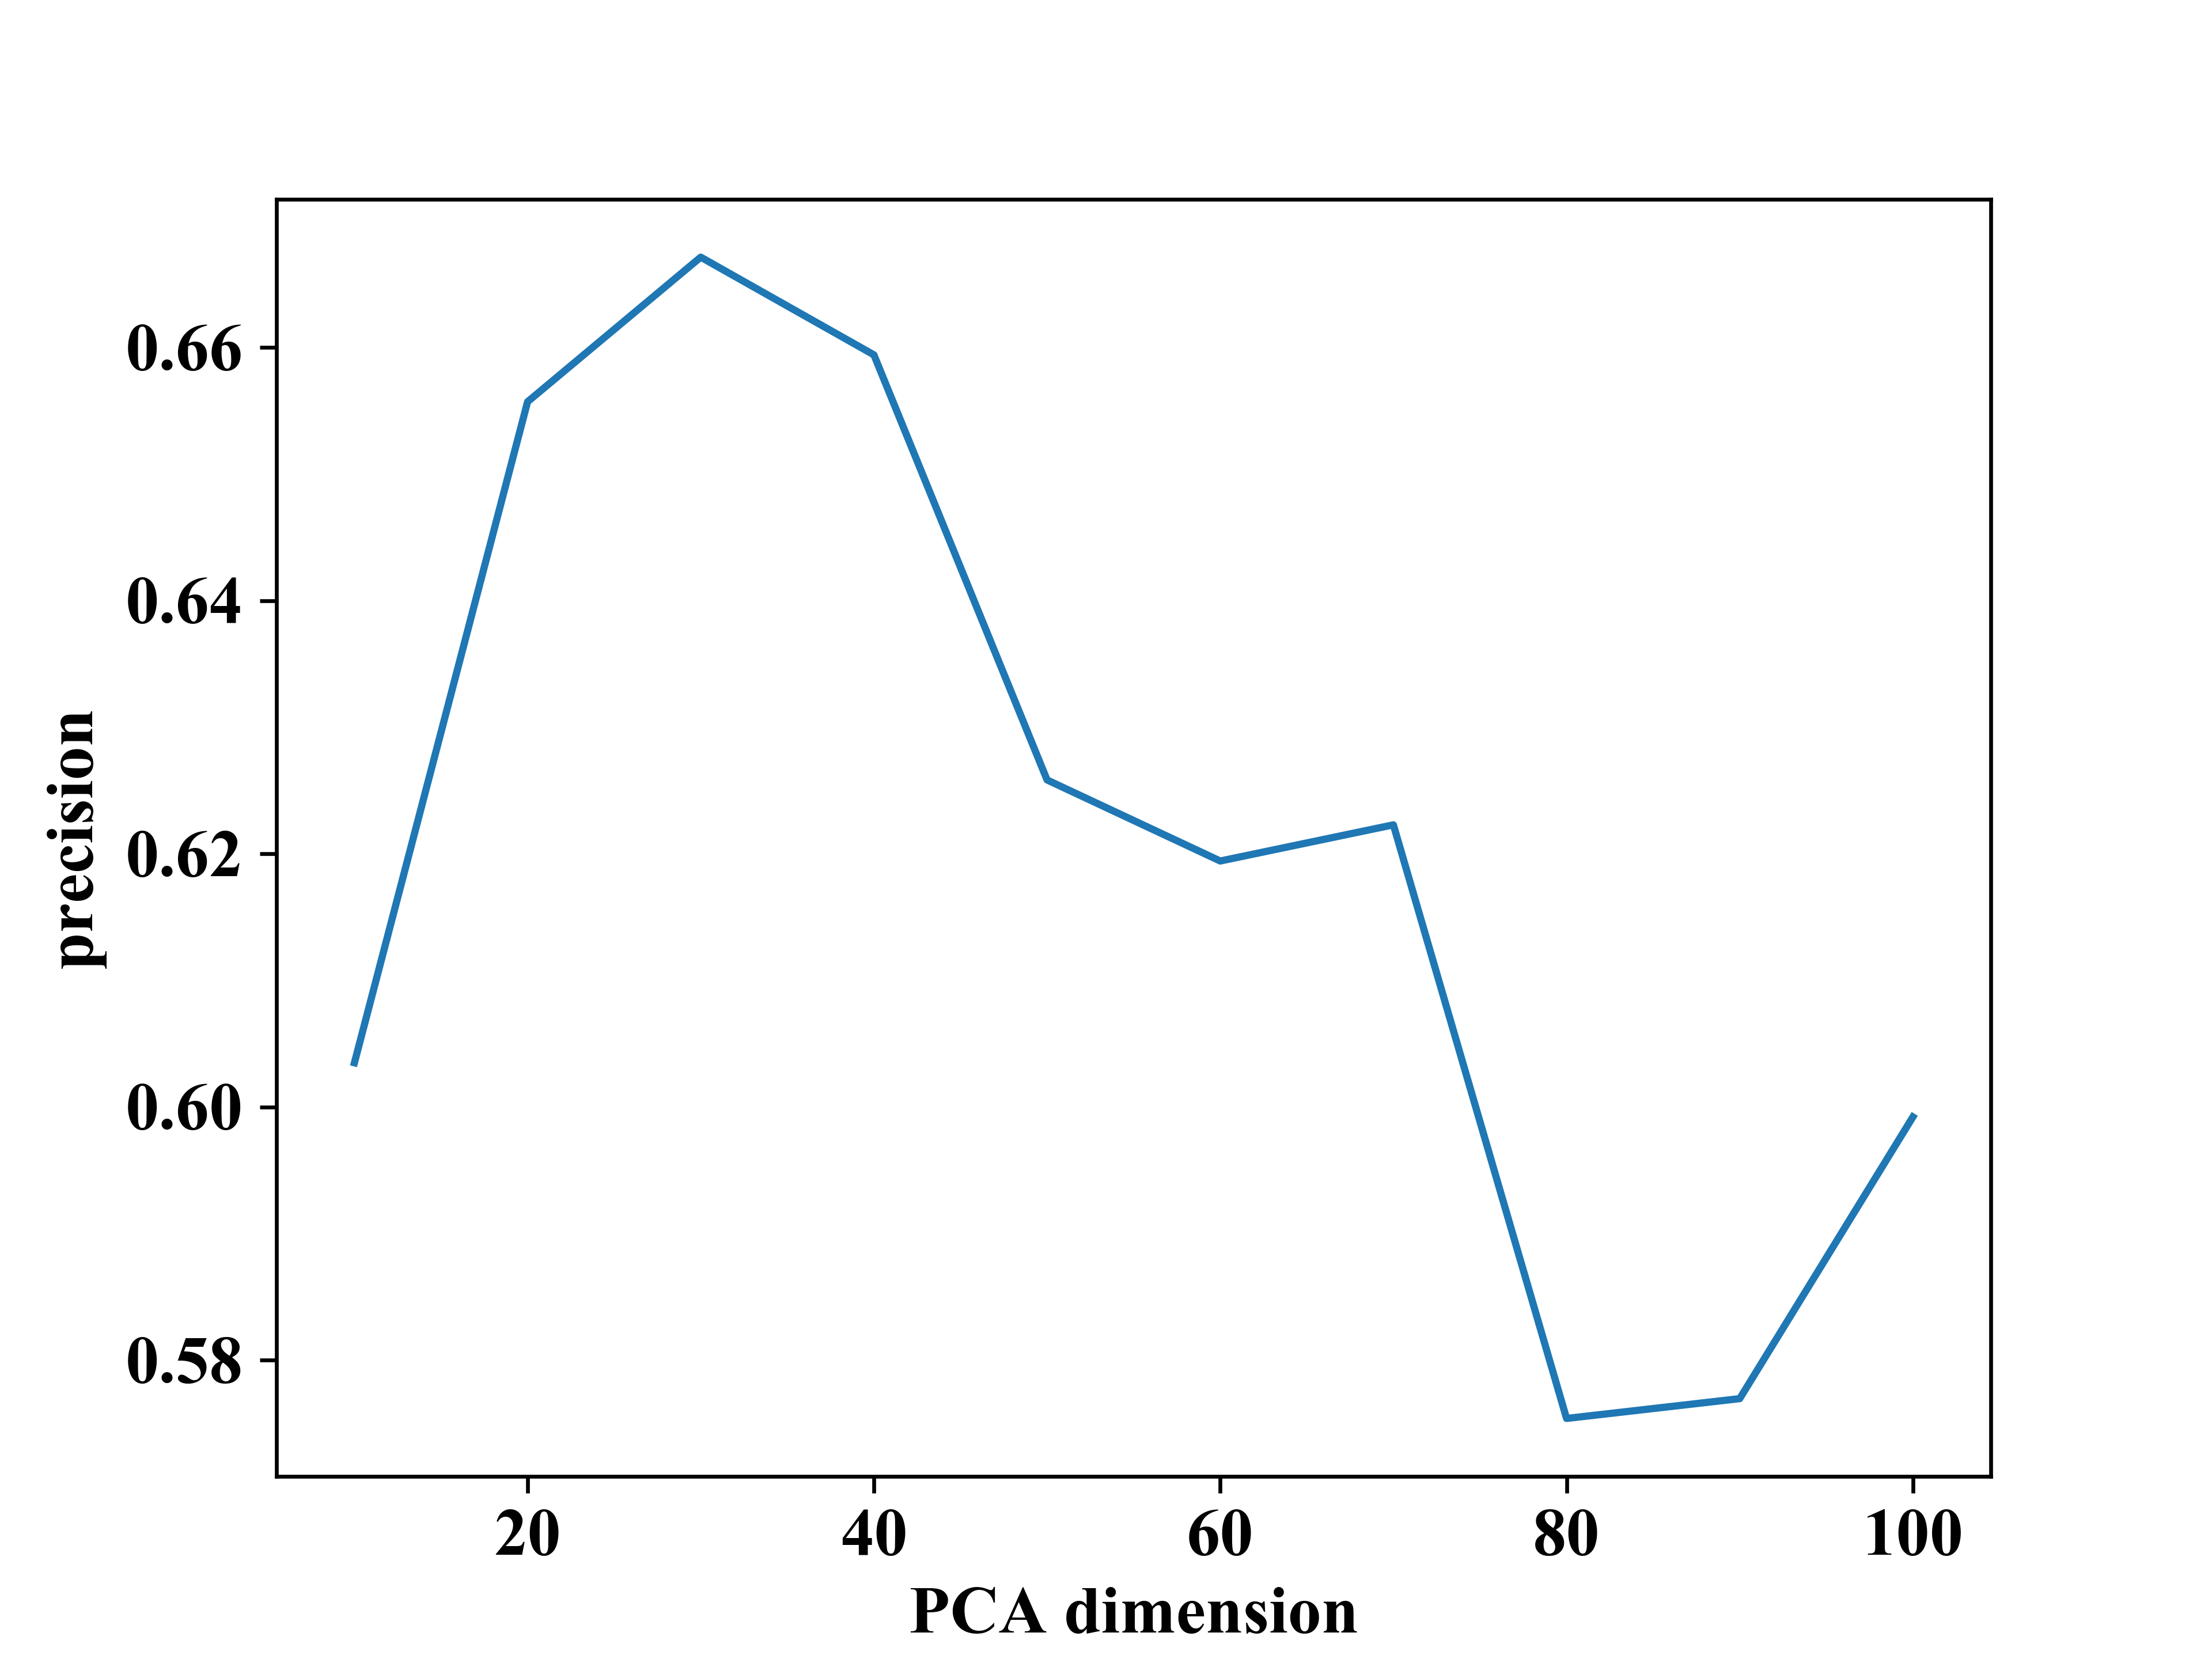
\includegraphics[width=0.45\textwidth]{figures/cluster_precision.png}\label{fig:cluster_precision}
   }\quad
   \subfigure[]{
     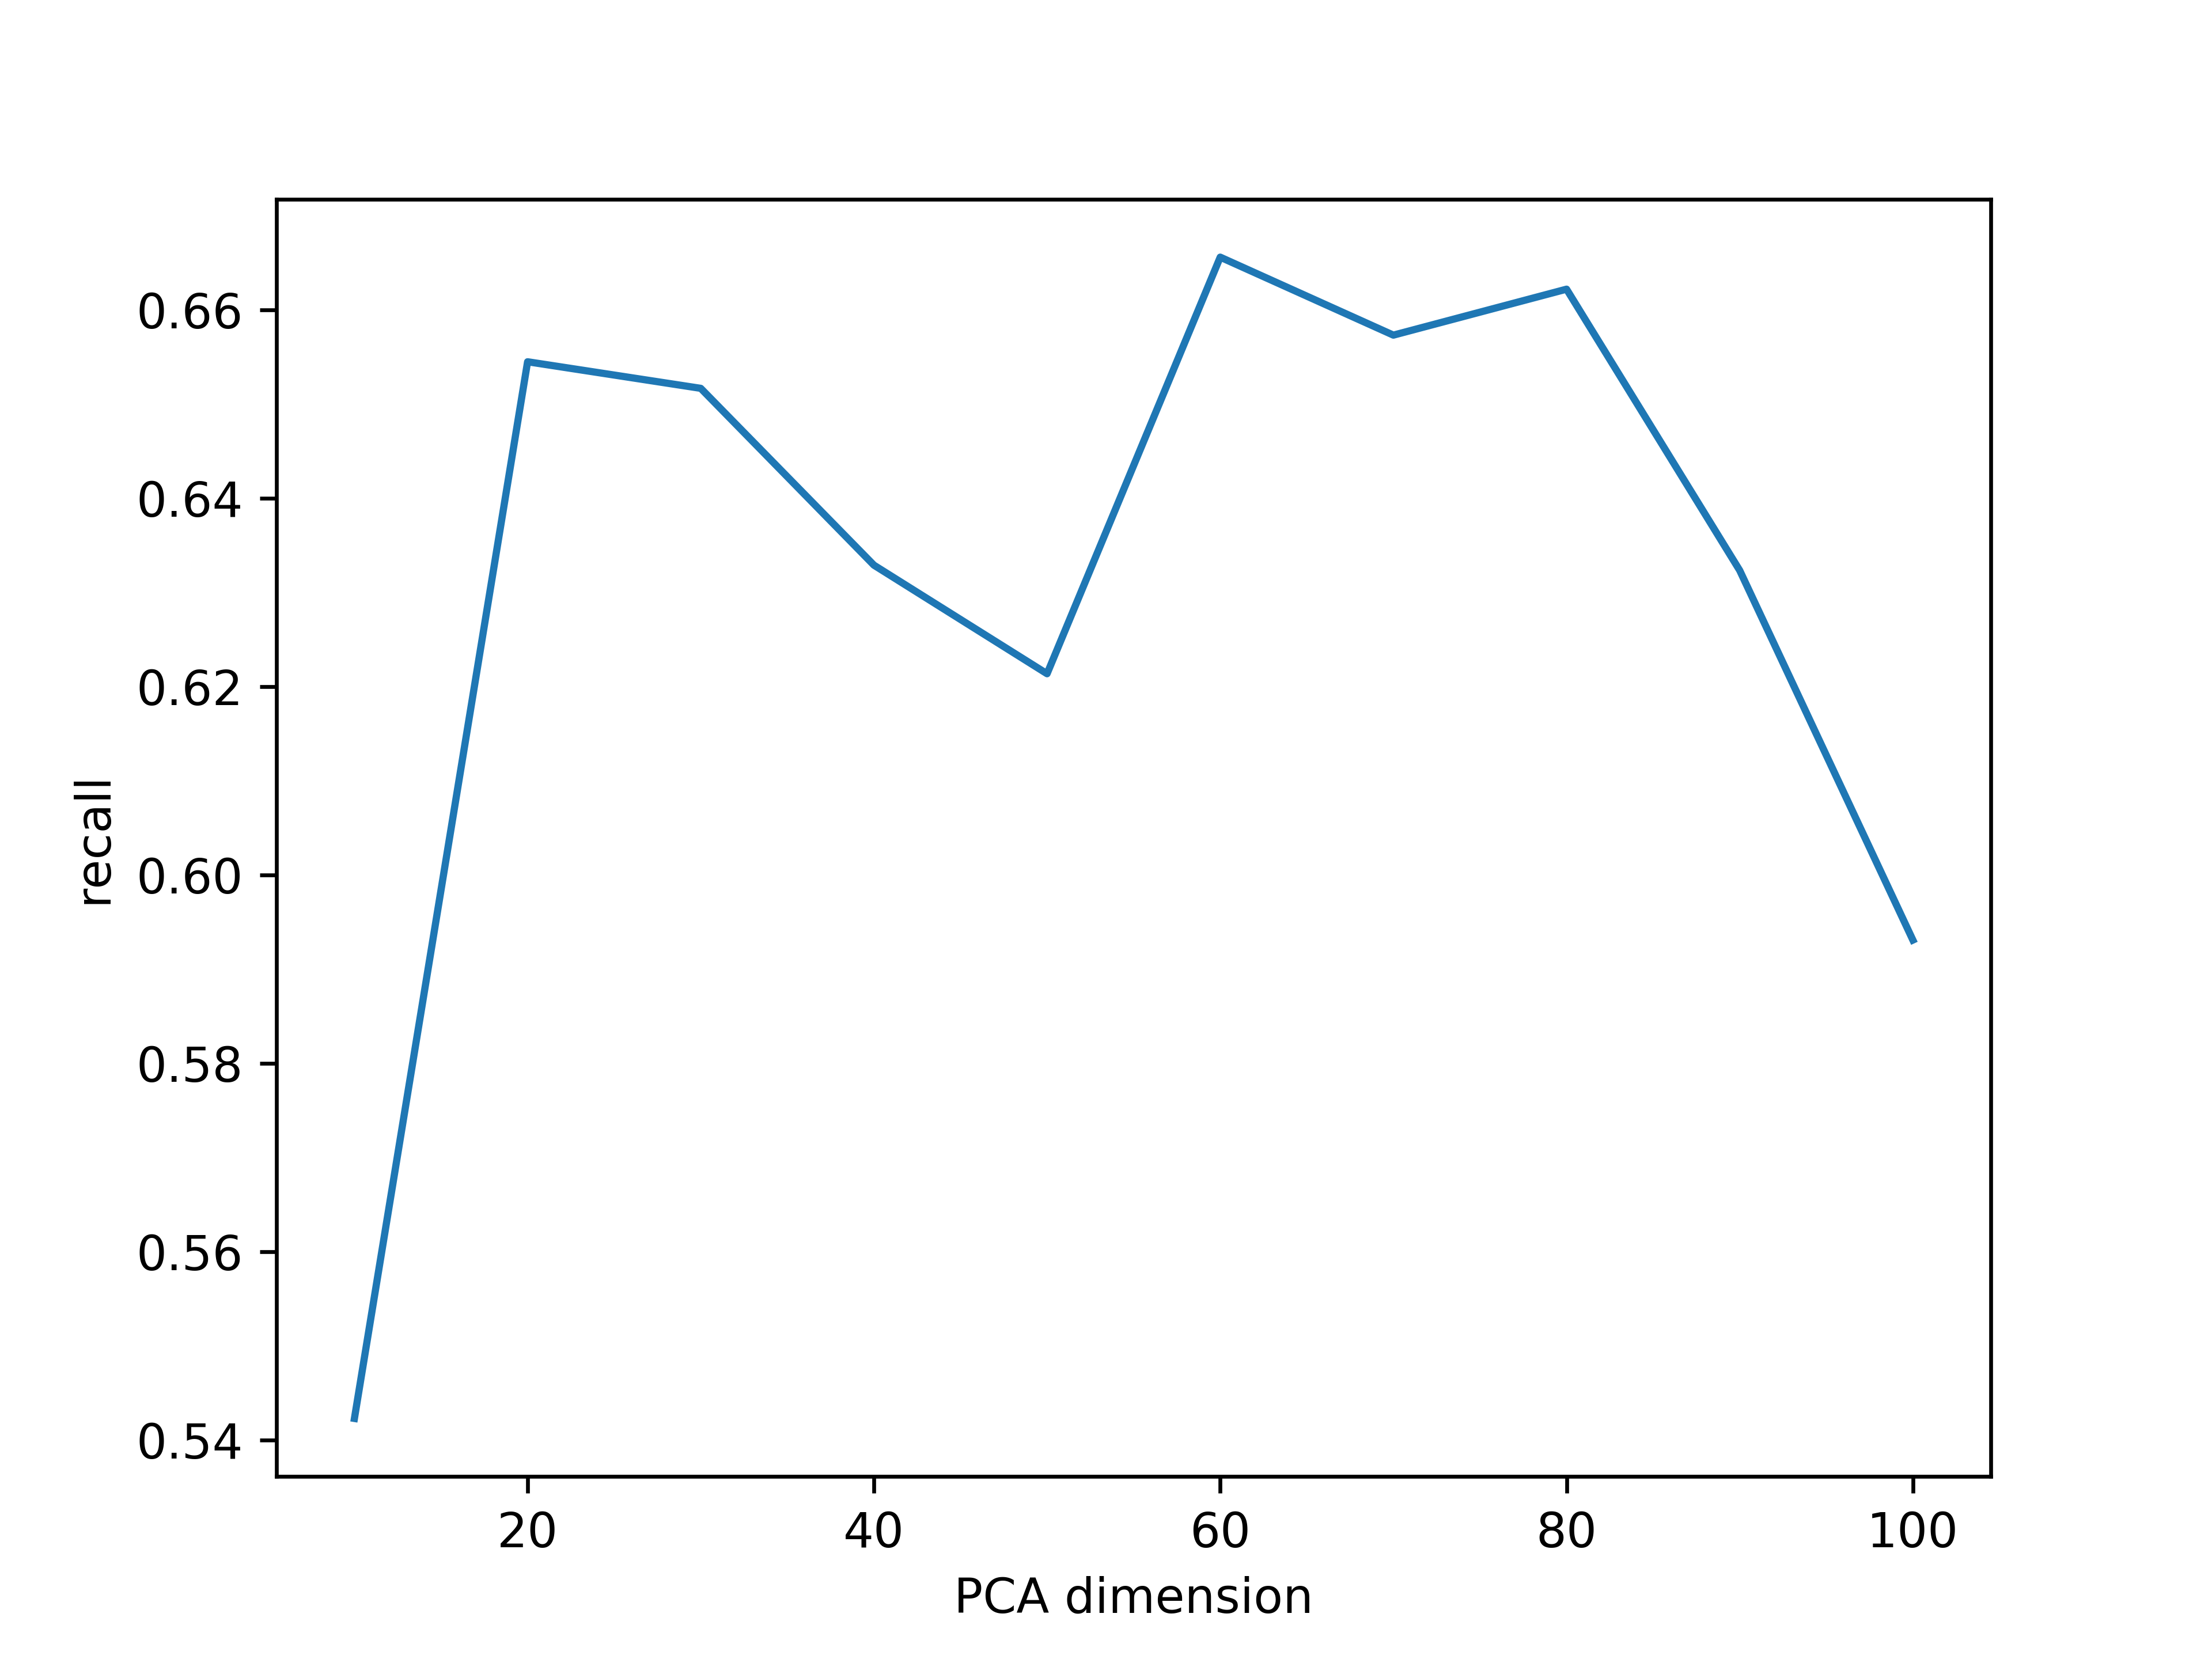
\includegraphics[width=0.45\textwidth]{figures/cluster_recall.png}\label{fig:cluster_recall}
   }\quad  
   \subfigure[]{
     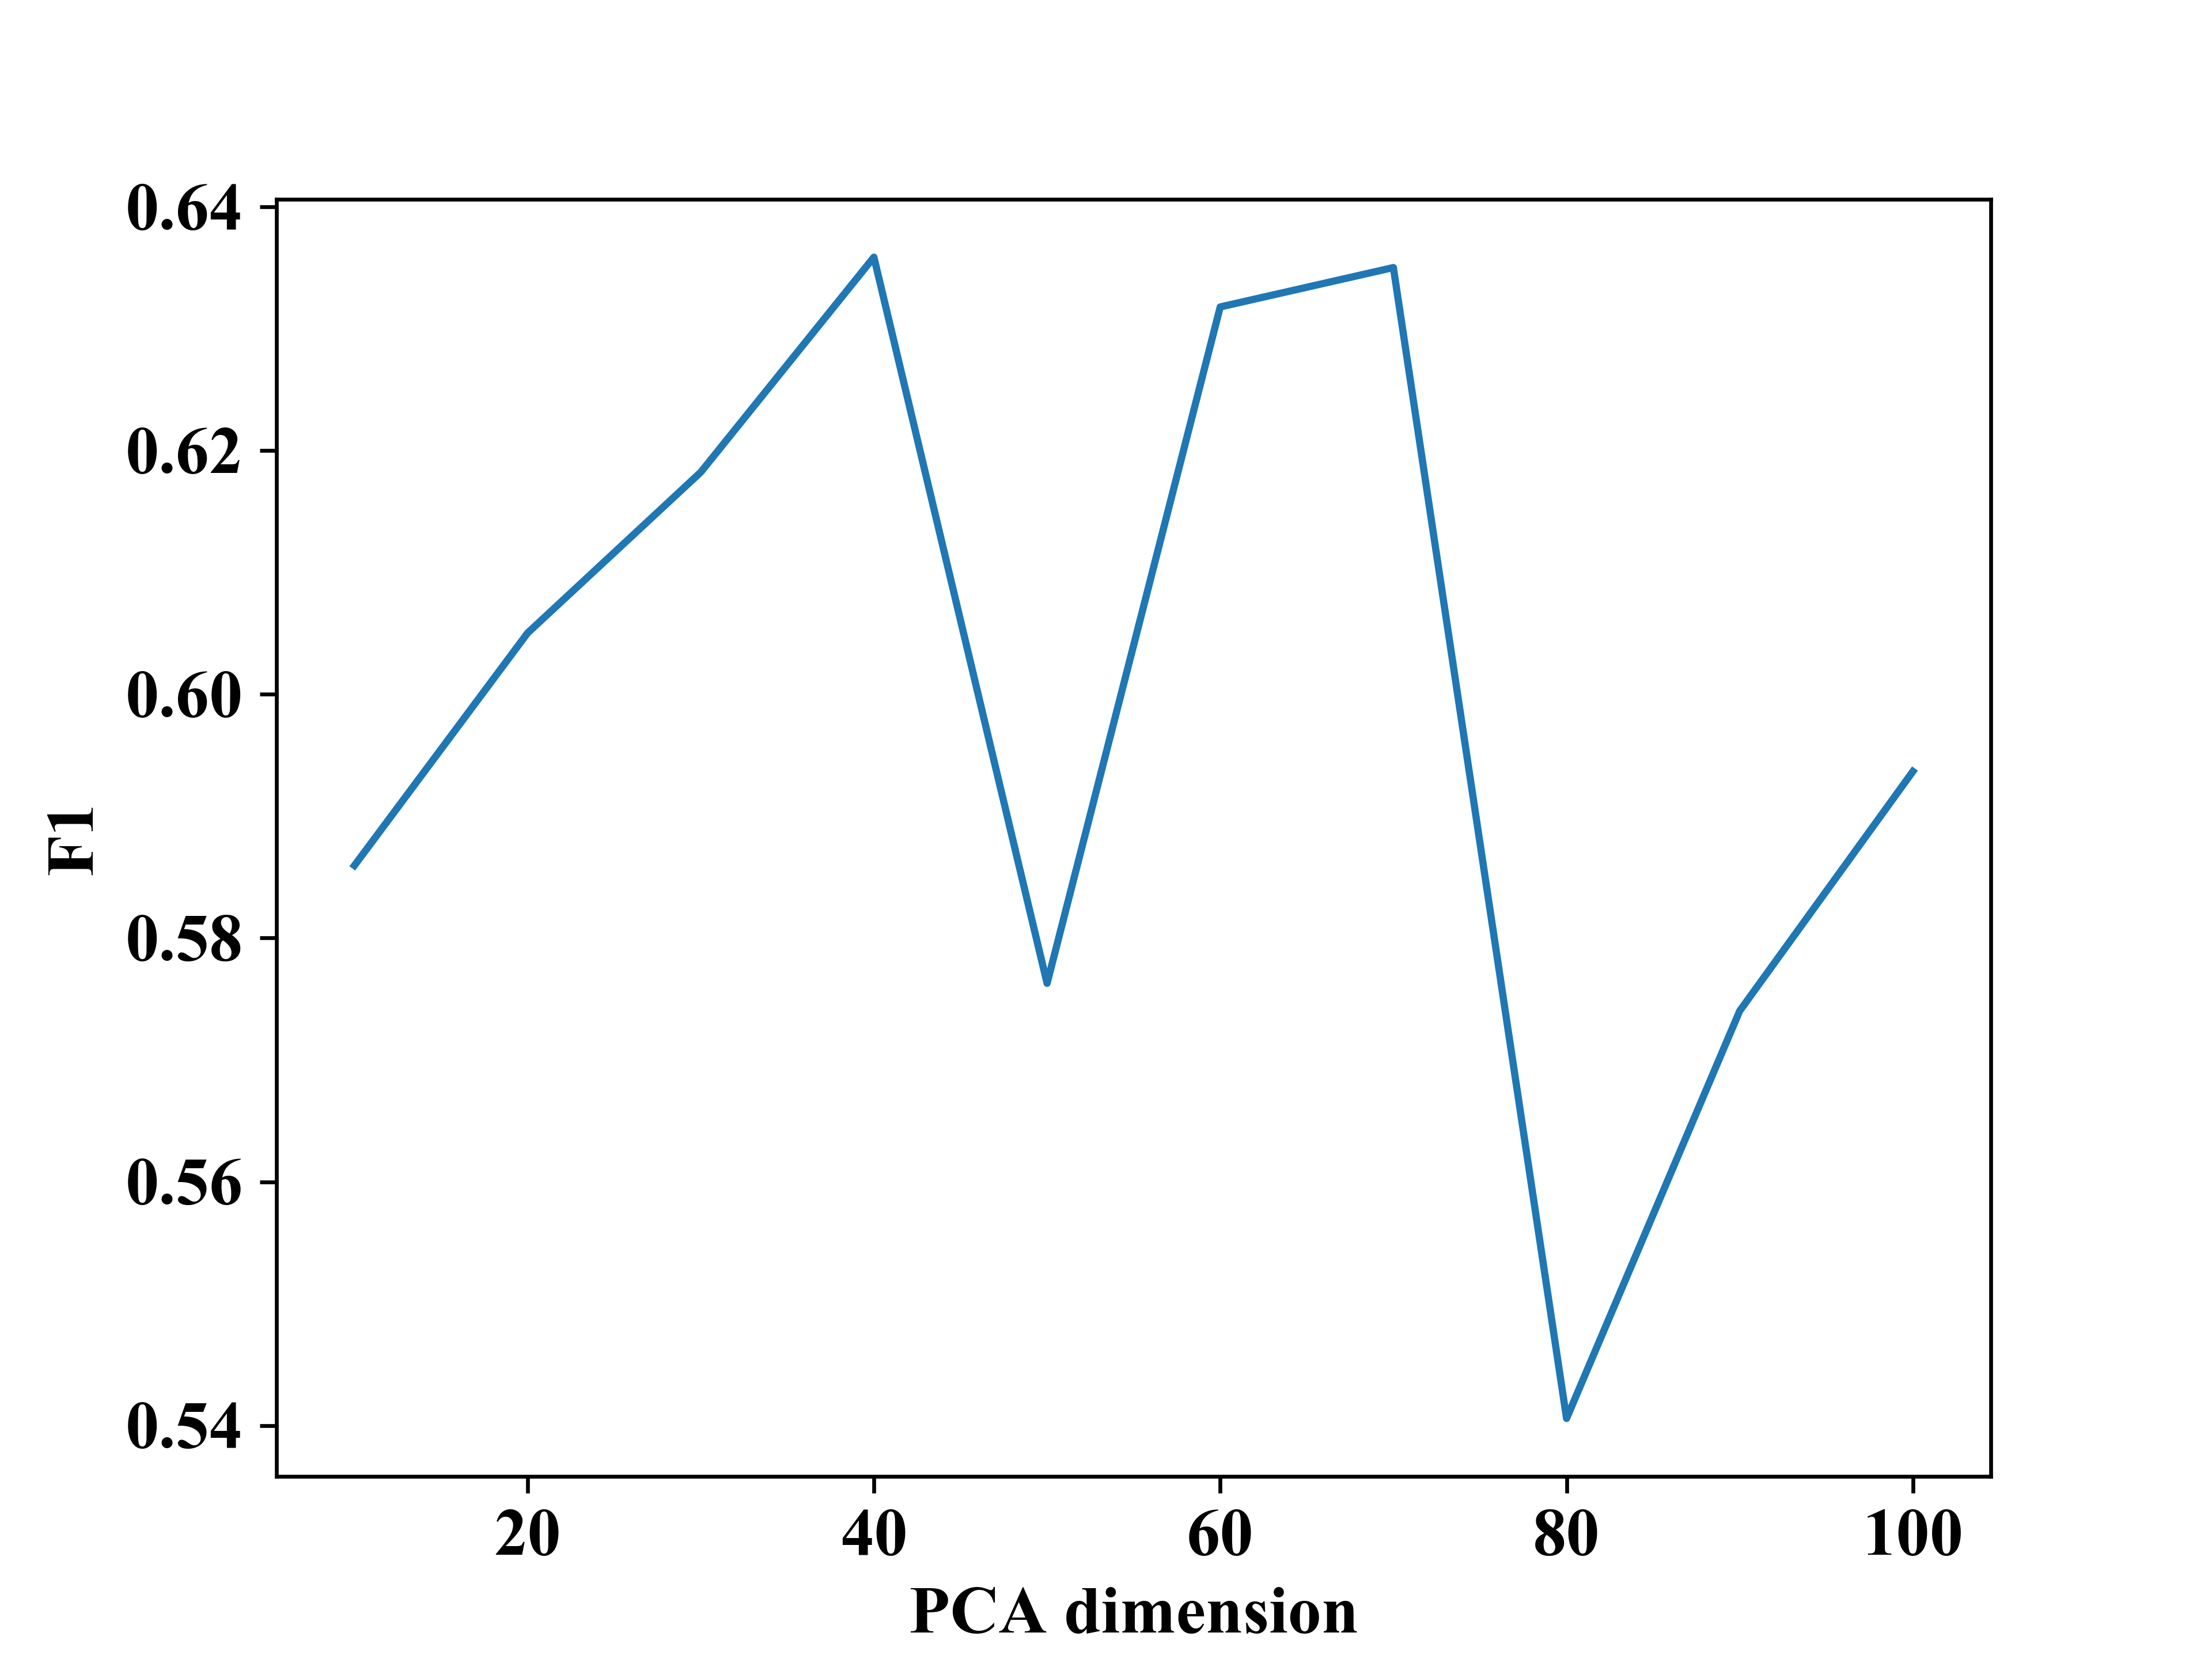
\includegraphics[width=0.45\textwidth]{figures/cluster_f1.png}\label{fig:cluster_f1}
   }
  \caption{其它指标随d的变化图}\label{fig:cluster_metrics}
\end{figure}

\begin{figure}[!h]
  \includegraphics[width=0.8\textwidth]{./figures/GMM_means.png}
  \centering
  \caption{GMM聚类中心点可视化}
  \label{GMM_means}
\end{figure}

我们把PCA降维的维度$d$作为横轴,分别把$Adjusted~rand~index$,$accuracy$,$precision$,$recall$,$F1$这些评价标准作为纵轴,将其结果可视化出来,如下图~\ref{cluster_adjusted_rand_score},~\ref{fig:cluster_metrics}所示。

% \begin{figure}[!h]
%   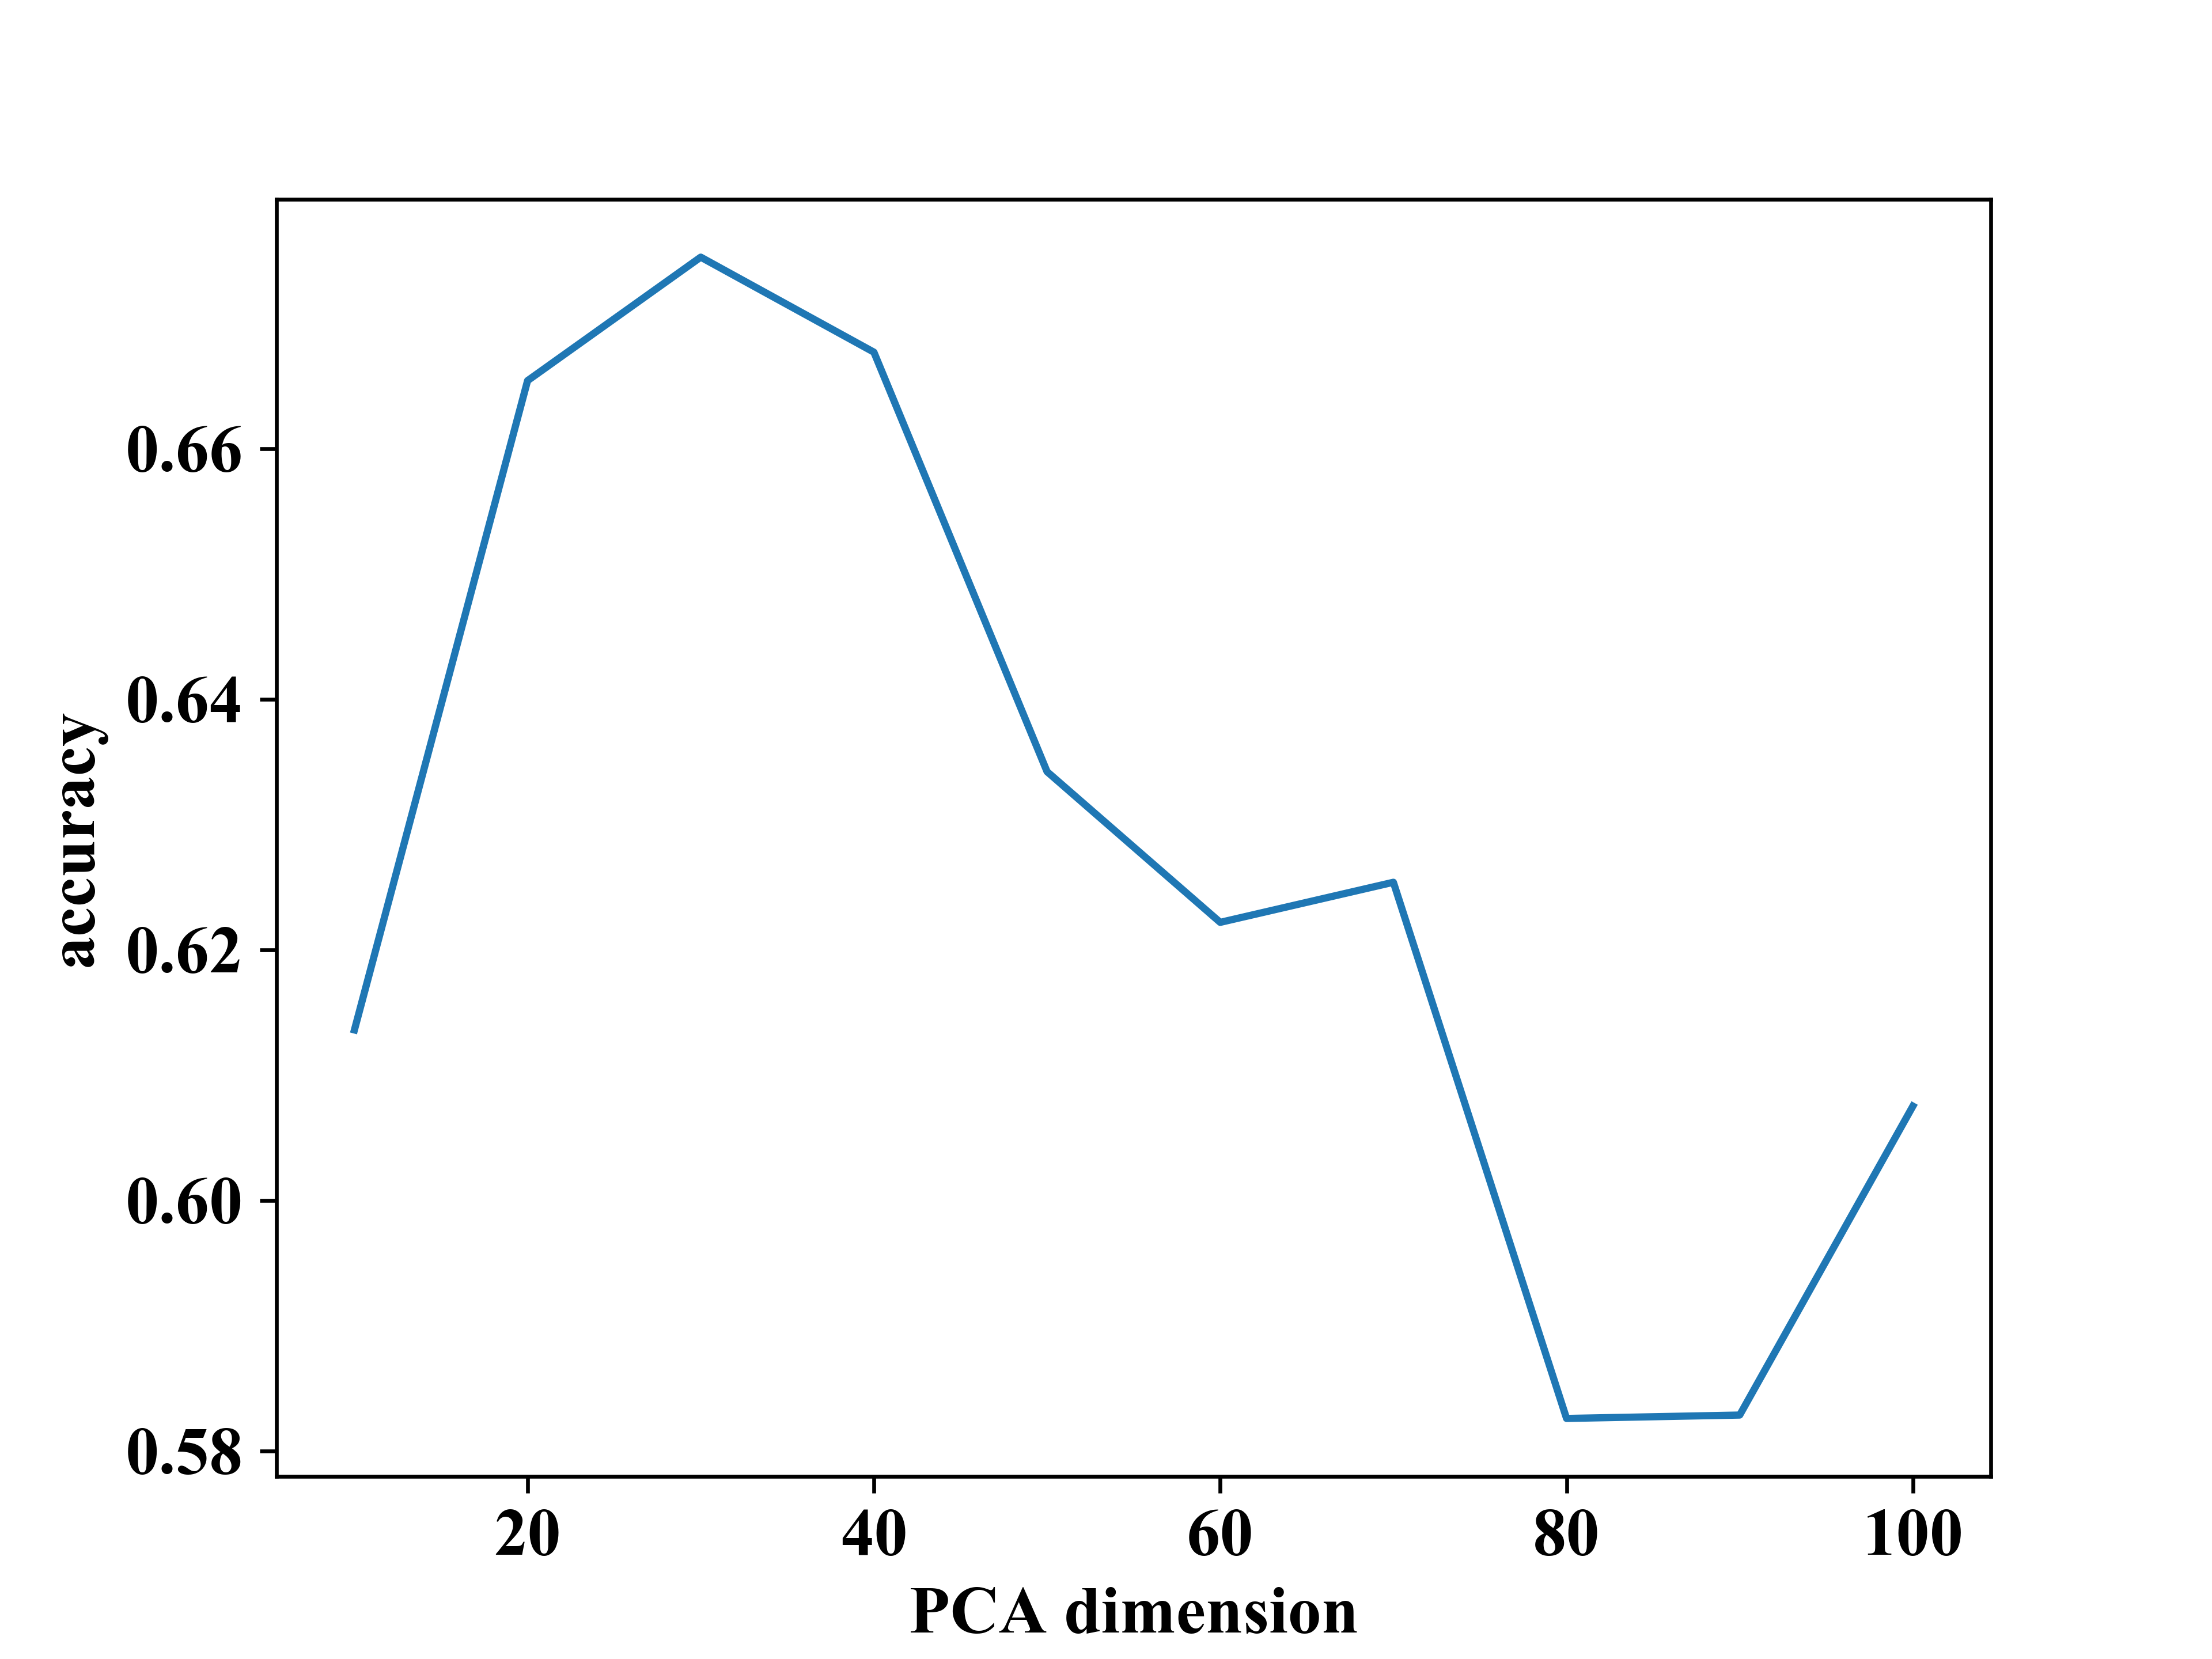
\includegraphics[width=0.5\textwidth]{./figures/cluster_acc.png}
%   \centering
%   \caption{acc随d的变化图}
%   \label{cluster_acc}
% \end{figure}


% \begin{figure}[!h]
%   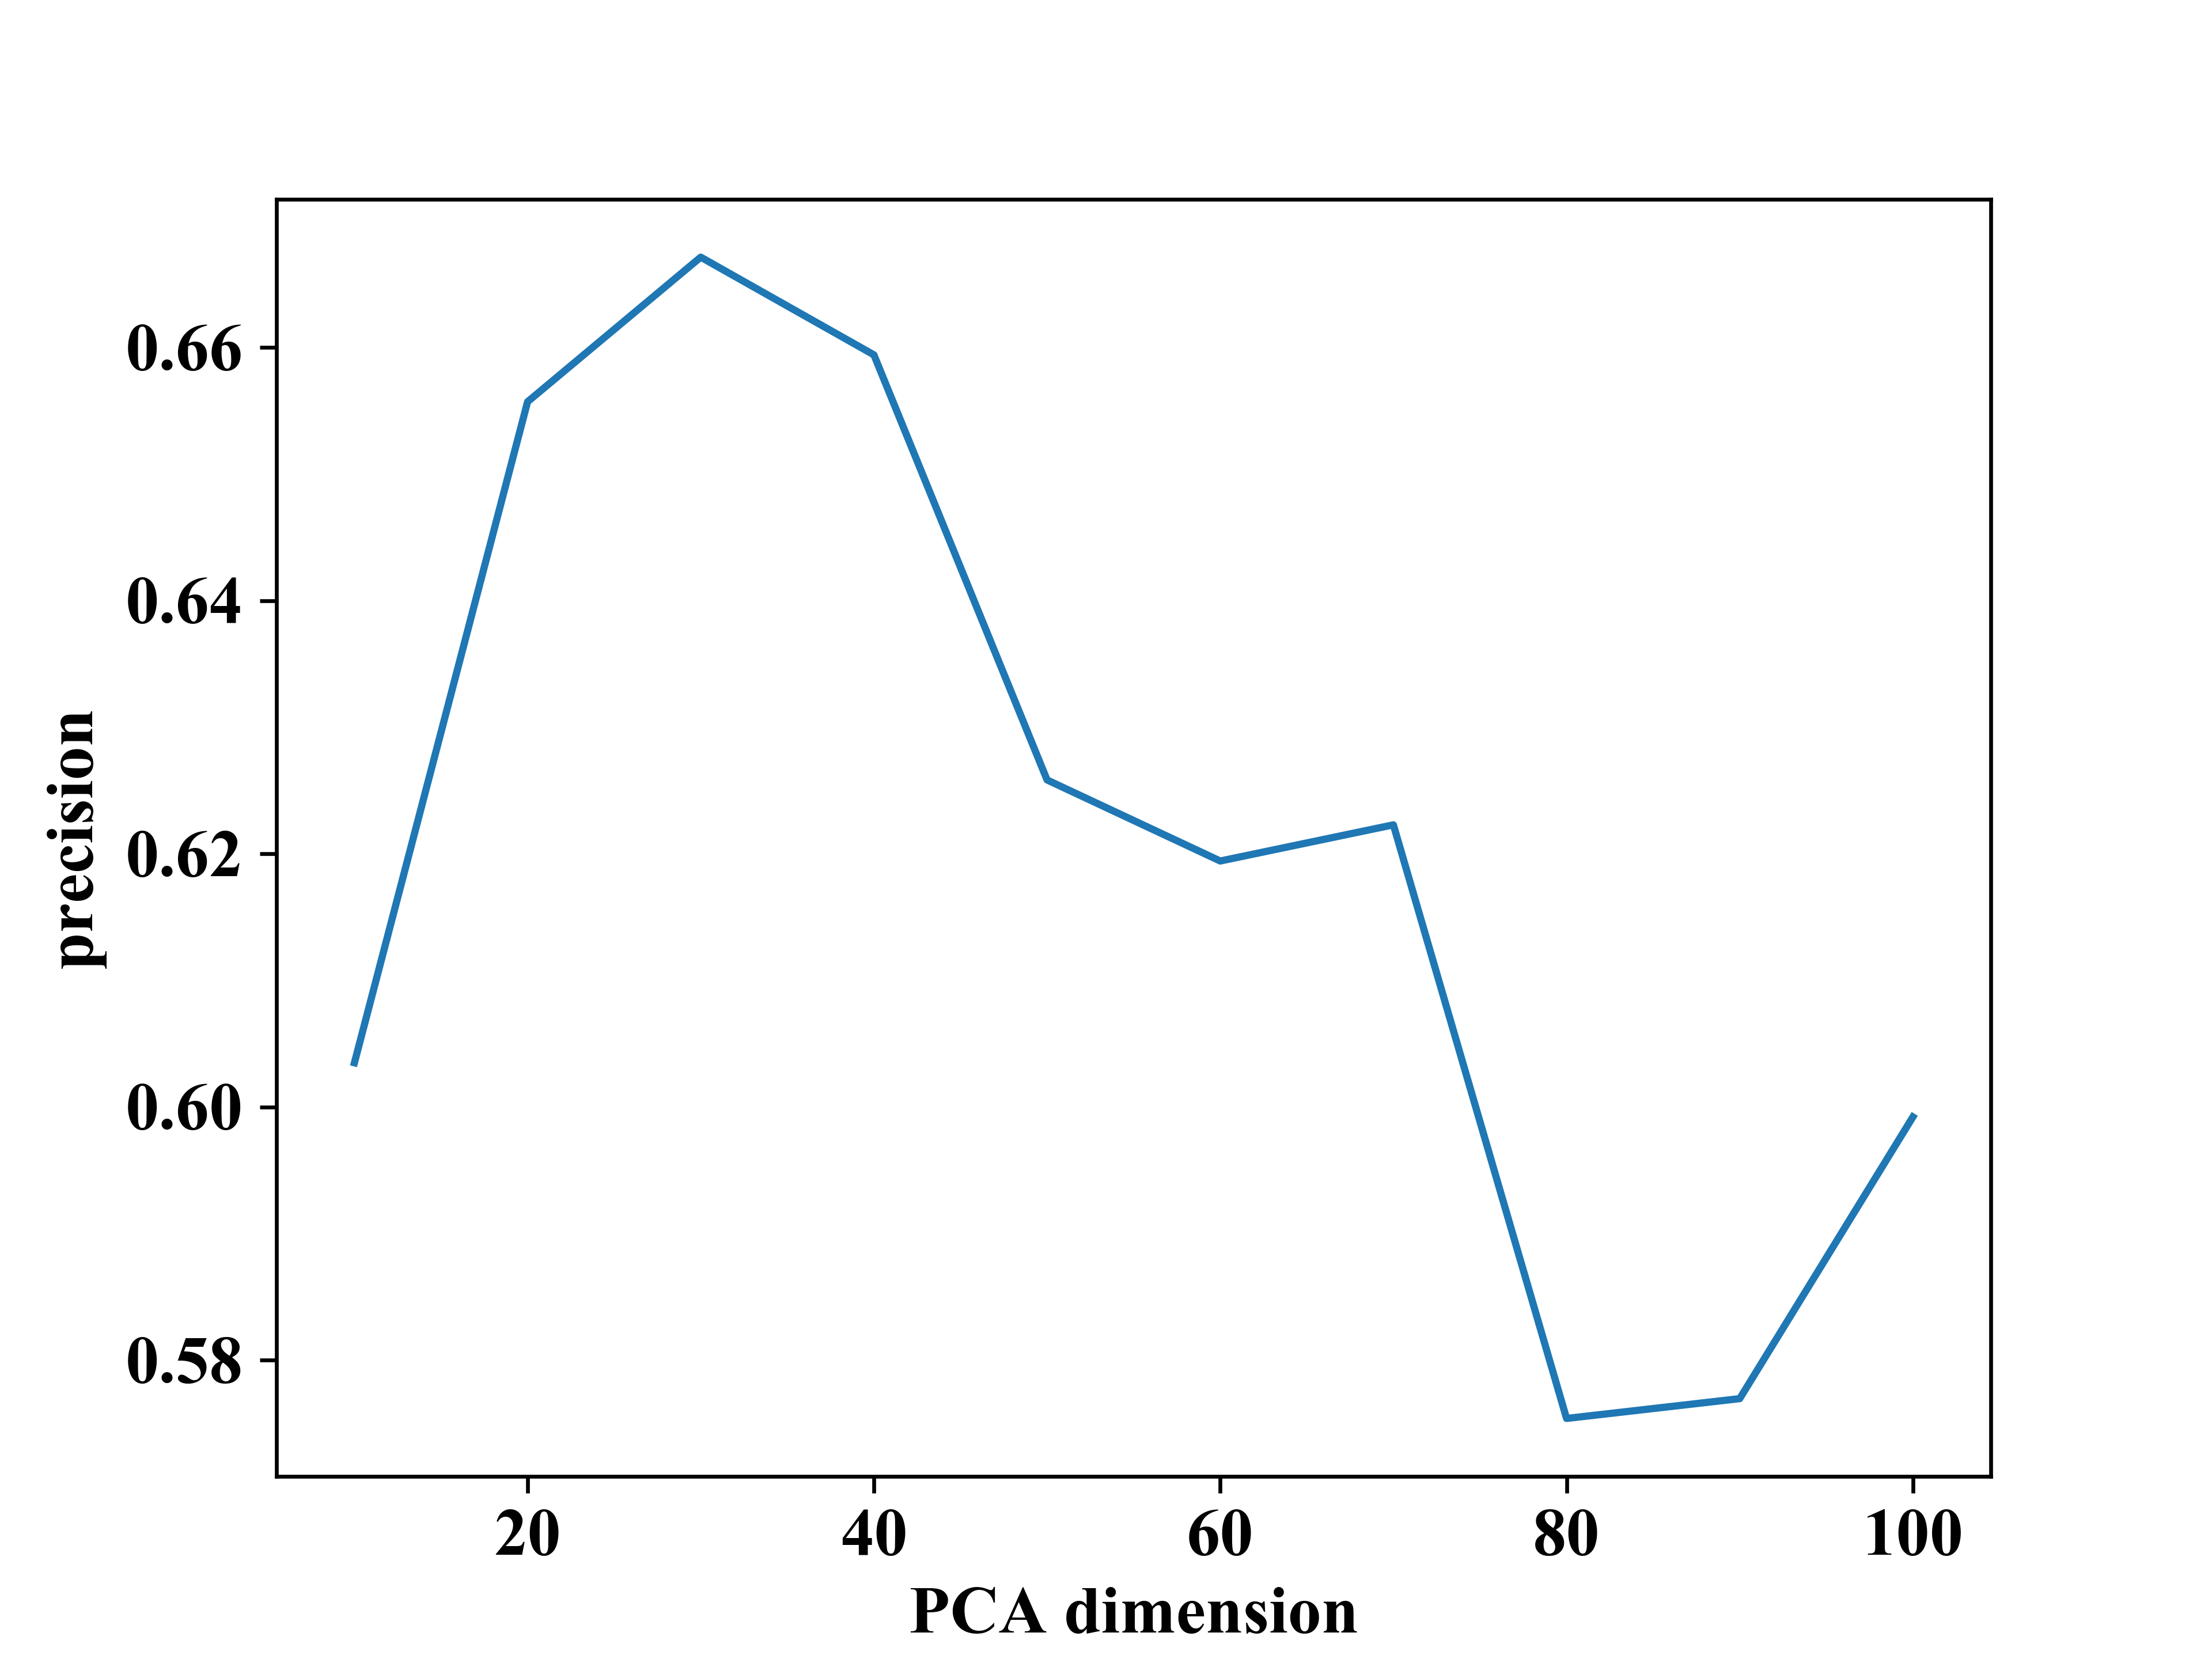
\includegraphics[width=0.5\textwidth]{./figures/cluster_precision.png}
%   \centering
%   \caption{precision随d的变化图}
%   \label{cluster_precision}
% \end{figure}


% \begin{figure}[!h]
%   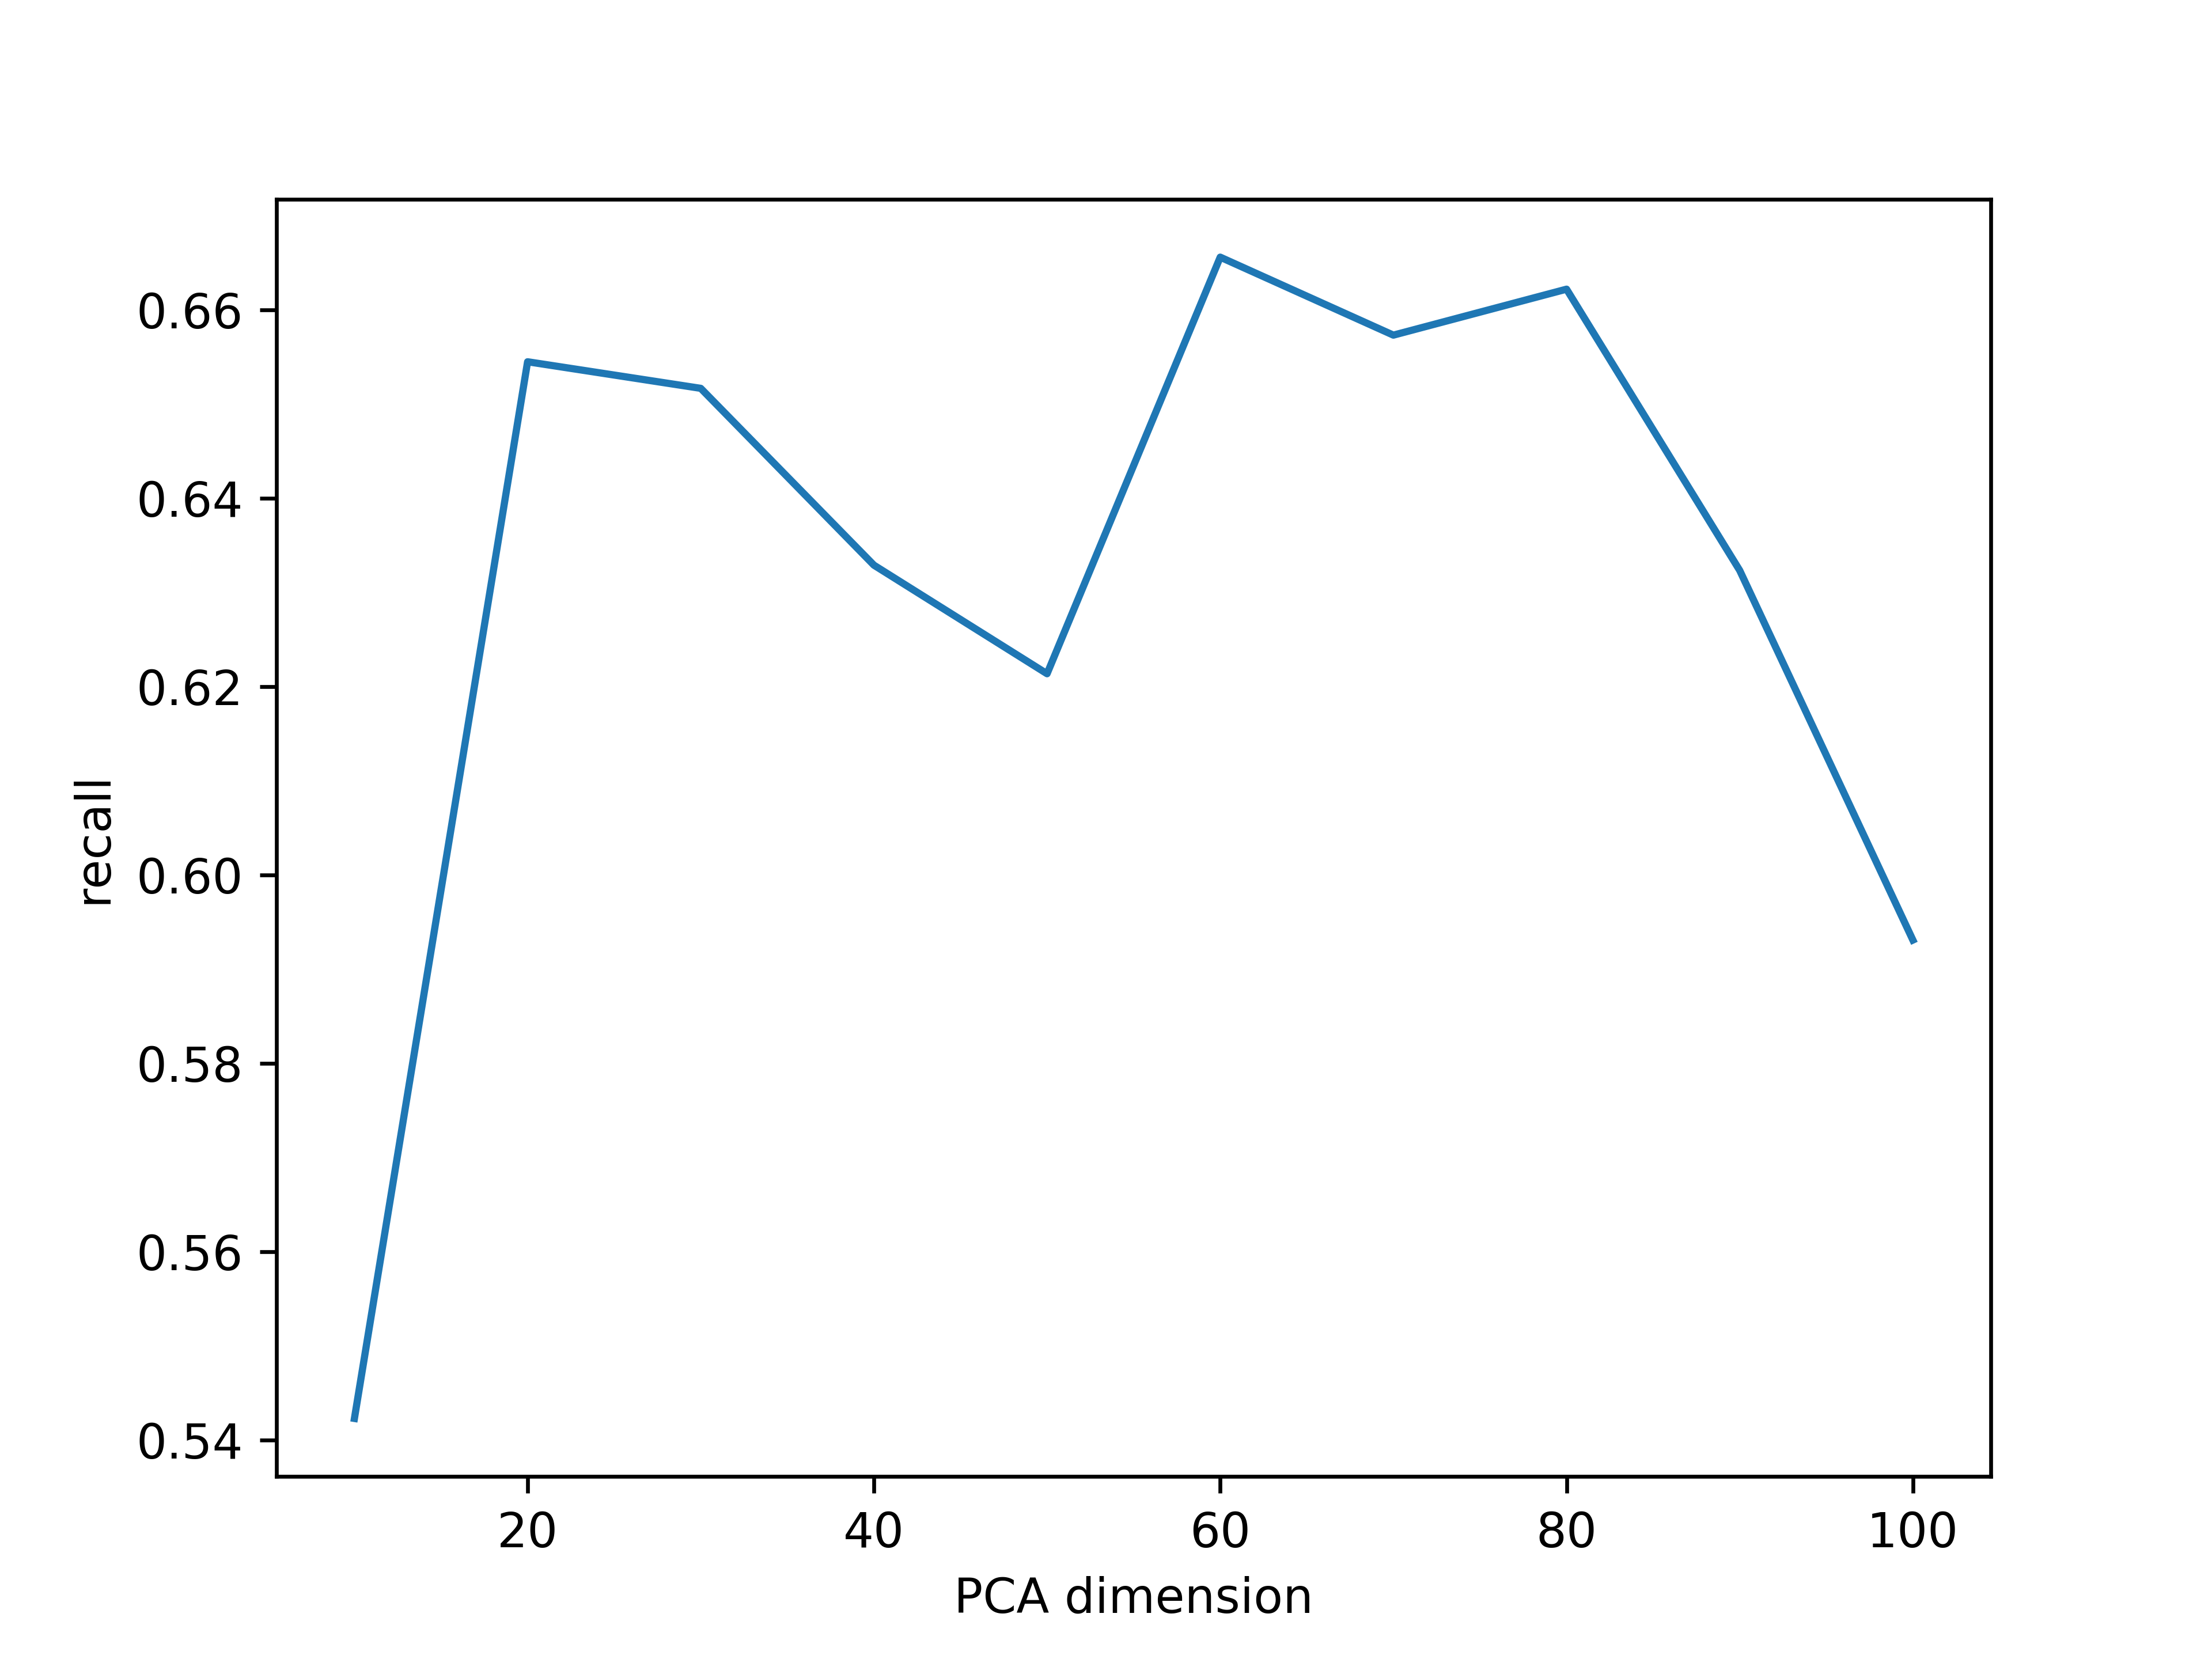
\includegraphics[width=0.5\textwidth]{./figures/cluster_recall.png}
%   \centering
%   \caption{recall随d的变化图}
%   \label{cluster_recall}
% \end{figure}


% \begin{figure}[!h]
%   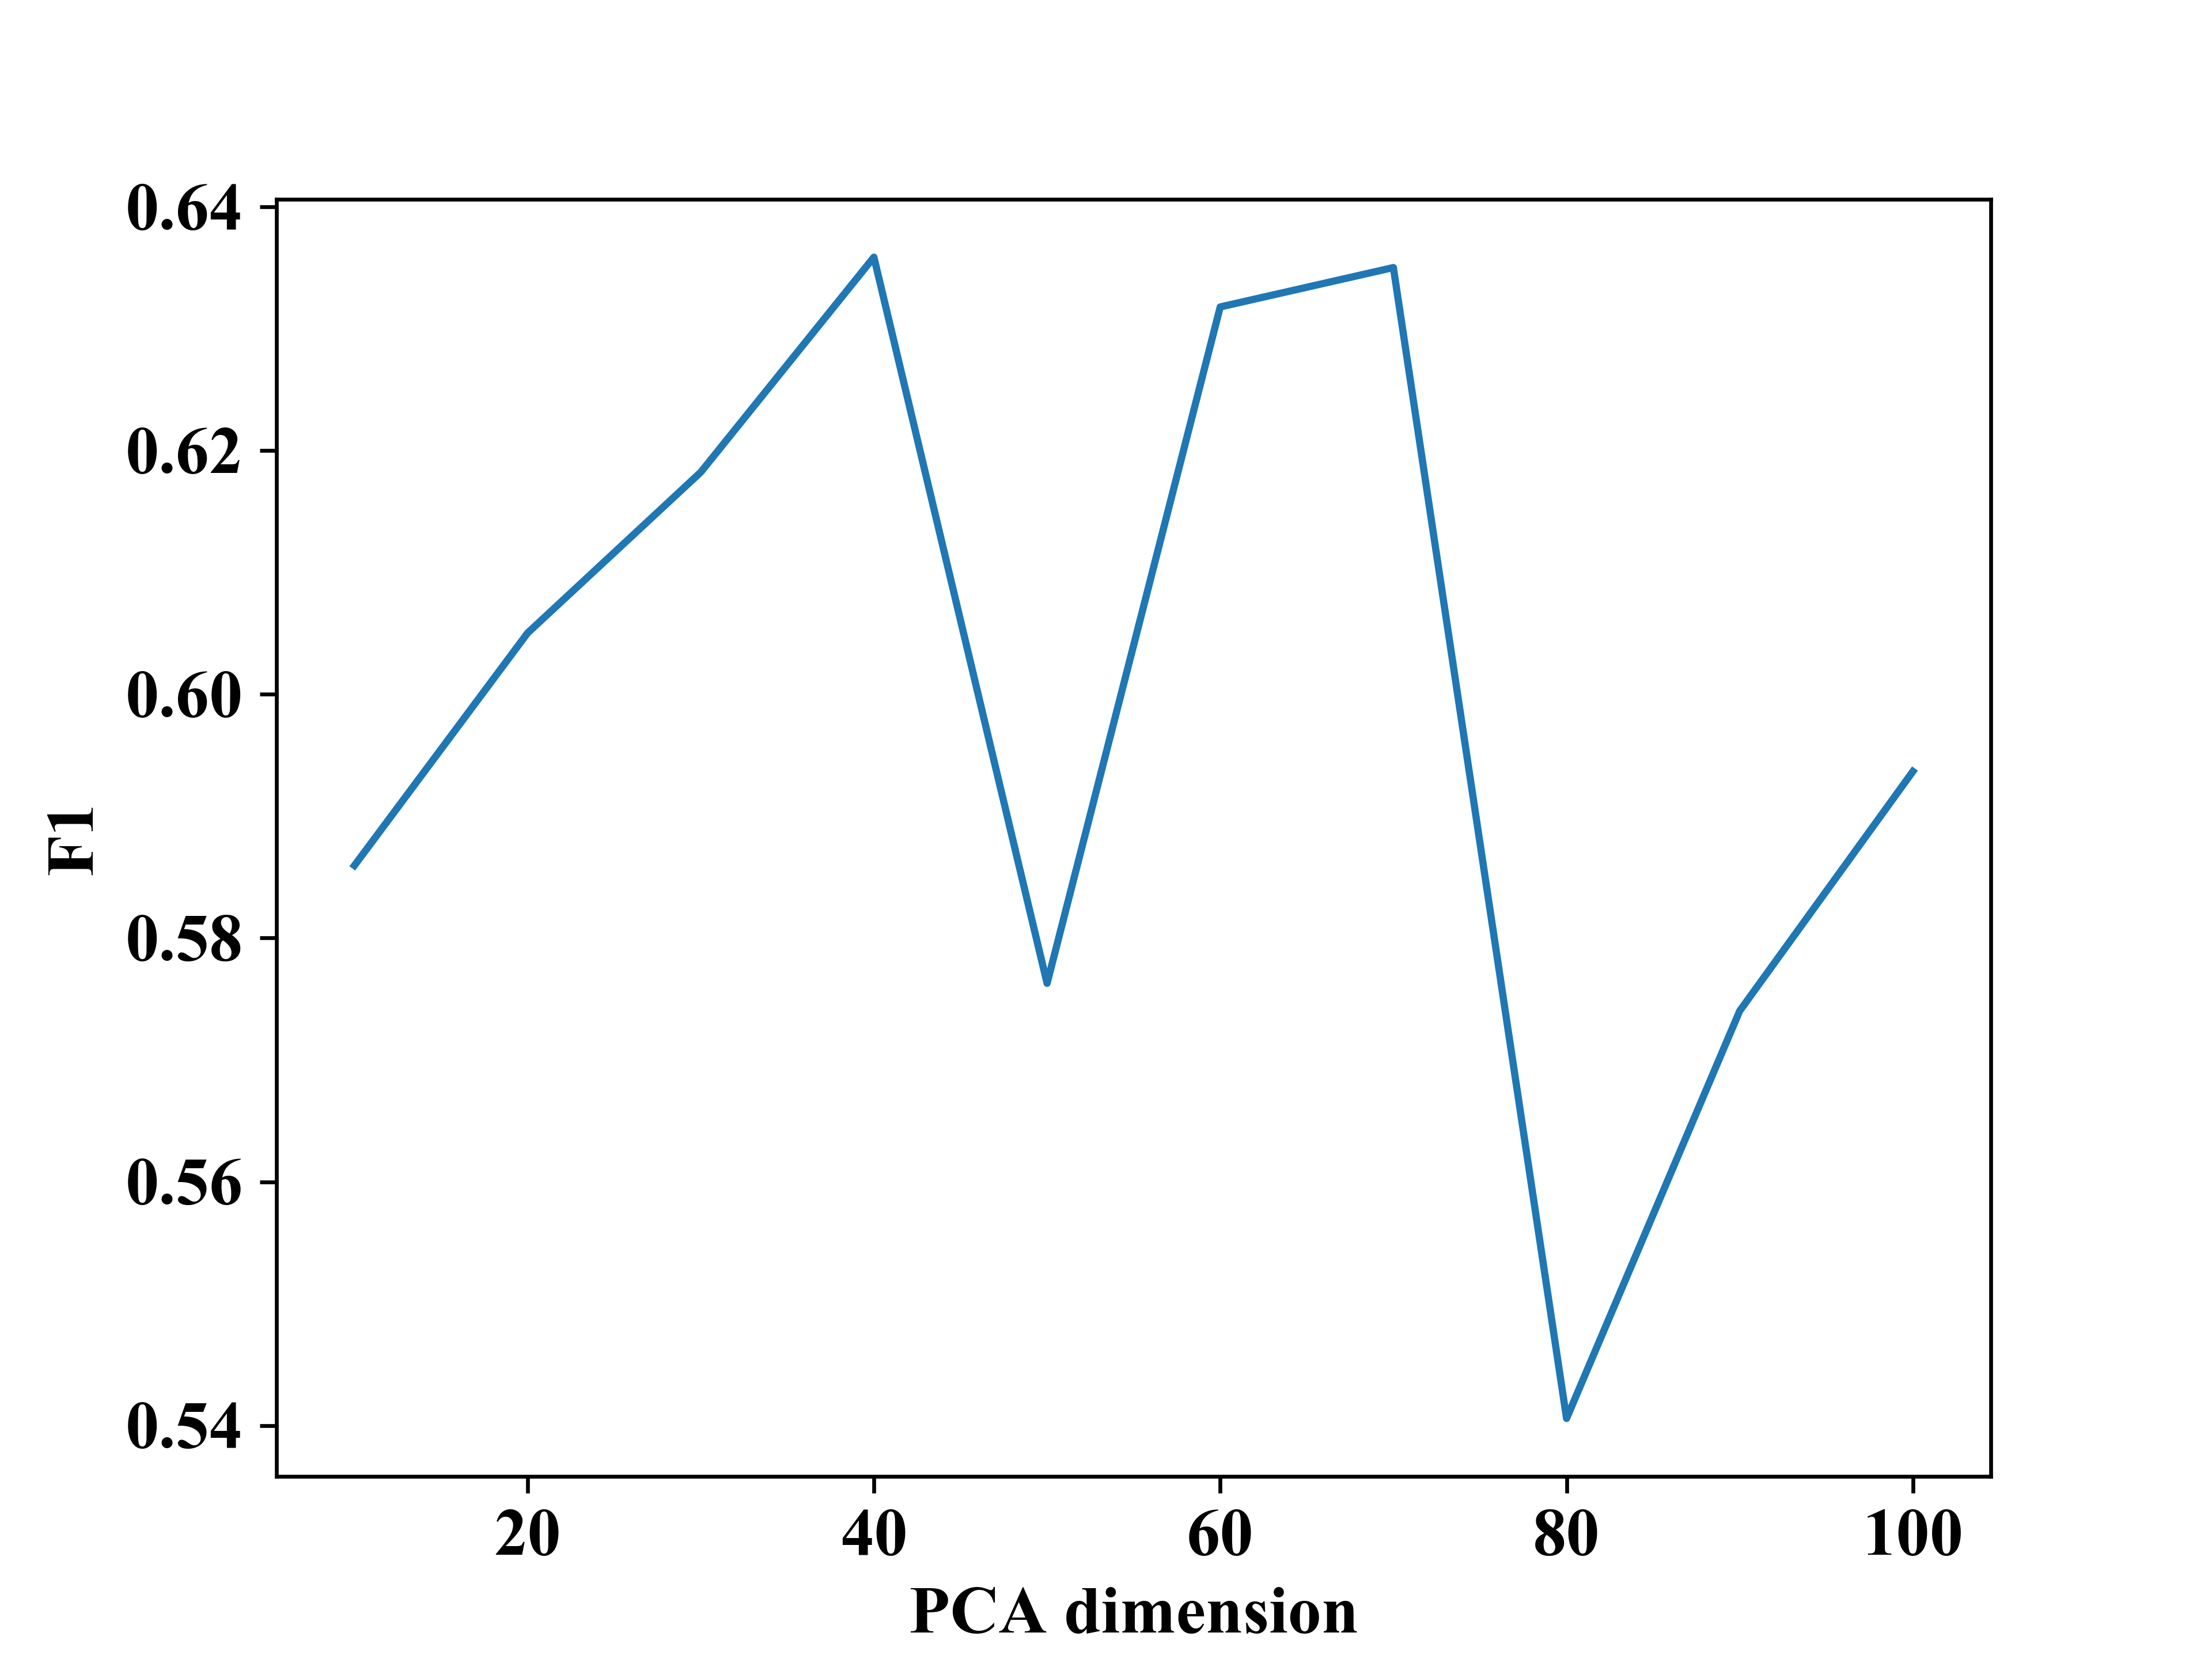
\includegraphics[width=0.5\textwidth]{./figures/cluster_f1.png}
%   \centering
%   \caption{f1随d的变化图}
%   \label{cluster_f1}
% \end{figure}

首先根据上述五个实验结果图,可以看出,当PCA降维的维度为40时,模型聚类的效果最好。但是仔细看会发现模型预测的$accuracy$,$F1$等值并不是很高,这与我们常见的其他机器学习模型进行分类的结果相差甚远,因此产生了疑问。我们现将聚类的结果的中心店进行可视化,如图~\ref{GMM_means}所示,可见直接聚类的效果并不一定较优,可能出现类别中心重复的现象。再经过仔细检查后发现,其实是预测方法存在一定的漏洞,虽然GMM模型将原始的数据集聚成10个簇,但是在预测标签时,可能会出现不同的簇它们出现最多的标签是同一个,此时会导致最后预测的标签只剩下不到10个类别,因此会丢失很多信息,导致了这样准确率不高的结果。

\subsubsection{单独聚类}

在这个任务中,可以设置不同个数的数字书写方式,即GMM的component的个数,而GMM的类中心初始化方式通常有Kmeans初始化以及随机初始化,对于GMM模型类与类之间的关系,存在独立和相关两种考量,分别对应对角线协方差矩阵以及非对角线对称矩阵。对这些变量进行评估,我们可以得到如图~\ref{fig:2-contrast} 的结果。

\begin{figure}[!h]
  \centering
  \subfigure[]{
    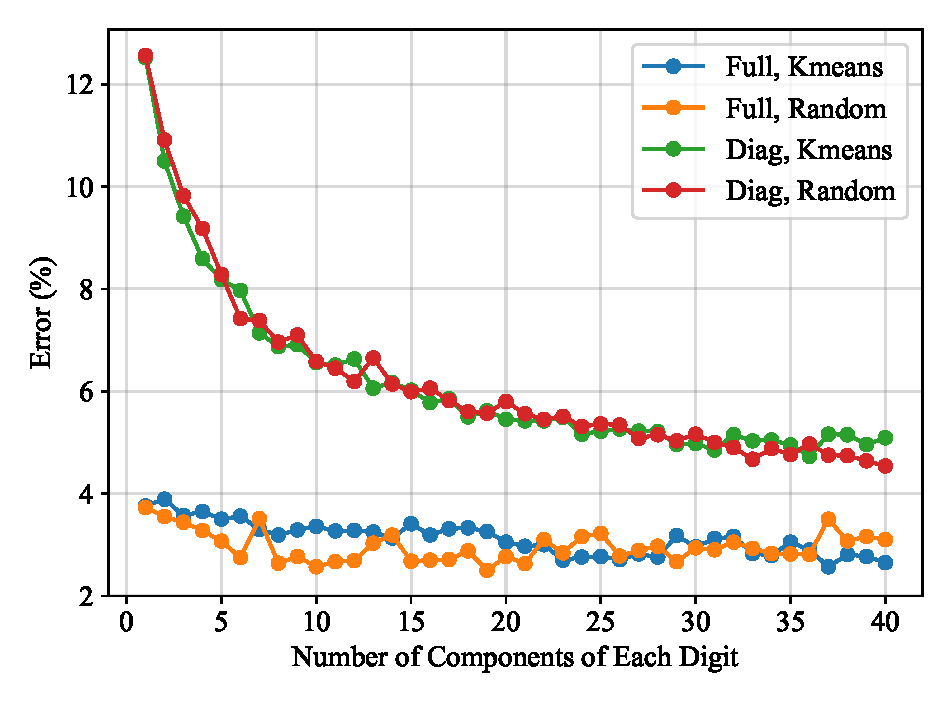
\includegraphics[width=0.45\textwidth]{figures/err.pdf}\label{fig:2-err}
  }\quad  
  \subfigure[]{
    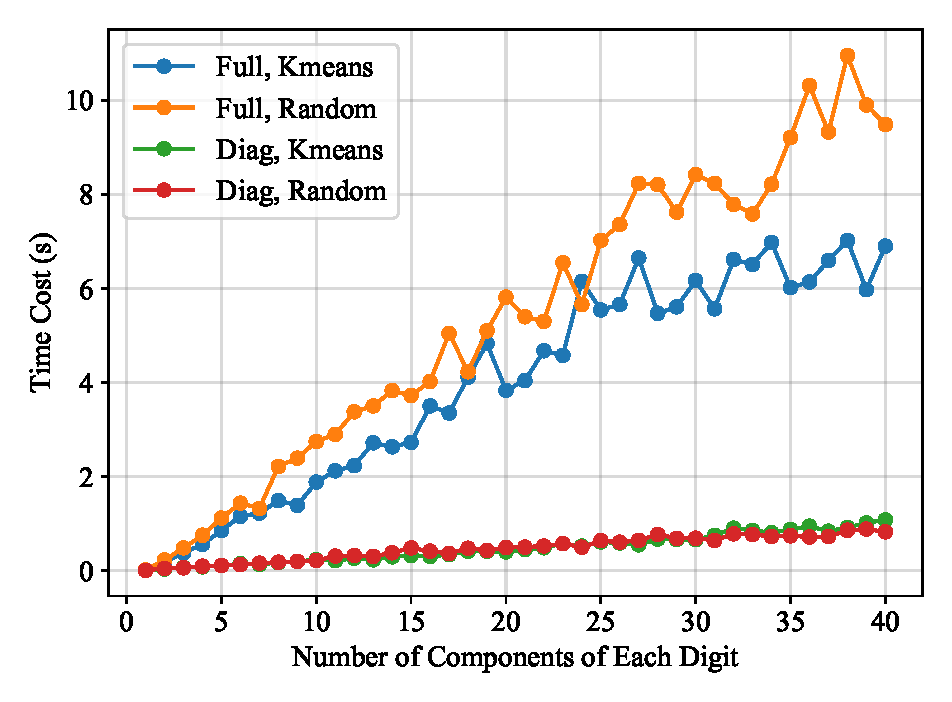
\includegraphics[width=0.45\textwidth]{figures/cost.pdf}\label{fig:2-cost}
  }
  \caption{不同的类中心初始化方式以及不同的协方差矩阵下,评估不同的分量个数对于分类误差和训练时间的影响。Full、Diag分别对应类与类之间独立和相关,Kmeans、Rand分别对应Kmeans初始化和随机初始化类中心。}\label{fig:2-contrast}
\end{figure}

\begin{figure}[!h]
  \centering
  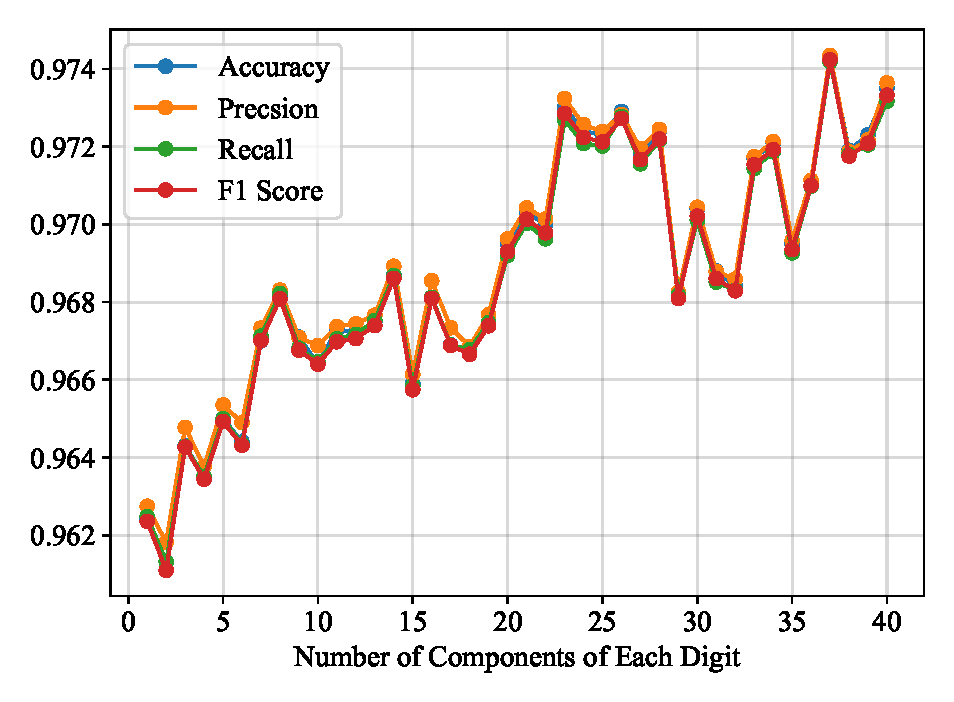
\includegraphics[width=0.5\textwidth]{figures/4metric.pdf}
  % \subfigure[]{
  %   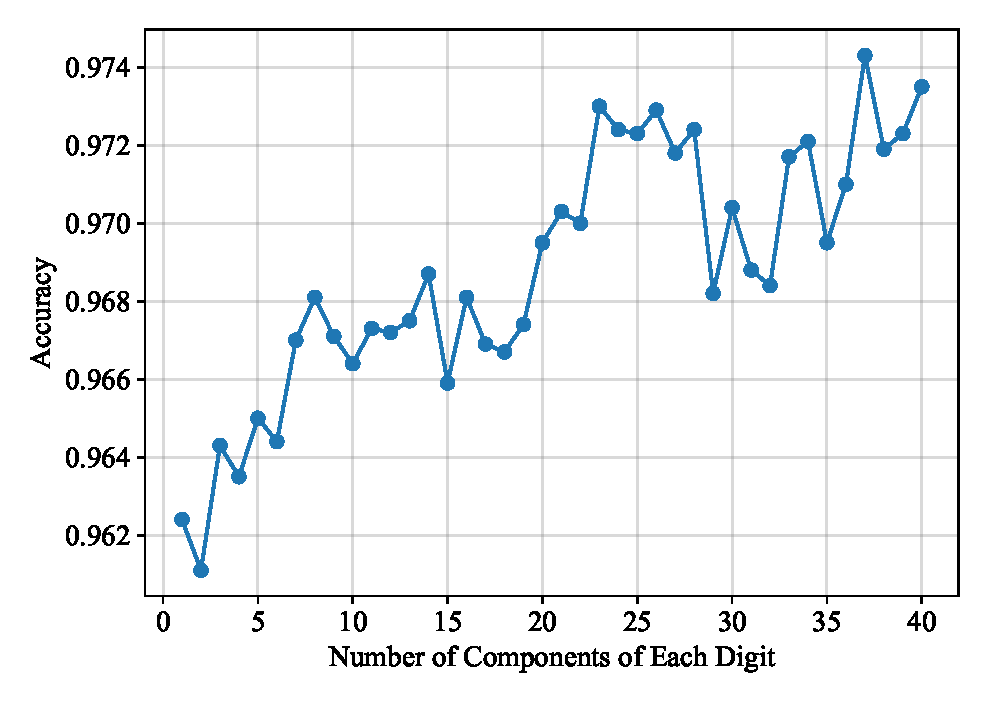
\includegraphics[width=0.22\textwidth]{figures/acc.pdf}\label{fig:2-acc}
  % }\quad
  % \subfigure[]{
  %   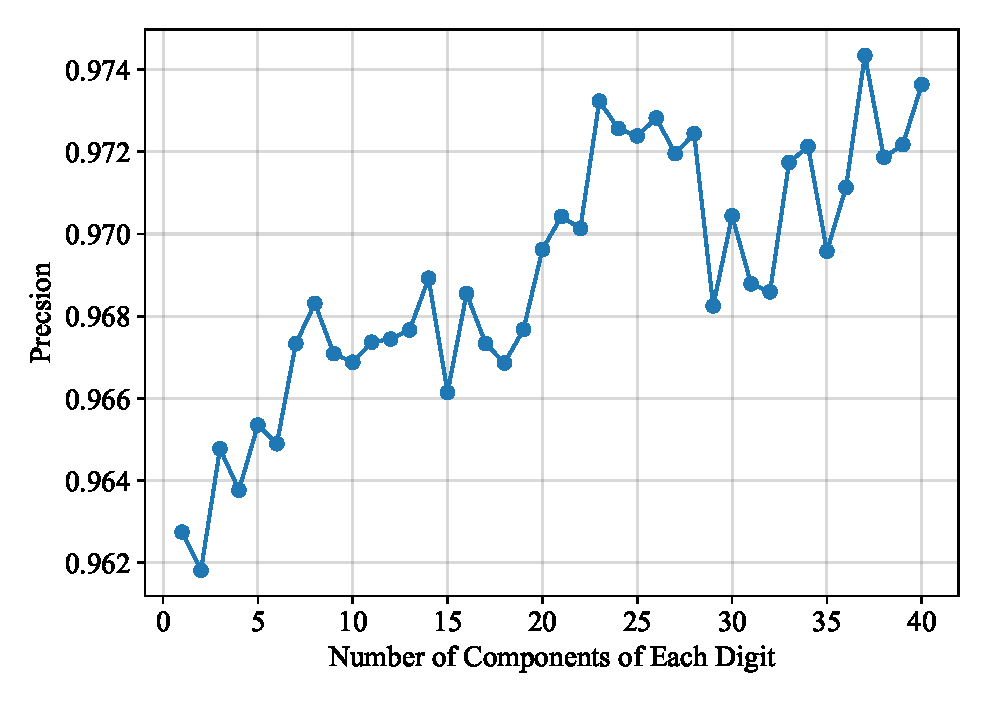
\includegraphics[width=0.22\textwidth]{figures/p.pdf}\label{fig:2-p}
  % }\quad
  % \subfigure[]{
  %   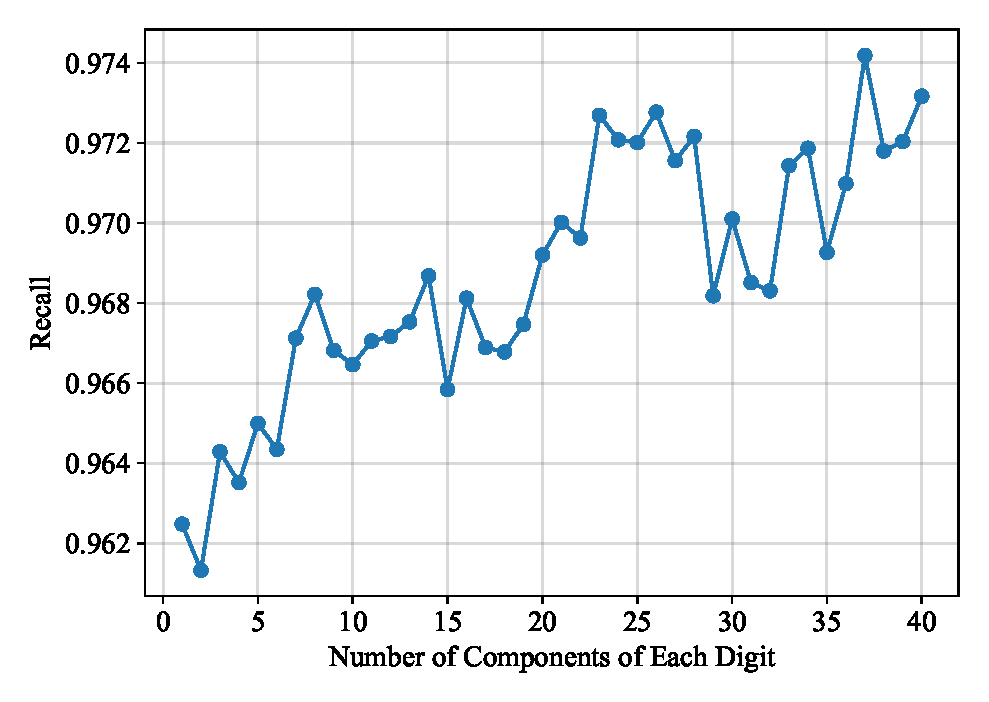
\includegraphics[width=0.22\textwidth]{figures/r.pdf}\label{fig:2-r}
  % }\quad  
  % \subfigure[]{
  %   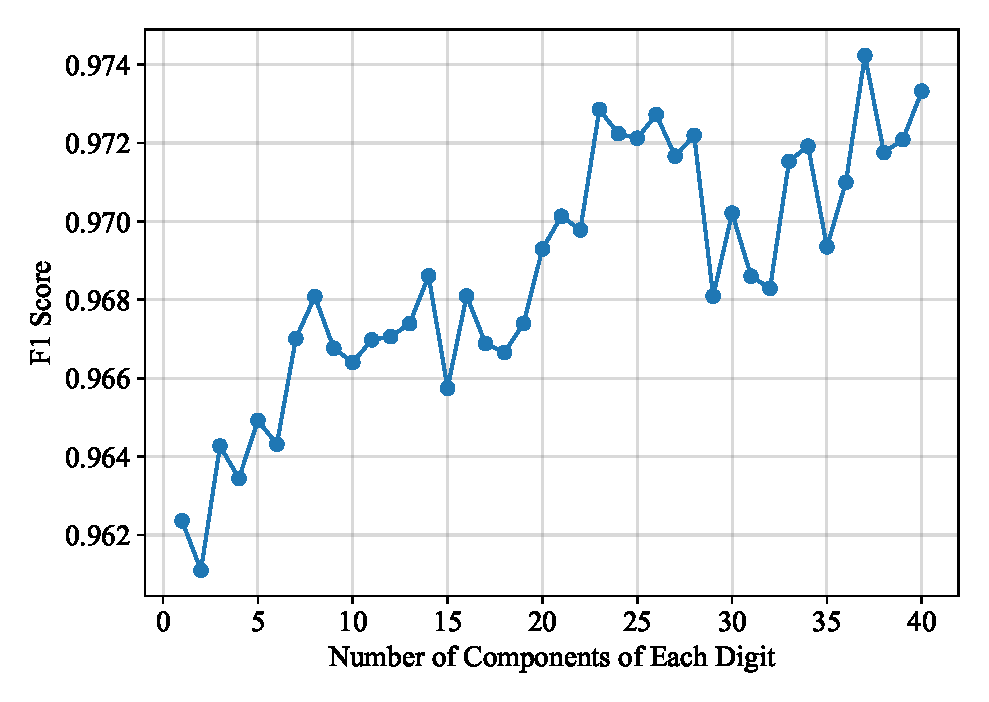
\includegraphics[width=0.22\textwidth]{figures/f1.pdf}\label{fig:2-f1}
  % }
  \caption{考虑类与类之间不独立,用Kmeans初始化类中心的前提下,四种评测指标随分量个数的变化。}\label{fig:2-4metrics}
\end{figure}

\begin{figure}[!h]
  \centering
  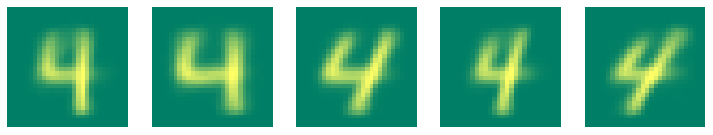
\includegraphics[width=0.8\textwidth]{./figures/diff4.pdf}
  \vspace{-.3cm}\caption{数字4的5种不同写法}\label{fig:diff4}
\end{figure}

从图~\ref{fig:2-err} 可以看到,若假设类与类之间相互独立,则其效果较差,因为不同类之间一般并非完全独立,都存在相互影响的关系,但是由于不考虑类之间的关系会使得计算变得很容易,因此时间消耗会相对应地减少(如图~\ref{fig:2-cost})。在考虑类与类之间不独立的情况下,我们还可以发现,随机初始化类中心会稍微比较耗时,同时其性能波动较大,但是整体趋于稳定,且在分量个数小于22的时候,其性能一般比Kmeans初始化要好。而Kmeans初始化的效果在随着分量个数增加而逐步降低,趋势性较强。

图~\ref{fig:2-4metrics} 展示了考虑类与类之间不独立,用Kmeans初始化类中心的前提下,四种评测指标随分量个数的变化,可以看到四种指标基本不相上下,说明我们的模型很可靠。最终,我们的单独聚类模型得到的类均值展示如图~\ref{fig:diff4} 所示,可以看到,每个数字都存在一些不同的写法,包括书写字体、书写角度以及书写清晰度,由此可见,对每一个数字类别单独聚类是非常有必要的。

% \begin{figure}[!h]
%   \centering
%   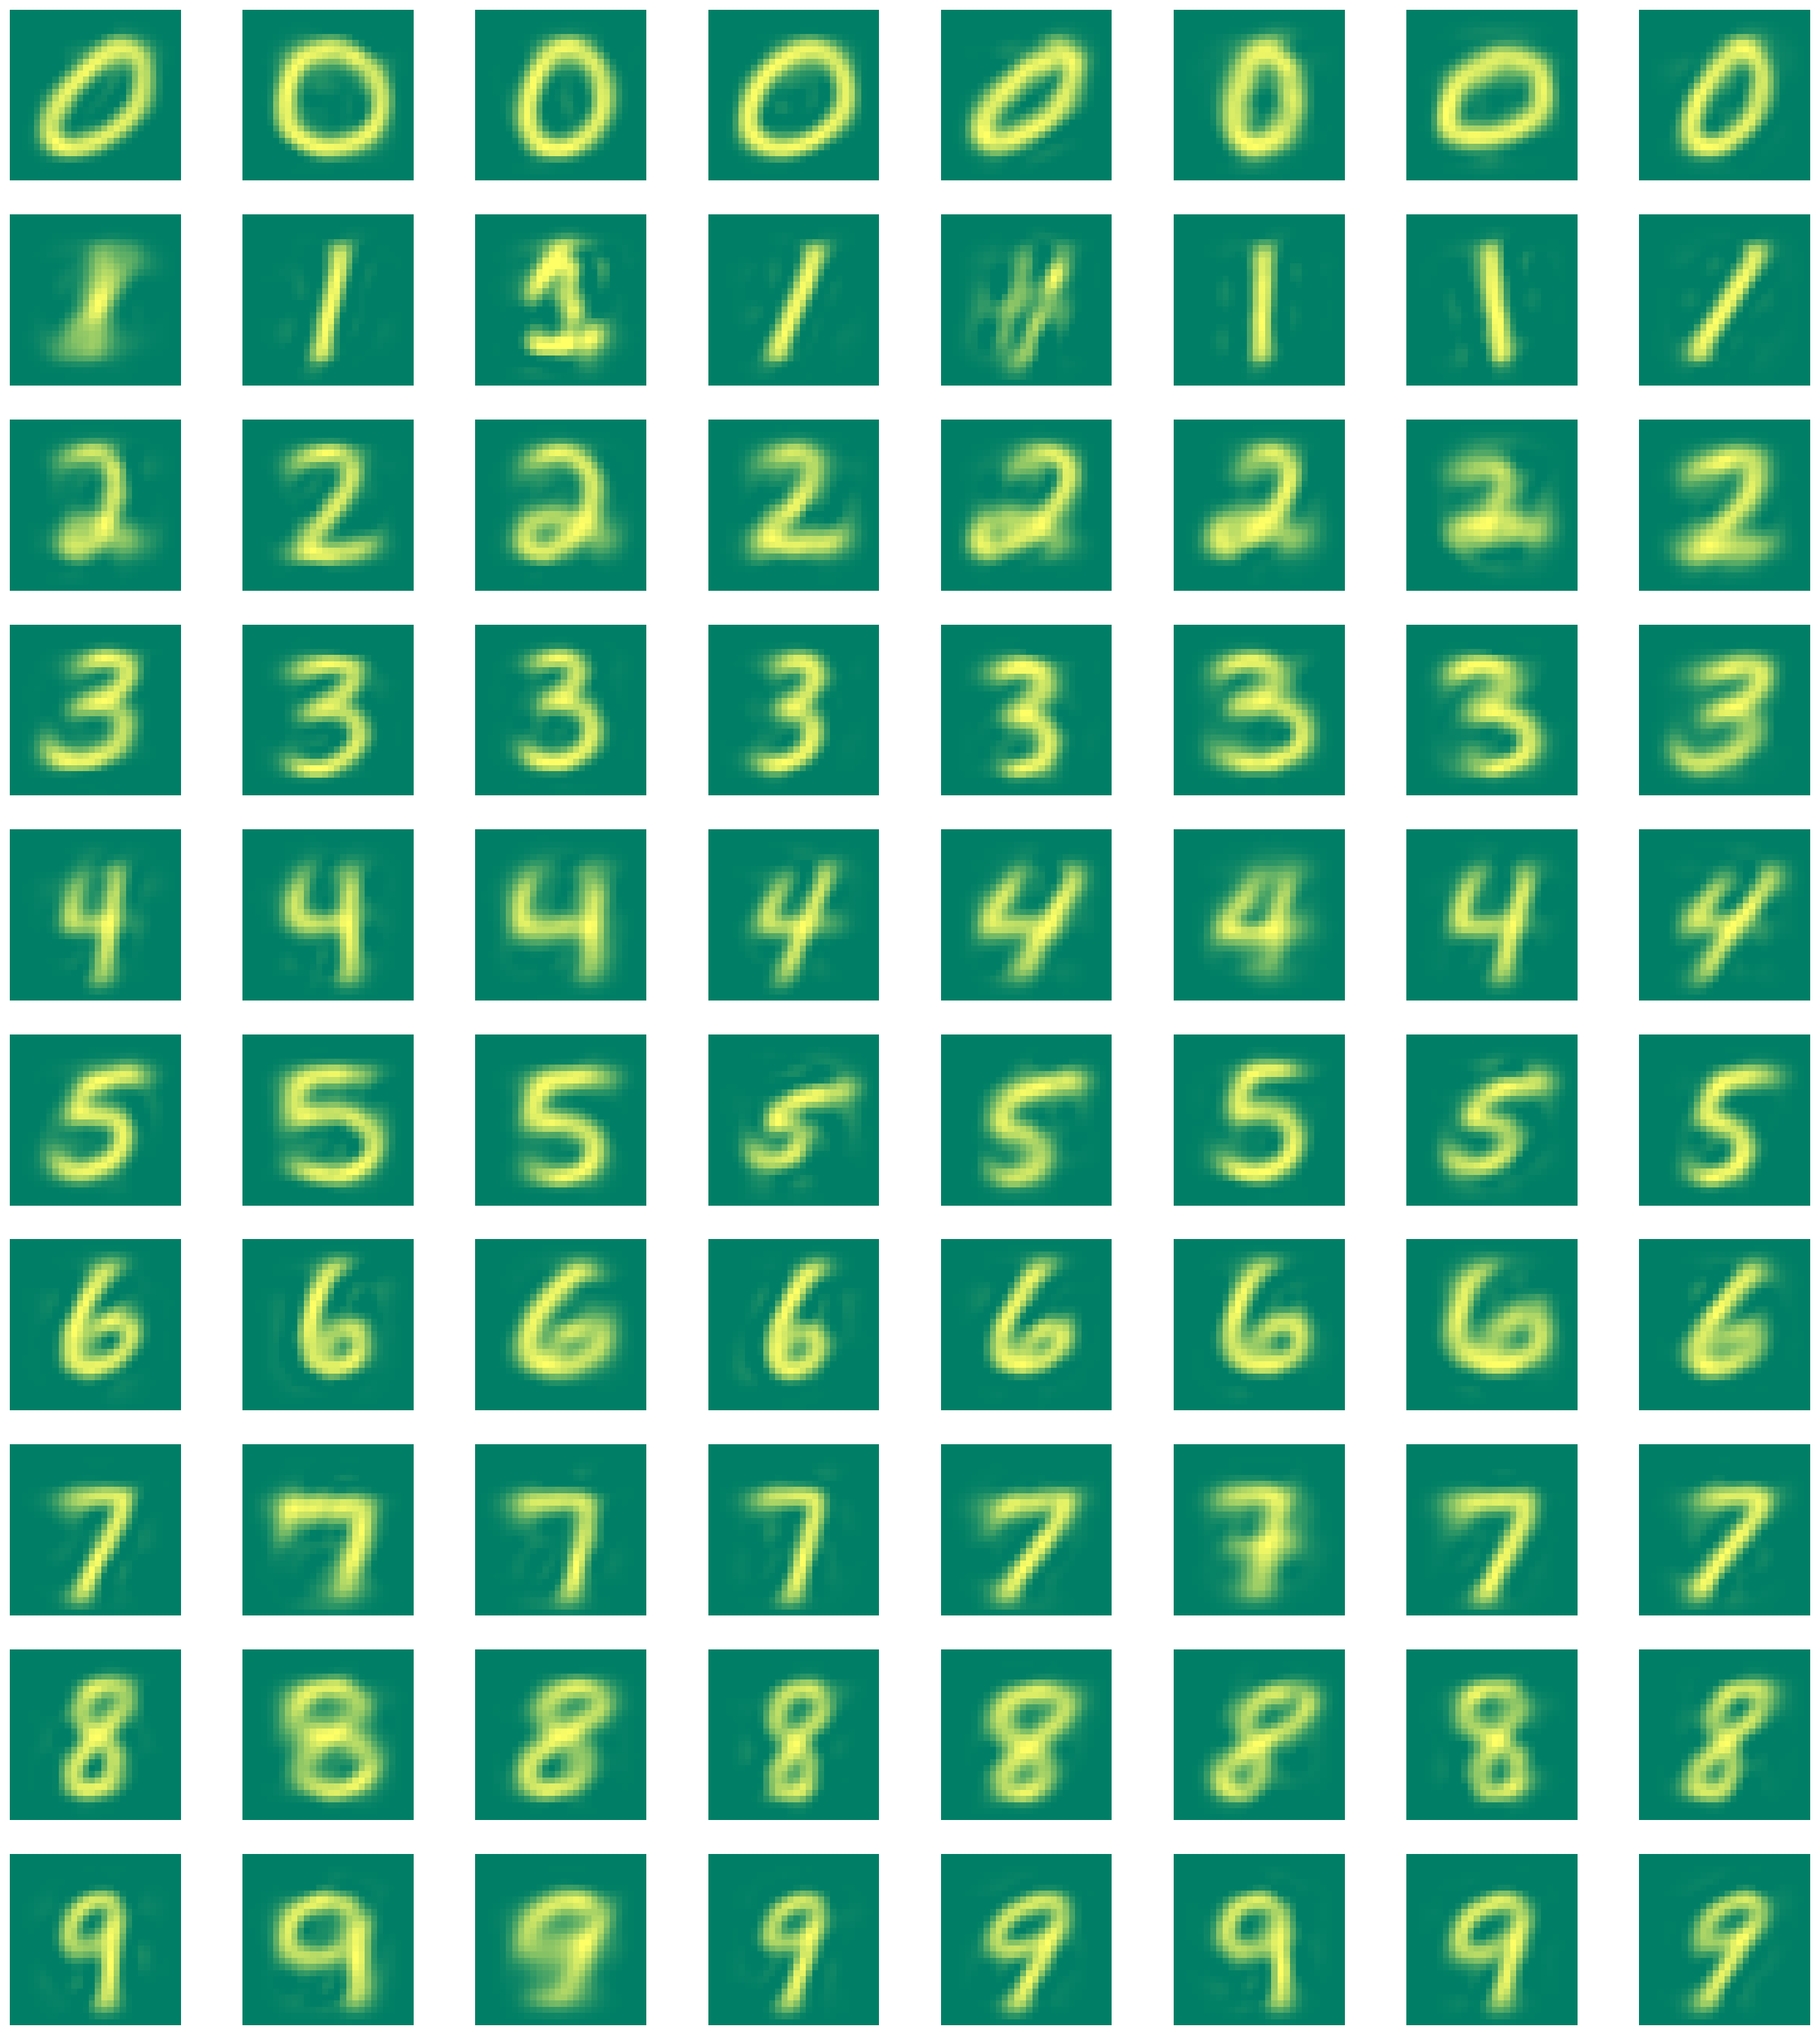
\includegraphics[width=0.9\textwidth]{figures/digits.pdf}
%   \vspace{-.3cm}\caption{单独聚类模型的各个类均值展示}\label{fig:2-class_means}
% \end{figure}

\subsubsection{生成手写数字}
生成的手写数字如图\ref{gen_digit}:
\begin{figure}[!h]
	\centering
	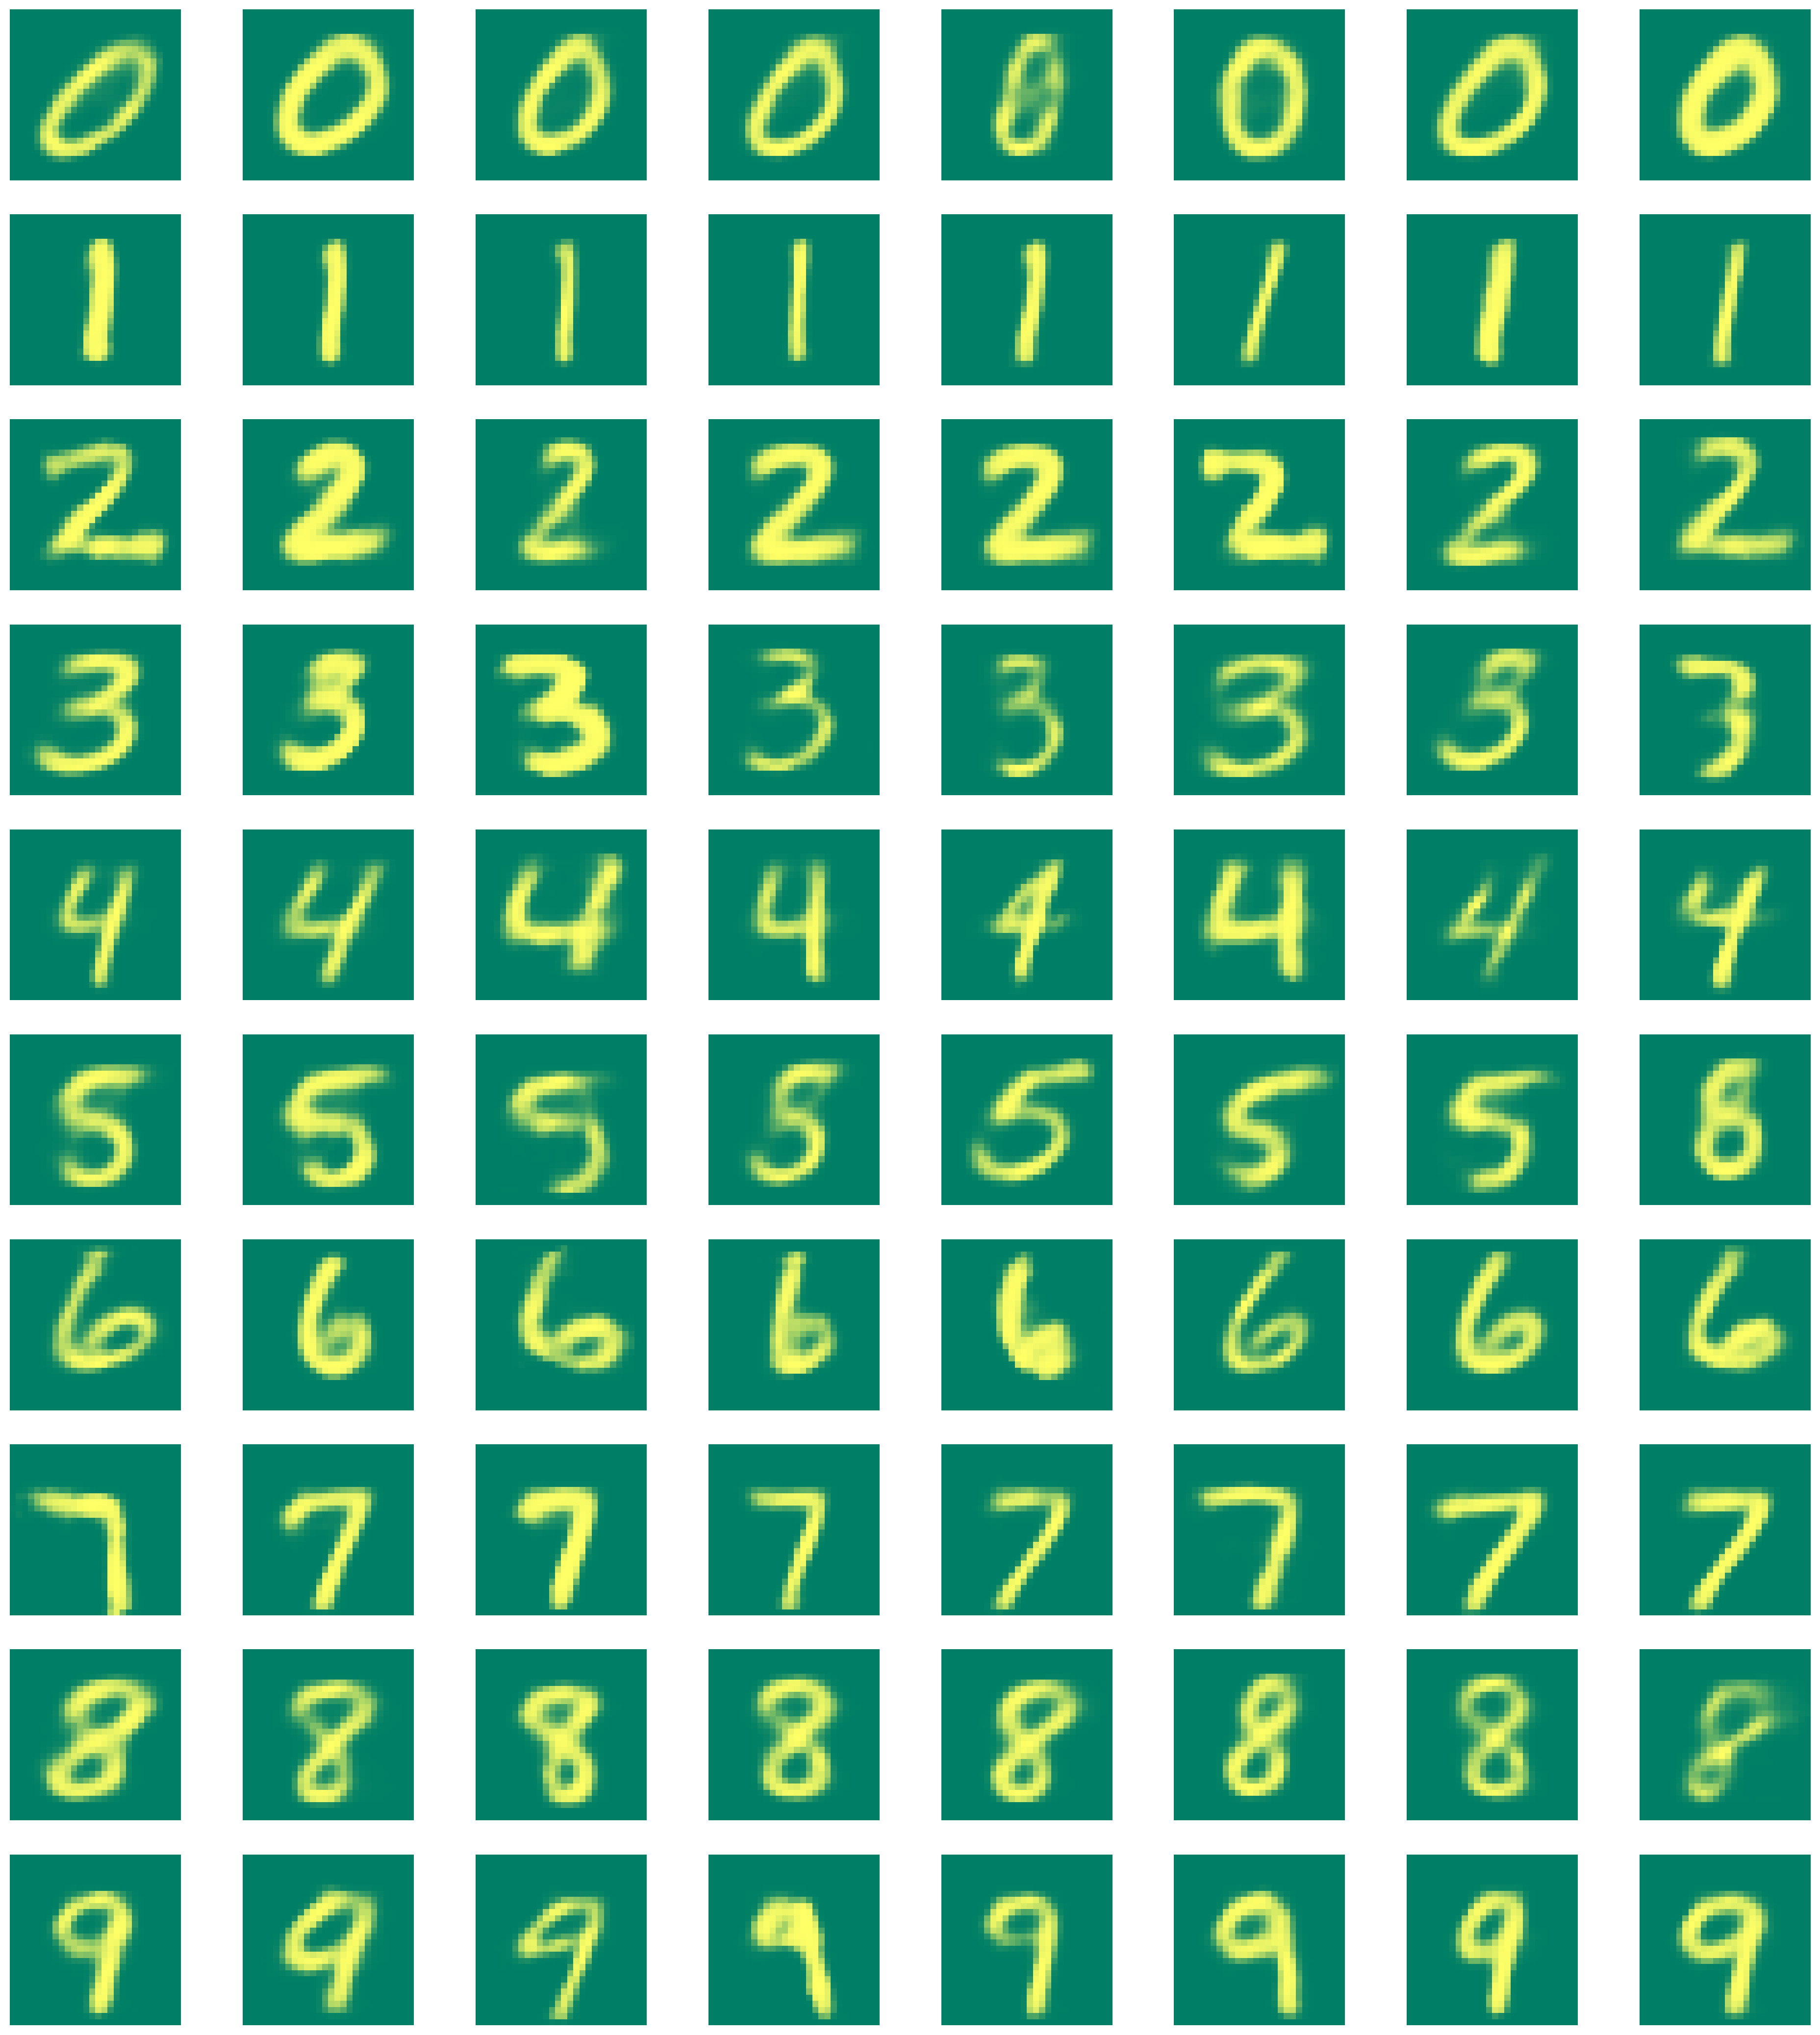
\includegraphics[width=0.8\textwidth]{./figures/gen0-9.png}
	\caption{生成手写数字0-9}
	\label{gen_digit}
\end{figure}

由于个别手写数字本身较为相像,以及前面提到的同一数字有着不同书写方式的原因,可能结果不是很准确。比如图中,部分“5”看上去更像数字“8”。但创造的新数字大体上还是符合0-9的书写方式的。

到这里,用GMM实现手写数字生成的任务就完成了。给定一个手写数字的样本,我们已经模拟了数据的分布,这样我们就可以从数据中生成全新的数字样本:这些是“手写数字”,不是直接来源于原始数据集,而是捕获了混合模型建模的输入数据的一般特征。

\section{展望}

\subsection{GMM的当前发展}

GMM在实际应用中十分广泛,比如语音识别、图像生成、以及各种聚类。

在语音识别方面,早于1995年,Douglas A. Reynolds和R.C.Rose就提出论文,基于GMM实现了独立于文本的语音识别。构成高斯混合的各个高斯分量用于对说话者的频谱从不同角度建模。他们在一个有49名讲话者的电话会议的语音上进行了测试,使用五秒的清晰语音即可获得96.8\%的识别准确度,在当时取得了极佳的效果。同年,Douglas A. Reynolds将GMM在更大的测试集上进行了测试。在TIMIT和NTIMIT数据库上(630位说话人)的闭集识别精度分别为99.5%和60.7%,在Switchboard数据集(113位说话人)上的识别准确率为82.8%。2000年,Douglas A. Reynolds和Thomas F.Quatieri以及Robert B.Dunn发表了论文。对已经在几个NIST语音识别评估(NIST Speaker Recognition Evaluations,SREs)中取得良好表现的语音识别模型的主要结构进行了描述,该模型由麻省理工学院林肯实验室开发,基于GMM。

在计算机视觉方面,2004年 Z. Zivkovic 提出了基于GMM的一种高效的自适应算法来进行背景提取,该模型可以不断更新参数,同时为每个像素选择适当数量的成分(component)。2005年Dar-Shyang Lee试图提高自适应高斯混合的收敛速度而不影响模型的稳定性。他将全局静态保留因子(global static retention factor)替换为在每帧处为每个高斯分布计算的自适应学习速率。结果显示该方法在合成视频数据和真实视频数据上都有更好的表现。该方法还可以与背景提取的统计框架结合,得到更好的图像分割性能。

在聚类方面,在《基于高斯混合模型的层次聚类算法》一文中, 作者提到计算高斯混合分布中每两个组成成分的重叠度,然后根据重叠的程度,即重叠率是否大于一个阈值,决定是否将两个分布合并。如果合并了,就重新更新均值和方差。再具体的生产应用中,GMM算法可用于图像聚类以及文本聚类等任务。

\subsection{实验展望}

由于聚类任务是GMM算法的一大重要应用,在此我们选取图像聚类为导向,进行GMM算法的实验验证。我们使用简单的MNIST数据集,验证GMM算法在的聚类、分类、生成任务中的有效性。未来我们计划利用GMM模型来解决一些实际问题,比如图像分割、文本聚类、图像聚类任务、以及一些视频序列运动目标检测的应用。

\section{大作业总结}

本学期已经接近尾声,这份大作业也贯穿了《数据科学基础》课程的始终。三个月以来,我们小组分工合作、齐心协力,一起查阅资料,分工完成任务,对难以理解之处进行小组讨论,在这个过程中我们都从中学习了很多。完成本次大作业需要对基础理论有充分的理解,进而在此基础上进行实际的应用,对于我们的理论和实际技能都是一次很好的提升机会。课程大作业参照毕业设计的方式,按照开题、中期、答辩设置三个节点,这样有利于我们在时间上对大作业有一个整体的把握,更好地协调小组的工作进度,让大作业有条不紊地完成。

由于疫情的原因,我们的上课方式改成了线上进行,虽然不能在课堂上进行面对面的交流,但整体感觉也是很扎实的。每一章的知识点都在PPT和学习指导中详细介绍,在每周二的课堂时间老师也会细细梳理一遍,然后我们在总结学习笔记的过程中再进行查漏补缺,基础知识掌握得很牢固。如今作为研究生的我们尚未返校,学习具有极大的自主性,自由支配的时间和空间变得更多,学习形式也更为灵活多样,在自学的过程中我们也应该注重知识结构的把握,有意识地锻炼自己的科学研究能力,不断提升理论水准,并将知识与能力结合。学习是一个长期积累的过程,在以后的工作、生活中都就应不断地学习,努力提高自我知识和综合素质。

本学期以来,我们都从《数据科学基础》课程中学习到了很多知识,对于这门课程我们还有一些小小的建议。由于线上的特殊授课方式,老师和同学之间的交流互动似乎过少了。如果在课堂上增加一些互动的环节,或许同学们能更加积极地参与其中,老师也能更准确地掌握学生的学习状况。另外,学习笔记中大部分都是定义、原理、公式推导等理论型的题目,且大多都能在PPT的对应章节找到答案,这样可能会导致学生在学习时只是机械地做一些“知识搬运”的工作。可以考虑在作业中也增加一些开放性较强、偏应用型的题目,鼓励学生多思考,灵活运用所学的理论知识。

感谢老师和助教同学一学期以来的辛苦付出,你们辛苦了!

\section{小组同学分工说明}

\begin{table}[H]
\centering
\begin{tabular}{|c|c|c|c|}
\hline
    & 实验       & 文档                                            & PPT                      \\
\hline
王阁元 & 整体聚类   & \makecell[c]{应用问题描述撰写,整体聚类实验\\相关部分撰写,实验展望撰写}                  & 整体聚类PPT制作                \\
\hline
罗薇  & 手写数字生成 & \makecell[c]{GMM模型理论撰写,数据集与评估指标\\部分撰写,手写数字生成实验相关\\部分撰写,大作业总结撰写} & 手写数字生成PPT制作              \\
\hline
寄家豪 & 单独聚类   & \makecell[c]{极大似然估计、隐变量、EM算法\\理论撰写,单独聚类实验相关部分撰写}              & \makecell[c]{PPT讲解,理论、问题描述、\\单独聚类的PPT制作} \\
\hline
\end{tabular}
\end{table}



\clearpage

\begin{thebibliography}{99}
	\bibitem{ref1}Wu M, Zhang Z. Handwritten digit classification using the mnist data set[J]. Course project CSE802: Pattern Classification \& Analysis, 2010.
	\bibitem{ref2}Gupta L, Sortrakul T. A Gaussian-mixture-based image segmentation algorithm[J]. Pattern Recognition, 1998, 31(3): 315-325.
	\bibitem{ref3}McLachlan G J, Krishnan T. The EM algorithm and extensions[M]. John Wiley \& Sons, 2007. 
	\bibitem{ref4}Dempster A P, Laird N M, Rubin D B. Maximum likelihood from incomplete data via the EM algorithm[J]. Journal of the Royal Statistical Society: Series B (Methodological), 1977, 39(1): 1-22. 
	\bibitem{ref5}Goodfellow I, Bengio Y, Courville A. Deep learning[M]. MIT press, 2016.
	\bibitem{ref6}周志华. 机器学习[M]. 北京:清华大学出版社, 2016.
	\bibitem{ref7}李航. 统计学习方法[M]. 北京:清华大学出版社, 2012.
	\bibitem{ref8}Bishop C M. Pattern recognition and machine learning[M]. springer, 2006.
	\bibitem{ref9}XIAO Z, WANG J. Image classification algorithm based on PCA and GMM[J]. Computer Engineering and Design, 2006, 27(11): 1951-1953.
	\bibitem{ref10}Bouman C A, Shapiro M, Cook G W, et al. Cluster: An unsupervised algorithm for modeling Gaussian mixtures[J]. 1997.
	\bibitem{ref11}陈雪峰. 图像高斯混合模型的判别学习方法[D].北京理工大学,2009.
	\bibitem{ref12}Xuan G, Zhang W, Chai P. EM algorithms of Gaussian mixture model and hidden Markov model[C]//Proceedings 2001 International Conference on Image Processing (Cat. No. 01CH37205). IEEE, 2001, 1: 145-148.
	\bibitem{ref13}Reynolds D A. Gaussian Mixture Models[J]. Encyclopedia of biometrics, 2009, 741.
\end{thebibliography}

\end{document}